%% LyX 2.0.5.1 created this file.  For more info, see http://www.lyx.org/.
%% Do not edit unless you really know what you are doing.
\documentclass[12pt,english]{report}
\usepackage{mathptmx}
\renewcommand{\familydefault}{\rmdefault}
\usepackage[T1]{fontenc}
\usepackage[latin9]{inputenc}
\usepackage[a4paper]{geometry}
\setcounter{secnumdepth}{2} % Changed from 3 to 2. 0-chapter 1-section 2-subsection 
\setcounter{tocdepth}{2} % Changed from 3 to 2. 0-chapter 1-section 2-subsection 
\setlength{\parskip}{\medskipamount}
\setlength{\parindent}{0pt}
\usepackage{verbatim}
\usepackage{pdfpages}
\usepackage{graphicx}
\usepackage{subfig} %% This package has to be here
\usepackage{setspace}
\usepackage{arabtex}
\usepackage[numbers]{natbib}
\usepackage{nomencl}

%Packages Added By George
\usepackage[linesnumbered]{algorithm2e}
\usepackage{color}
\usepackage{amsthm}
\usepackage{amsmath}
\usepackage{bbold}

% Theorem Styles
\newtheorem{theorem}{Theorem}[section]
\newtheorem{lemma}[theorem]{Lemma}
\newtheorem{proposition}[theorem]{Proposition}
\newtheorem{corollary}[theorem]{Corollary}
% Definition Styles
\theoremstyle{definition}
\newtheorem{definition}{Definition}[section]
\newtheorem{example}{Example}[section]
\theoremstyle{remark}
\newtheorem{remark}{Remark}

\usepackage{etoolbox}
\newtoggle{edit-mode}
\togglefalse{edit-mode}  
%\toggletrue{edit-mode}
\iftoggle{edit-mode}{
\geometry{verbose,tmargin=2cm,bmargin=2cm,lmargin=2cm,rmargin=6cm,headheight=1cm,headsep=1cm,footskip=1cm, marginparwidth=5cm}
}{
\geometry{verbose,tmargin=2cm,bmargin=2cm,lmargin=2cm,rmargin=2cm,headheight=1cm,headsep=1cm,footskip=1cm}
}

% the following is useful when we have the old nomencl.sty package
\providecommand{\printnomenclature}{\printglossary}
\providecommand{\makenomenclature}{\makeglossary}
\makenomenclature
\doublespacing

\makeatletter

%%%%%%%%%%%%%%%%%%%%%%%%%%%%%% User specified LaTeX commands.
\usepackage{tauthesis}
%\usepackage[font={small,bf}, labelfont={small,bf}, margin=1cm]{caption}
\usepackage{titlesec}
\newcommand{\hsp}{\hspace{20pt}}
\titleformat{\chapter}[hang]{\Huge\bfseries}{\thechapter\hsp}{0pt}{\Huge\bfseries}


\Title{\textbf{Ongoing Arabic On-line Handwriting Recognition}}
\Author{George Kour}
\Year{May 2014}
\Supervisor{Prof. Dana Ron}
\Supervisor{Dr. Raid Saabne}
\Department{School of Electrical Engineering}
\Degree{Master of Science}

\makeatother

\usepackage{babel}
\begin{document}

\prelimpages

\titlepage

\acknowledgments{
I would like to thank my instructor, Professor Dana Ron, for her assistance, inspiration and invaluable help in this research and her insightful comments on this thesis.

My sincere thanks also go to my second instructor, Dr. Raid Saabne, for introducing me to the field of handwriting recognition; for his endless efforts pushing me forward in time that it seems to be I am standing still; for believing in me and directing me through the hard times and giving me invaluable advices that I will take for life.

There is a famous statement in Arabic that was used to be written on the walls of schools which I would like to dedicate to you, dear instructors, and to all my teachers to express my deep appreciation.

\begin{center}
\RL{man `llmny .hrfaN, .sorto laho `bdaN Arb`yn `AmaN}\\
''For him, who has taught me even a single letter, I will be a servant for forty years'' 
\end{center}

Finally, I would like to give special thanks to my parents and brothers for their unconditional support and love during my whole life. 
They have always been there to support me and especially during this period. 
Words alone cannot express my deep emotions for them.
}

\cleardoublepage
\setcounter{page}{1} % Start preliminary pages numbering (roman numerals).
%%% LyX 2.0.5.1 created this file.  For more info, see http://www.lyx.org/.
%%% Do not edit unless you really know what you are doing.
%\documentclass[english]{report}
%\usepackage[T1]{fontenc}
%\usepackage[latin9]{inputenc}
%\setcounter{secnumdepth}{3}
%\setcounter{tocdepth}{3}
%\usepackage{setspace}
%\onehalfspacing
%\usepackage{babel}
%\begin{document}

\chapter*{Abstract}
 
Correct and efficient recognition of handwritten Arabic text is considered to be an essential problem due to the cursive and unconstrained nature of the Arabic script.
While real-time performance is necessary in applications involving on-line handwriting recognition, conventional approaches usually wait until the entire curve is traced out before starting the analysis, inevitably causing delays in the recognition process. 
This deferment restricts on-line recognition techniques to meet the highly responsiveness demands expected from such systems, and prevents implementing advanced features of input typing, such as automatic word completion and real-time automatic spelling.

This work proposes a real-time approach for segmenting and recognizing handwritten on-line Arabic script.
It demonstrate the feasibility of carrying out time consuming analysis and classification tasks during the course of writing. 
The presented real-time recognition-based segmentation method is facilitated using a fast letters classifier. 
It employs linear-time embedding technique of the feature space into the wavelet coefficient normed space, facilitating the usage of state-of-the-art, fast and accurate similarity measure and search techniques.
We show that the resulted segmentation and letters classification information can be used to significantly reduce the potential dictionary size and accelerate a later holistic recognition process.

The system has been designed and tested using the ADAB Database, and promising results were obtained.
 
%\end{document}


\tableofcontents{}

\listoffigures

\listoftables

\printnomenclature{}

\textpages

%% LyX 2.0.5.1 created this file.  For more info, see http://www.lyx.org/.
%% Do not edit unless you really know what you are doing.
%\documentclass[12pt,english]{report}
%\usepackage{mathptmx}
%\renewcommand{\familydefault}{\rmdefault}
%\usepackage[T1]{fontenc}
%\usepackage[latin9]{inputenc}
%\usepackage[a4paper]{geometry}
%\setcounter{secnumdepth}{2} % Changed from 3 to 2. 0-chapter 1-section 2-subsection 
%\setcounter{tocdepth}{2} % Changed from 3 to 2. 0-chapter 1-section 2-subsection 
%\setlength{\parskip}{\medskipamount}
%\setlength{\parindent}{0pt}
%\usepackage{verbatim}
%\usepackage{pdfpages}
%\usepackage{graphicx}
%\usepackage{subfig} %% This package has to be here
%\usepackage{setspace}
%\usepackage{arabtex}
%\usepackage[numbers]{natbib}
%\usepackage{nomencl}
%\usepackage{amsthm}
%\usepackage{amsmath}
%\usepackage{amsfonts}
%\usepackage{paralist}
%\usepackage{etoolbox}
%\newtoggle{edit-mode}
%\toggletrue{edit-mode}  
%%%\toggletrue{edit-mode}
%\iftoggle{edit-mode}{
%\geometry{verbose,tmargin=2cm,bmargin=2cm,lmargin=2cm,rmargin=6cm,headheight=1cm,headsep=1cm,footskip=1cm, marginparwidth=5cm}
%}{
%\geometry{verbose,tmargin=2cm,bmargin=2cm,lmargin=2cm,rmargin=2cm,headheight=1cm,headsep=1cm,footskip=1cm}
%}
%
%
%\begin{document}

%%%%%%%%%%% nomenclature %%%%%%%%%%
\nomenclature{HWR}{Handwriting Recognition}
\nomenclature{OCR}{Optical Character Recognition}
\nomenclature{WP}{Word Part}
\nomenclature{ANN}{Artificial Neural Network}
\nomenclature{SVM}{Support Vector Machine}
\nomenclature{$k$-NN}{$k$ Nearest Neighbours}
\nomenclature{SP}{Segmentation Point}
\nomenclature{POI}{Point Of Interest} 
%%%%%%%%%%%%%%%%%%%%%%%%%%%%%%%%%%%%

\chapter{Introduction}

\section{Background and Previous Work}

\subsection{Handwriting Recognition}
\iftoggle{edit-mode}{\hspace{0pt}\marginpar{HWR Motivation 1 - handwriting importance and survival}}{}
Writing has made much of the culture and civilization possible.
It was developed as a mean to expand human memory and to facilitate communication. 
Despite the long standing prediction that digital computers will challenge its future, handwriting remains a commonly used mean for communication and recording of information in the daily life; the pen and paper are still the natural medium for many important tasks such as notes taking in class. 
Therefore, a growing interest in the \emph{handwriting recognition} (HWR) field has emerged in recent years, and has now been a topic of research for over four decades.


\iftoggle{edit-mode}{\hspace{0pt}\marginpar{HWR Motivation 2 - ease of digital representation and Keyboard-less devices}}{}
Converting handwritten script into its digital analogous is highly motivated by the ease and convenience of the digital representation.
Not only this is useful for making digital copies of handwritten documents, but also in many automated processing tasks such as searching, indexing, automatic mail sorting, editing, sharing and more \cite{noaparast2009persian}.
Another motivation for recognizing handwritten scripts is the rapid transition from personal computers and laptops to the usage of keyboard-less smart-phone and table devices that are too small to have convenient keyboard, and thus, requiring pen or finger gestures to enter data \cite{connell2000online}. 

\iftoggle{edit-mode}{\hspace{0pt}\marginpar{HWR as OCR}}{} 
HWR was defined as "the task of transforming a language represented in its spatial form of graphical marks into its symbolic representation" by Plamondon and Srihari \cite{plamondon2000online}.
HWR is a special case of \emph{optical character recognition} (OCR), an important field in pattern recognition that is defined as the science of electronically converting a scanned, photographed, or sensed of both typewritten or printed texts, into machine-encoded text. OCR has been steadily evolving during its history and has always been a favorite testing ground for new ideas in pattern recognition, giving rise to an exciting set of research topics and producing many powerful practical applications.
However, since many experiments of new ideas in pattern recognition were conducted on isolated characters, the results are not always immediately reflected in OCR applications \cite{burrow2004arabic}  .
OCR is considered one of the best applications of machine vision and one of the most successful research branches in pattern recognition theory. 
Although considered a well developed technological field, OCR remains an area of active scientific research and creative engineering \cite{borovikov2004survey}.
Besides recognition, handwriting is associated with other types of analysis, such as signature verification, writer identification, etc.

\iftoggle{edit-mode}{\hspace{0pt}\marginpar{Levels of difficulties in HWR}}{}
There are different types of problems with varying complexity within HWR, depending on how the data is presented to the recognition system, at what level the data can be unambiguously broke into pieces (e.g. individual characters or words), and the transcription complexity of the language used \cite{bahlmann2005advanced}. 
In one extreme there is the case of isolated characters written inside graphical boxes in which the segmentation problem is already solved. The opposite extreme is the case of cursive unrestricted handwriting in which words, or portion of a word, is written with a single stroke, i.e, ligatures connect adjacent letters. HWR systems have a strong history in making use of this graduation in difficulty \cite{bahlmann2005advanced}. 

\iftoggle{edit-mode}{\hspace{0pt}\marginpar{State of the Art HWR}}{}
\emph{TODO: take that from the book.}

\iftoggle{edit-mode}{\hspace{0pt}\marginpar{Arabic HWR challenge}}{}
A script is a set of icons that have certain basic shapes. 
These are known as characters or letters.
Each script has its own rules regarding how letters are combined to form shapes that represent higher level linguistic units \cite{plamondon2000online}.
Unlike the Latin script, in which non-cursive handwriting, i.e., using isolated characters, is possible and common, Arabic is cursively written in both handwritten and printed text.
Its unconstrained nature, which produces a huge variety in the handwriting of different people, makes the recognition of Arabic script extremely difficult.
Figure \ref{fig:ha_different} shows several handwritten samples the letter \RL{.h} /.h/, in its isolated form, written by several writers.
Text segmentation, that is, the process of dividing a cursive writing into sub-units (typically characters) turns out to be a challenging task.

\begin{figure}
\centering
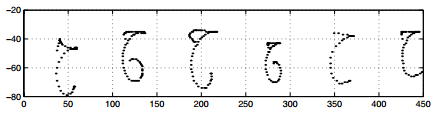
\includegraphics{./figures/ha_different}       
\caption{Different writing styles of the isolated form of the letter \RL{.h}.}
\label{fig:ha_different}
\end{figure}


%%%%%%%%%%%%%%%%%%%%%%%%%%%%%%%%%%%%%%%%%%%%%%
\subsection{Off-line versus On-line Handwriting Recognition}

\iftoggle{edit-mode}{\hspace{0pt}\marginpar{Introduction}}{}
The field of HWR can be classified in several ways. However, the most common categorization is the one that distinguishes between \emph{off-line} (also called static) and \emph{on-line} (also called dynamic).
Off-line HWR focuses on documents that have been written on paper at some previous point of time. A digital image of the document is fed to the computer, and the system attempts to convert the spatial representation of the letters into digital symbols \cite{al2011online}. 
In contrast, on-line HWR is performed on a digital representation of the text written on a special digitizer, tablet or smart-phone device, where sensors pick up the pen-tip movements and the two-dimensional coordinates of successive points of the writing as a function of time are stored.
Figure \ref{fig:offline_vs_online} shows typical input signals that can be analyzed in both cases.

\begin{figure}
	\centering
        \subfloat[]{
            \label{fig:offline}
            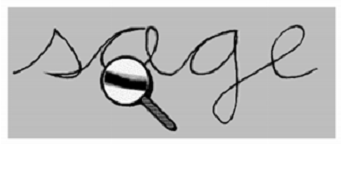
\includegraphics[width=0.5\textwidth]{./figures/offline}
        }
        \subfloat[]{
           \label{fig:online}
           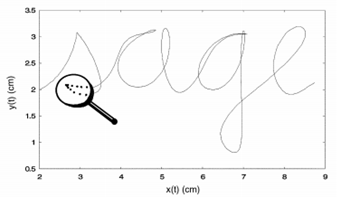
\includegraphics[width=0.5\textwidth]{./figures/online}
        }        
    \caption{An on-line vs. an off-line representation of a word \cite{plamondon2000online}.}
   \label{fig:offline_vs_online}
\end{figure}

\iftoggle{edit-mode}{\hspace{0pt}\marginpar{Literature}}{}
The research on on-line handwriting recognition started in the 1960's and has been receiving a great interest from the 1980's \cite{tagougui2013online}.
One of the earliest studies on On-line Arabic script recognition was carried out by El-Wakil and Shoukry in 1989 \cite{el1989line}.

\iftoggle{edit-mode}{\hspace{0pt}\marginpar{Similarities and advantages of on-line and off-line}}{}
Off-line HWR techniques can be applied to on-line data by constructing a static image of the on-line script. 
However, it has been shown that the information of the pen dynamics, such as the strokes breaking (i.e., "pen-down" and "pen-up" events) and the order of writing, can be used to obtain a better recognition accuracies than the static data alone. 
In the other direction, the success of on-line systems makes it attractive to consider developing off-line systems that first estimate the trajectory of the writing from the off-line data and then use on-line HWR techniques. 
Nevertheless, reconstructing the temporal data is problematic, and thus, has led to few such systems so far \cite{plamondon2000online}.

\iftoggle{edit-mode}{\hspace{0pt}\marginpar{off-line objectives}}{}
In general, off-line HWR systems are less accurate than on-line systems, but, they are now good enough that they have a significant economic impact on specialized domains such as interpreting handwritten postal addresses on envelopes and reading courtesy amounts on bank checks \cite{melin2007analysis}.

\iftoggle{edit-mode}{\hspace{0pt}\marginpar{A general flow for HWR}}{}
Despite the large variation among the different methods for HWR, there are several fundamental stages that are common between most of the systems.
The data acquisition step is the first stage in HWR. 
In the on-line case, the stylus motion is sampled at equal time intervals.
The samples go through a preprocessing stage that includes filtering of noises, re-sampling the stroke information to obtain equidistant stroke, and normalized to a standard size. 
Additional preprocessing may include slant and slope corrections. 
Then, depending on the nature of the system, the script may undergo segmentation into basic units that could be words, parts of words, single characters or graphemes.
Typically, a feature extraction technique is then applied to extract significant and distinguishing attributes of the input data.
Using a classification algorithm the basic units are labeled. 
In many cases, a post-processing stage is applied in which the language model is used to search for the most likely string in the lexicon.

\iftoggle{edit-mode}{\hspace{0pt}\marginpar{off-line HWR additional steps}}{}
Approaches for on-line and off-line handwriting recognition, while having much in common, are different, due to the disparity in the input data representation. 
Their different nature imposes different challenges and thus variable levels of efforts are required to be spent on the various stages.
The off-line HWR systems usually consist of additional steps of layout analysis and text lines extraction, which are activated at the beginning of the preprocessing stage. 
Each text line is then divided into words or WPs. 
The segmentation, in such system, is made into images that contain basic units. 
The whole process is straightforward for well printed or well written documents; however, in the case of historical or badly printed document much effort is invested in a preprocessing stage that include smoothing, writing flow reconstruction, purification, and more \cite{saba2010survey}. 

%%%%%%%%%%%%%%%%%%%%%%%%%%%%%%%%%%%%%%%%%%%%%%

\subsection{The Holistic versus the Analytic Approach}

\iftoggle{edit-mode}{\hspace{0pt}\marginpar{Importance of the dictionary size}}{}
The vocabulary, from which the words in the test set are taken, has a major impact on how difficult the HWR task is.

\iftoggle{edit-mode}{\hspace{0pt}\marginpar{Closed and open vocabulary definitions}}{}
Closed-vocabulary HWR systems are capable of recognizing words from a predetermined limited size dictionary. 
The restricted vocabulary set is usually called a lexicon.
There are no well-established criteria for the categorization of lexicon size. 
However, the following terms are usually used:
\begin{compactitem}
\item small lexicon - tens of words.
\item medium lexicon - hundreds of words.
\item large lexicon - thousands of words.
\item very large lexicon - tens of thousands of words.
\end{compactitem}
Open-vocabulary tasks refer to the recognition of any word without the constraint of being in a dictionary.

\iftoggle{edit-mode}{\hspace{0pt}\marginpar{Recognition difficulty}}{}
The lexicon is a key-point post-processing stage in many systems, because the linguistic knowledge helps to filter out many possible options that are not included in the lexicon, and consequently raises the recognition rate.
The adhesion to a limited dictionary, may also limit the computational complexity. 
Although most research efforts have been devoted to closed vocabulary systems, open vocabulary systems have also been proposed.
Yet, their accuracy is still far below those relying on a small vocabulary \cite{koerich2003large, shu1996line}.

\iftoggle{edit-mode}{\hspace{0pt}\marginpar{problems imposed by the open vocabulary}}{}
While there exists a wide variety of approaches to cursive script recognition, research in this field has established two main approaches, one is the analytic approach \cite{abdulla2008off, sari2002off, dinges2011offine, elanwar2012unconstrained}, and the other is the holistic approach \cite{biadsy2011segmentation}. 


The analytic approach involves segmentation of the input curve into basic units and the classification of each individual unit.
The advantage of this approach is that it requires to maintain only a small set of trained models - one for each letter shape - to handle large vocabulary. 
However, the absence of consistent baselines, large variations in writing styles, and seamless connection between letters (connection is done with almost no ligatures) makes segmentation into individual letters very challenging \cite{saabni2009hierarchical}.

\iftoggle{edit-mode}{\hspace{0pt}\marginpar{The holistic approach}}{}
The holistic approach considers the global properties of the written text and recognizes the input word shape as a whole. 
Most popular methods among this group are based on analysis of the number and order of ascenders, descenders, loops and vertical strokes; they often rely on heavy dictionary searching that is costly and prone to be mislead by spelling errors \cite{brodowska2011oversegmentation}.
While it avoids the error-prone segmentation process, in the holistic approach, the recognition system needs to be trained over all words in the dictionary and to maintain and train models for each word. 
Using the holistic approach may be possible for a small vocabulary of words, however, this is not feasible for large vocabularies (20,000 words or more). 
Since each word is constructed from a subset of the character alphabet, it is much more efficient to classify words using the analytic approach \cite{elanwar2012unconstrained}.
In addition, a survey done in \cite{al2011online} on Arabic HWR found that the analytic approach, in general, achieve higher recognition rates than the holistic systems, in cases where words are written in cursive manner, such in the Arabic script. 
This may lead us to conclude that segmentation is a crucial step and that the main problem recognizing Arabic text, especially its handwriting, is its cursiveness.

%%%%%%%%%%%%%%%%%%%%%%%%%%%%%%%%%%%%%%%%%%%%%%%%%%%%%%%

\subsection{Arabic Handwriting Recognition}

\iftoggle{edit-mode}{\hspace{0pt}\marginpar{The Arabic spread}}{}
The Arabic script is one of the descendants of the Aramaic script. 
The earliest known document written using the Arabic script dates from 512 AD.  
The Arabic language is spoken, as their first language, by nearly 350 million people around the world , and written by more than 100 million people, in over 20 different countries \cite{zeki2011segmentation}.
This makes it one of the five most common languages in the world and one of the six United Nations official languages since 1974 \cite{burrow2004arabic}. 
Although Arabic is used mainly in the Arab countries, which consists of about 5.5\% of the world population, almost all Muslims, around 25\% of the world population can read Arabic script as it is the language of the Holy Qur'an \cite{zeki2011segmentation}.

\iftoggle{edit-mode}{\hspace{0pt}\marginpar{The Arabic Alphabet usage in other languages}}{}
The use of Arabic language extended in the 7th and 8th centuries from India to the Atlantic ocean due to the Islamic conquests \cite{saabni2009efficient}. 
Consequently, more than twenty different languages adopted the Arabic alphabet with some changes. 
Examples of such languages are Farsi, Urdu, Malay, Housa and Ottoman Turkish.
Nevertheless, some of those languages has later adopted the Latin characters, but in general, people can still read the Arabic script \cite{zeki2011segmentation}.

\iftoggle{edit-mode}{\hspace{0pt}\marginpar{Literary vs. daily language}}{}
Although spoken Arabic is different from country to country, written Arabic is a standard system used all over the Arab world.
The literary language is called \emph{modern standard Arabic} or \emph{literary Arabic}, which it is currently the only official form of Arabic, used in most written documents as well as in formal spoken occasions, such as lectures and news broadcasts. 

\iftoggle{edit-mode}{\hspace{0pt}\marginpar{The growing interest in the Arabic HWR}}{}
The first work on Arabic character recognition is by Nazif \cite{nazif1975system} published in 1975, while the earlier research efforts in Latin may be traced back to the middle of the 1940s.
However, considerable increase in the number of research papers related to Arabic character recognition is evident in recent years.
The challenging nature of HWR has attracted the attention of researchers from industry and academic circles \cite{al2010development, zeki2011segmentation}.
A recent survey done by Tagougui et al. \cite{tagougui2013online} reviews the status of research in the on-line Arabic handwriting recognition field. 

%%%%%%%%%%%%%%%%%%%%%%%%%%%%%%%%%%%%%%%%%%%%%%%%%%%%%%%

\subsubsection{Characteristic of the Arabic Writing System}
\label{subsubsec:arabic_writing_characteristic}


\iftoggle{edit-mode}{\hspace{0pt}\marginpar{Basic properties}}{}
The Arabic script consists of 28 basic letters and is written from right to left in a semi-cursive manner in both printed and handwritten forms.
Most letters are written in four different letter shapes depending on their position in the word, e.g., the letter \RL{`}  (Ain) appears as \RL{`}  in its isolated form, \RL{`-} in its initial form, \RL{-`-} in its medial form and \RL{-`} in it final form. 
Among the basic letters, six are Dis-connective - \RL{A} /a/, \RL{d} /d/, \RL{_d} /th/, \RL{r} /r/  \RL{z} /z/ and \RL{w} /w/. 
Dis-connective letters do not connect to the following letter and have only two shapes each, isolated and final. 
The presence of these letters interrupts the continuity of the graphic form of a word. 
The parts of the word that are graphically connected are called \emph{word parts} (WPs). 
If the WP is composed of only one letter, this letter will be in its isolated shape \cite{biadsy2011segmentation}. 

\iftoggle{edit-mode}{\hspace{0pt}\marginpar{Delayed strokes}}{}
Certain characteristics relating to the obligatory dots and strokes of the Arabic script, distinguish it from Latin script.
These dots and strokes are called \emph{delayed strokes} since they are usually drawn last in the when scribing a WP or a word. 
There are mainly two types of delayed strokes, \emph{i'jam} (\RL{A`jAm}) and \emph{harakat} (\RL{.hrkAt}). 
The old Arabic was written without dots or diacritics. 
These additional strokes that were added to the Armaic letters, were first introduced around the 7th century, to prevent the Qur'an from being misread by Muslims \cite{burrow2004arabic}.

\iftoggle{edit-mode}{\hspace{0pt}\marginpar{I'jam}}{}
The i'jam are the pointing diacritics added to the main body of the letter (called rasm) and their role is to distinguish between various constants ,such as, the medial form letters \RL{-b-} /b/, \RL{-t-} /t/, \RL{-_t-} /s/, \RL{-n-} /n/, \RL{-y-} /y/.
Typically, i'jam are not considered diacritics but part of the letter and consists of one or more dots and lines added above, under or inside the letter.
Eliminating, adding or moving a i'jam produces a completely different letter and as a result a completely different word, thus, they are not omitted in the written documents.
Not only dots are used as i'jam, the \RL{'} (hamza) is another type of i'jam that distinguish between the letters \RL{k} /k/ and \RL{l} /l/ in their isolated and final forms.

\iftoggle{edit-mode}{\hspace{0pt}\marginpar{Harakat}}{}
The harakat are small markings added above or below the letters, are used to specify the exact pronunciation of the word.
These diacritics are used in the holy book Qur'an and are commonly used in teaching material and poetry but are seldom used in day-to-day communication and handwriting neither are much in use in the scientific, and business communication.

An example of a fully vocalised Arabic from the Qur'an (Al-Fatiha 1:1):

\begin{center}
\fullvocalize
\transtrue
\begin{RLtext}
bismi al-ll_ahi al-rra.hm_ani al-rra.hImi
\end{RLtext}
In the Name of All'ah, the Most Gracious, the Most Merciful...
\end{center}

\iftoggle{edit-mode}{\hspace{0pt}\marginpar{additional stroke}}{}  
In our work we recognize and classify the main body of the letter and ignore the additional stroke entirely. 
As a result, the number of different letters drops from 29 to 18.
It is important to note that taking the delayed strokes into consideration may be exploited to boost the classification rate.

\iftoggle{edit-mode}{\hspace{0pt}\marginpar{WP count}}{}    
Saabni and El-sana \cite{saabni2009efficient} have explored a large collection of Arabic texts and extracted 300,000 different word combinations of 82,000 different WPs.
Ignoring the delayed strokes, the number of different WP had reduced to 40,000. 

%\iftoggle{edit-mode}{\hspace{0pt}\marginpar{Challenges of the Arabic language}}{}  
%The main body of most Arabic letters is written by a single stroke. A single stroke can contain a single or multiple letters.
%However, there are some letters that usually written using two strokes, such as the letter \RL{-k-}  which is the middle form of the letter \RL{k} /k/. 
%The writer usually writes \RL{-l-} and adds the final upper slanted line when the main body is completed, as if he writes an additional stroke.
%Another problem arises when trying to recognize Arabic transcript, is that, different writers may write the main body of the same word part in a different number of strokes. 
%As can be seen very similar to the \RL{s} /s/ letter in its medial position \RL{-s-}, the only to distinguish between the two options is by looking at the additional strokes.
%For these mentioned complexities, when recognizing Arabic scripts, many researches have preferred the holistic approach. 
%%%%%%%%%%%%%%%%%%%%%%%%%%%%%%%%%%%%%%%%%%%%%%%%%%%%%%%


\subsection{Arabic Characters classification}
\iftoggle{edit-mode}{\hspace{0pt}\marginpar{The learning problem.}}{}
Classification is the problem of identifying to which of a set of classes an unlabelled observation belongs. 
In the case of \emph{supervised learning}, the classification is done based on a dataset of data containing labelled samples, referred to as the training set.
Given a domain space $X$, a target space $Y$ and a training set $S=\{(x_i,y_i)\}_{i=1}^{m}$ where $x_1,x_2,..,x_n\in X$ and $y_1,y_2,...,y_n \in Y$, we would like to find a function $h$, such that given an unlabelled point $x \in X$, $h$ will classify it correctly.


\begin{figure}
\centering
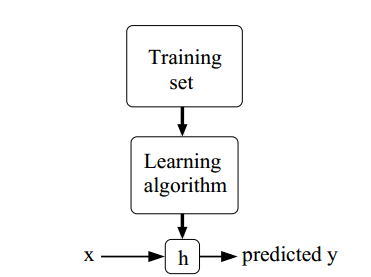
\includegraphics[width=0.5\textwidth]{./figures/machine_learning_diagram}       
\caption{A learning algorithm scheme}
\label{fig:machine_learning_diagram}
\end{figure}

\iftoggle{edit-mode}{\hspace{0pt}\marginpar{HWR Complexity}}{} 
Characters classification is a complex and challenging problems in the pattern recognition field.
This is due to the variation in characters shapes that result from variation in writing habits, styles, and the social and educational level of the writer.
Other factors which implicate the recognition is the variability of writing styles, cursive writing, text size differences and sampling issues, such as duplicate samples resulted from hesitate writers as well as non-adjacent consecutive samples caused by fast writers \cite{verma2004feature}.

\iftoggle{edit-mode}{\hspace{0pt}\marginpar{Letter classification using HMM}}{}
Many types of techniques were investigated for classifying Arabic characters, including Artificial Neural Networks \cite{alijla2012oiahcr}, Decision Trees \cite{ismail2012online}, $k$-NN \cite{elglaly2011isolated} and Hidden Markov Models (HMMs). 
Particularly, HMMs has gained a vast amount of studies done in the field of HWR \cite{pechwitz2003hmm, khorsheed2003recognising, al2007combination, benouareth2008arabic, mahmoud2008recognition, shu1996line, biadsy2006online}. 

While having many advantages, the HMM makes some powerful assumption about the data that may not necessarily true, such as the Markovian assumption which presumes that the transition probabilities depend only on the current state \cite{kadous2002temporal}. 
In addition, HMMs require a large amount of data for its training.

\iftoggle{edit-mode}{\hspace{0pt}\marginpar{The k-NN classifier}}{}
The $k$-nearest neighbours algorithm ($k$-NN) is a well-known classification technique in supervised learning. 
It predicts the query objects class memberships based on the $k$ closest training examples. 
The $k$-NN algorithm is one of the simplest of all machine learning algorithms: an object is classified by a majority vote of its neighbours, with the object being assigned to the class most common amongst its k nearest neighbours ($k$ is a positive integer, typically small). 
If $k=1$, then the object is simply assigned to the class of that single nearest neighbour. 
In many cases, the notion of distance between objects is obvious, however in many other interesting cases it cannot be easily defined.
On the one hand, beside its simplicity, $k$-NN has some major advantages. 
$k$-NN is especially a good learning method for complex target functions.  
On the other hand, the $k$-NN algorithm has some drawbacks. 
First, $k$-NN needs a large dataset in-order to achieve high classification accuracy. 
Second, it is very sensitive to data errors and can be easily fooled by outliers.

\iftoggle{edit-mode}{\hspace{0pt}\marginpar{Literature review}}{}
An on-line Arabic handwritten character recognition method, which uses structural features and decision trees, was presented by Al-Taani and Al-Haj \cite{al2010recognition}. 
The system was tested on a set of 1400 different characters and achieved about 75\% recognition rate. 
The dataset was obtained by capturing the handwriting of 10 users that wrote the 28 Arabic characters, in their isolated form, five times in order.
A rules based approach for on-line Arabic characters classification was proposed in \cite{ismail1859online}. 
The performance of the system was compared to the classification results obtained using artificial neural networks and and decision trees. 
A set of 504 characters were used for training and the test set contained 336 characters. 
The system obtained a recognition rate of about 97\%. 
Addakiri and Bahaj \cite{addakiri2012line} presented an on-line Arabic handwritten character
recognition system based on Neural Networks. 
Their approach was tested on 1400 different characters written by 10 users and achieved accuracy of 83\%.

\subsection{Arabic Script Segmentation}
\iftoggle{edit-mode}{\hspace{0pt}\marginpar{Introduction}}{}
An integral part of the handwriting recognition process, when the analytic approach is considered, is segmentation. 
Therefore, it has long been a critical area of the OCR process. 
As for many pattern recognition problems, the task of segmentation, while usually trivial to a human to perform, is a very challenging pattern recognition problem.
Segmentation and recognition of cursive text are two tasks intertwined and dependent on each other. 
It is believed that wrong segmentation will often result in a major contribution to the error of the recognition algorithm \cite{brodowska2011oversegmentation}. 
But, in order to determine the segmentation, the system may try to seek a pattern that will match a member of the system's alphabet \cite{casey1996survey}.
The segmentation task of cursive and unconstrained nature of languages such as Arabic, makes the segmentation task even harder.  
Several segmentation approaches have been proposed in the literature for Arabic OCR, yet, correct and efficient segmentation of the Arabic text is not easily achievable and considered to be a challenging problem even for printed text. 

\iftoggle{edit-mode}{\hspace{0pt}\marginpar{The context dependent of segmentation}}{}
A reliable recognition system requires more than a good matching to a set of letters symbol classes.
The segmentation decision is not a local decision and may affect subsequent segmentation decisions, thus, a poor match of the current segment to some class in the letter library can cast doubt on the correctness of the future segmentation decisions.
In addition, even a series of satisfactory pattern matches can be judged incorrect if contextual requirements of the system output are not satisfied \cite{casey1996survey}.
For instance, in handwritten English, the letter combination "cl" is graphically similar to the letter "d", but in some cases contextually not valid.
In Arabic, two or three consequent appearances of rasm \RL{-b-} /b/ (that is common for the letters \RL{-y-} /y/, \RL{-t-} /t/ and more, see Section \ref{subsubsec:arabic_writing_characteristic}) are very similar to the \RL{-s-} /s/ letter. 
The only way to distinguish between the two options is by considering the delayed strokes and the contextual validity.

\iftoggle{edit-mode}{\hspace{0pt}\marginpar{Approaches for segmentation}}{}
In a comprehensive survey done in \cite{casey1996survey}, the authors pinpointed two elemental strategies for off-line cursive text segmentation in addition to many approaches that are combinations of these three. 
They have noted that much of the literature on segmentation reports methods that can be characterized as a blend of these three mentioned methods.

\iftoggle{edit-mode}{\hspace{0pt}\marginpar{Dissection}}{}
The first strategy is the classical approach, which is usually named \emph{dissection}, attempts are made to segment the text into primitives. 
Dissection techniques attempt to find appropriate candidate points by learning the characteristic of the segmentation point or by using a rules-based engine. 
Segments, that result from the segmentation process, do not necessarily correspond to exactly one character. 
The word could be segmented into components called graphemes, which are a combination of two or three letters, or a part of a letter. 
The relationship between graphemes and letters is applied in a later phase. 
Many morphological properties were exploited for this task, such as, height, width, separation from neighboring components, low slope if the candidate point local environment, etc.
Various strategies such as projection profile, bounding box or contour tracing exhibit promising results. 
Different types of scripts with essential distinctive nature usually require using different type of properties.
For instance, local minima in the upper or lower contour is commonly used for segmenting English cursive script but not in the Arabic script. 
Such approaches can segment typical words accurately, but, might lead to incorrect segmentation when deal with unconstrained cursive handwriting \cite{saba2010survey}.
A common approach that is followed by many researchers is first over-segmenting of the text, i.e, finding some set of potential splitting points that partition the handwritten word into primitives and then be processed further to eliminate improper candidates point \cite{daifallah2009recognition}.

\iftoggle{edit-mode}{\hspace{0pt}\marginpar{Recognition-based segmentation}}{}
The second approach is the recognition-based segmentation, in which the system searches for sub-components in the cursive text that match letters in its alphabet. 
As mentioned before, character segmentation and character classification are not totally separate steps with a varying degree of dependency.
The initial selection of points can be made in a variety of methods. 
For example, using a moving window with a predefined width which breaks the word into many overlapping pieces without regard to its content.
Then, an iterative or parallel recognition method is used to search for "satisfactory" classification scoring for joint sub-components usually by generating a lattice of all or many possible combinations of the initial candidates set. 
The final decision is determined by the best path through the lattice. 
While avoiding using complex dissection methods, such techniques rely heavily on the classifier accuracy which heavily affects the overall segmentation accuracy \cite{casey1996survey}.

\iftoggle{edit-mode}{\hspace{0pt}\marginpar{Literature Review}}{}
Randa et al. \cite{elanwar2012unconstrained} proposed a two stage on-line Arabic handwritten text segmentation system based on Hidden Markov Model (HMM). 
In the first stage, SPs were nominated, and then, in a second stage, the nominated points were validated using a rules-based engine. 
The system was tested using a self-collected database named OHASD.
Segmentation-based recognition approach based on dividing the word into smaller pieces was proposed in \cite{dinge2011offine}. 
The words were afterwards segmented into candidate letters, and then classified into letter classes, using statistical and structural features. 
A $k$ nearest neighbor ($k$-NN) classifier was used to obtain the final recognition.
A segmentation-based recognition method that operates on the stroke level for on-line Arabic handwritten words recognition was proposed by Daifallah et al. \cite{daifallah2009recognition}. 
SPs were nominated and then selected by locating semi-horizontal lines moving from right to left. 
A portion of the SPs is filtered out by applying a certain set of rules. 
Then, HMM is used to classify the sub-strokes to letters using the Hu feature. 
The letters candidates and their scoring were used to determine the best set of SPs.

%%%%%%%%%%%%%%%%%%%%%%%%%%%%%%%%%%%%%%%%%%%%%%%%%%%%%%%
\newpage{}
%%%%%%%%%%%%%%%%%%%%%%%%%%%%%%%%%%%%%%%%%%%%%%%%%%%%%%%


\section{Thesis Scope and Outline}

In this thesis, we propose and implement a novel real-time approach for segmenting and recognizing on-line handwritten Arabic script.
In Chapter \ref{chap:characters_classification}, we present a fast technique for Arabic characters classification.
The characters classifier employs state-of-the-art similarity measure and search techniques for fast and accurate classification of characters.

A real-time, stroke level, recognition-based, segmentation technique is detailed in Chapter \ref{chap:strokes_segmentation}.
We present a procedure for nominating segmentation points whilst the stroke is being scribed and proposed algorithms for selecting the final segmentation set of segmentation points.
The results obtained by the classification system and the segmentation process are presented in Chapter \ref{chap:results}.
A summary and planned future work are given in Chapter \ref{chap:summary}. 

The ADAB is a de-facto a standard database providing a large dataset of on-line Arabic handwritten samples.
Extracting letter samples from the ADAB database required us to develop a system that enables a human expert to manually segment word samples and produce an Arabic character sample set that can be used in future research. 
An overview on the manual segmentation system and a description of the resulted characters database is given in Appendix \ref{app:data_collection}.
A brief explanation on wavelets and the wavelet transform is provided in Appendix \ref{app:wavelets}. 

The system is based on assumptions and has limitations.
First, it does not regard additional strokes although they can be used to improve the classification results.
Second, the analysis is performed independently on each stroke thus the system does not handle letters spanned over multiple strokes. 
While this is a reasonable assumption, it is not always true. 
Our future work will focus on waiving these limitations. 

%%%%%%%%%%%%%%%%%%%%%%%%%%%%%%%%%%%%%%%%%%%%%%%%%%%%%%%
\newpage{}
%%%%%%%%%%%%%%%%%%%%%%%%%%%%%%%%%%%%%%%%%%%%%%%%%%%%%%%

\section{Conference Publications}

The results of this research have been concluded and published in two conference papers.  

\begin{itemize}

\item A paper titled \emph{"Fast Classification of Handwritten On-line Arabic Characters"} was accepted for publication in the proceedings of the \emph{6th International Conference of Soft Computing and Pattern Recognition} (SoCPaR 2014) in June 20, 2014.

\item A conference paper titled \emph{"Real-time Segmentation of On-line Handwritten Arabic Script"} was accepted for publication in the proceedings of the \emph{14th International Conference on Frontiers in Handwriting Recognition} (ICFHR-2014) in April 21, 2014.

\end{itemize}



%\bibliographystyle{plainnat}
%\bibliography{references}
%\end{document}

%%%% LyX 2.0.5.1 created this file.  For more info, see http://www.lyx.org/.
%%% Do not edit unless you really know what you are doing.
%\documentclass[twoside,english]{report}
%\usepackage[T1]{fontenc}
%\usepackage[latin9]{inputenc}
%\setcounter{secnumdepth}{3}
%\setcounter{tocdepth}{3}
%\usepackage[active]{srcltx}
%\usepackage{verbatim}
%\usepackage{graphicx}
%\usepackage{setspace}
%\usepackage[numbers]{natbib}
%\doublespacing
%
%\makeatletter
%
%%%%%%%%%%%%%%%%%%%%%%%%%%%%%%% LyX specific LaTeX commands.
%\providecommand{\LyX}{L\kern-.1667em\lower.25em\hbox{Y}\kern-.125emX\@}
%%% Because html converters don't know tabularnewline
%\providecommand{\tabularnewline}{\\}
%
%\makeatother
%
%\usepackage{babel}
%\begin{document}

\chapter{Literature Review}
Automated recognition of text has been an active subject of research since the early days of computers. A 1972 survey cites nearly 130 works on the subject \cite{harmon1972automatic}. Despite the age of the subject, it remains one of the most challenging and exciting areas of research in computer science. In recent years it has grown into a mature discipline, producing a huge body of work.
Despite long standing predictions that handwriting, and even paper itself, would become obsolete in the age of the digital computer, both persist. Whilst the computer has hugely simplified the process of producing printed documents, the convenience of a pen and paper still makes it the natural medium for many important tasks.
A brief survey of students in any lecture theater will confirm the dominance of handwritten notes over those typing on laptops. However, the ease and convenience of having information in digital form provides a powerful incentive to find a way of quickly converting handwritten text into its digital equivalent.
The field of handwriting recognition can be split into two different approaches. The first of these, on-line, deals with the recognition of handwriting captured by a tablet or similar touch-sensitive device, and uses the digitized trace of the pen to recognize the symbol. In this instance the recognizer will have access to the x and y coordinates as a function of time, and thus has temporal information about how the symbol was formed. The second approach concentrates on the recognition of handwriting in the form of an image, and is termed off-line. In this instance only the completed character or word is available. It is this off-line approach that will be taken in this report.

{\color{blue}Printed Arabic text is like handwritten Latin text, such that connection of characters is an inherent property for Arabic script whether it is typed, printed or handwritten. Most of errors and deficiencies of Arabic recognition systems comes from the segmentation stages Various segmentation algorithms have been proposed in the literature. Given the vast number of papers published on OCR, it is impossible to include all the segmentation methods in this survey. (Zidouri, Sarfraz, Shahab, \& Jafri, 2005)}

\emph{Need to decide about what to write in this section. Should it contain literature review about every stage in the system? i.e. Pre-processing, segmentation, letters recognition, and post-processing.}

\section{Arabic On-line Recognition Approaches}

\subsection{The Analytic Approach}
\cite{burrow2004arabic}

\subsection{The Holistic Approach}
\cite{burrow2004arabic}

\section{Arabic Text Segmentation}
\emph{copy paste from the paper}

\section{English On-line handwriting Recognition}

%\end{document}


%% LyX 2.0.5.1 created this file.  For more info, see http://www.lyx.org/.
%% Do not edit unless you really know what you are doing.
%\documentclass[12pt,english]{report}
%\usepackage{mathptmx}
%\renewcommand{\familydefault}{\rmdefault}
%\usepackage[T1]{fontenc}
%\usepackage[latin9]{inputenc}
%\usepackage[a4paper]{geometry}
%\setcounter{secnumdepth}{2} % Changed from 3 to 2. 0-chapter 1-section 2-subsection 
%\setcounter{tocdepth}{2} % Changed from 3 to 2. 0-chapter 1-section 2-subsection 
%\setlength{\parskip}{\medskipamount}
%\setlength{\parindent}{0pt}
%\usepackage{verbatim}
%\usepackage{pdfpages}
%\usepackage{graphicx}
%\usepackage{subfig} %% This package has to be here
%\usepackage{setspace}
%\usepackage{arabtex}
%\usepackage[numbers]{natbib}
%\usepackage{nomencl}
%\usepackage{amsthm}
%\usepackage{amsmath}
%\usepackage{amsfonts}
%\usepackage{paralist}
%\usepackage{etoolbox}
%\newtoggle{edit-mode}
%\toggletrue{edit-mode}  
%%%\toggletrue{edit-mode}
%\iftoggle{edit-mode}{
%\geometry{verbose,tmargin=2cm,bmargin=2cm,lmargin=2cm,rmargin=6cm,headheight=1cm,headsep=1cm,footskip=1cm, marginparwidth=5cm}
%}{
%\geometry{verbose,tmargin=2cm,bmargin=2cm,lmargin=2cm,rmargin=2cm,headheight=1cm,headsep=1cm,footskip=1cm}
%}
%
%\makenomenclature
%
%%% Theorem Styles
%\newtheorem{theorem}{Theorem}[section]
%%% Definition Styles
%\theoremstyle{definition}
%\newtheorem{definition}{Definition}[section]
%\newtheorem{example}{Example}[section]
%\theoremstyle{remark}
%\newtheorem{remark}{Remark}
%
%\usepackage[linesnumbered]{algorithm2e}
%
%\begin{document}

\chapter{Data Collection and Preparation}
\label{app:data_collection}

\section{The ADAB Database}
\label{sec:adab_database}

\iftoggle{edit-mode}{\hspace{0pt}\marginpar{The data importance}}{}
The data, its quality and quantity, are a fundamental part of any supervised machine learning technique.
It is used in the learning, validation and testing stages of the pattern recognition process, and has a critical effect on the system accuracy and performance.

\iftoggle{edit-mode}{\hspace{0pt}\marginpar{Data representation}}{}
On-line handwritten data is commonly a digitized representation of the pen movement. 
It may contain sequential information about position, velocity, acceleration, pressure, or even angle and orientation of the pen as a function of time. 
Nevertheless, the pen's position is the most commonly used property. 
Although the sampling of the pen position is done in a constant time intervals, the vast majority of HWR system do not use the temporal information but only consider the serial ordering of pen planar position. 

\iftoggle{edit-mode}{\hspace{0pt}\marginpar{Lack of databases}}{}
Many databases were developed for both on-line and off-line HWR of English script. 
Among these we can mention the following popular database: UNIPEN \cite{guyon1994unipen}, CEDAR \cite{hull1994database}, IRONOFF \cite{viard1999ireste} and NIST.
However, very few databases were developed for the Arabic script and are publicly available such as IFN/ENIT \cite{pechwitz2002ifn} and CEDAR \cite{srihari2005search}.
Thus, most researchers had developed their own private limited datasets \cite{saabni2009efficient}. 
Even fewer datasets were created for the on-line Arabic script. 
This shortage may be attributed to the fact that the major work done on Arabic handwriting recognition focused on recognizing off-line script \cite{plamondon2000online}.
Another reason may be the fact that most research in the on-line script recognition field is done for isolated characters such as letters, digits and symbols \cite{al2011online}.

\iftoggle{edit-mode}{\hspace{0pt}\marginpar{The ADAB database}}{}
In this work, we have used the only publicly available corpus of on-line Arabic handwriting, called the \emph{ADAB} (Arabic DAtaBase) database, which is de-facto a standard in this field \cite{el2009icdar}.
It was developed to advance the research and development of Arabic on-line handwritten text recognition systems and consists of more than 20k Arabic handwritten words scribed by more than 170 different writers.
The samples are words that were taken from the 937 Tunisian town/village names.
Each stroke, represented as a node in the XML, contains the sequence of $(x,y)$ coordinates of the pen position expanded from the pen-down to the corresponding pen-up event, as can be seen in Figure \ref{fig:adab_inkml}.
In addition to the strokes positional information of the stroke, the database contains several properties related to the equipment used to obtain the data and the writer's information, as well as the plot image of the word trajectory as shown in Figure \ref{fig:sample_parts}.

\begin{figure}
\centering
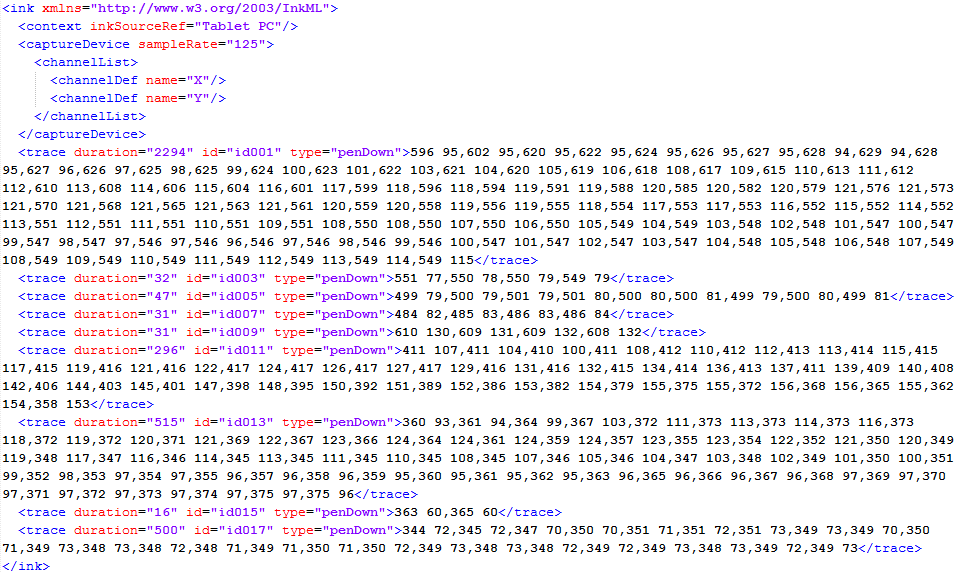
\includegraphics[width=1\textwidth]{./figures/adab_inkml}
\caption{Trajectory information of a city name sample.}
\label{fig:adab_inkml}
\end{figure}

\begin{figure}
\centering
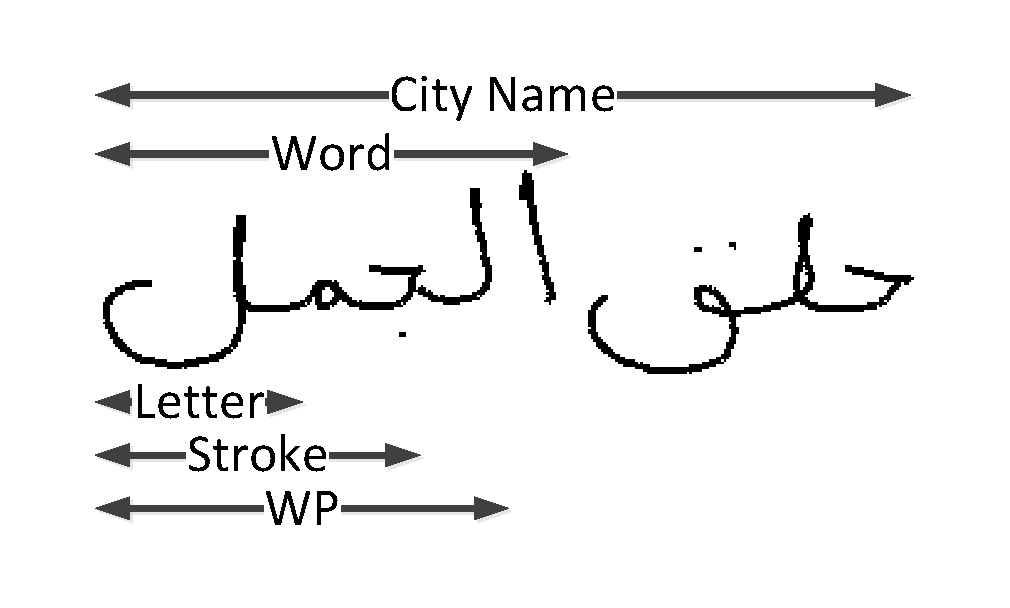
\includegraphics[width=0.4\textwidth]{./figures/sample_parts}
\caption{Visual demonstration of a test sample parts.}
\label{fig:sample_parts}
\end{figure}

%%%%%%%%%%%%%%%%%%%%%%%%%%%%%%%%%%%%%%%%%%%%%%%%%%%%%%%
\newpage{}
%%%%%%%%%%%%%%%%%%%%%%%%%%%%%%%%%%%%%%%%%%%%%%%%%%%%%%%

\section{Letter Samples Extraction}
\label{sec:letters_extraction}

\iftoggle{edit-mode}{\hspace{0pt}\marginpar{The missing information}}{}
The goal of this stage was to create a sufficiently large database of handwritten Arabic letters to be used by the letter classifier described in Chapter \ref{chap:classification}, and as a ground-truth for validating the segmentation method described in Chapter \ref{chap:segmentation}.
The absence of mapping between the strokes and letters in the ADAB database, required manual segmentation of the strokes trajectories.

\iftoggle{edit-mode}{\hspace{0pt}\marginpar{Letters extraction method}}{}
To facilitate the database construction, we have created a user friendly system that reads the samples from the ADAB database, displays the different strokes of a sample in different color, and enables a human expert to easily mark the segmentation points on the strokes.
Once the segmentation process is done, the match between the sub-strokes and the letters is performed in a semi-automatic manner, which required the expert intervention only in cases of ambiguity.  
The system was designed also to handle samples that included more than a single letter. 
In this case, the expert also had to relate the strokes to the different words.
The graphical user interface of the system is shown in Figure \ref{fig:manual_segmentation}. 

\begin{figure}[h]
\centering
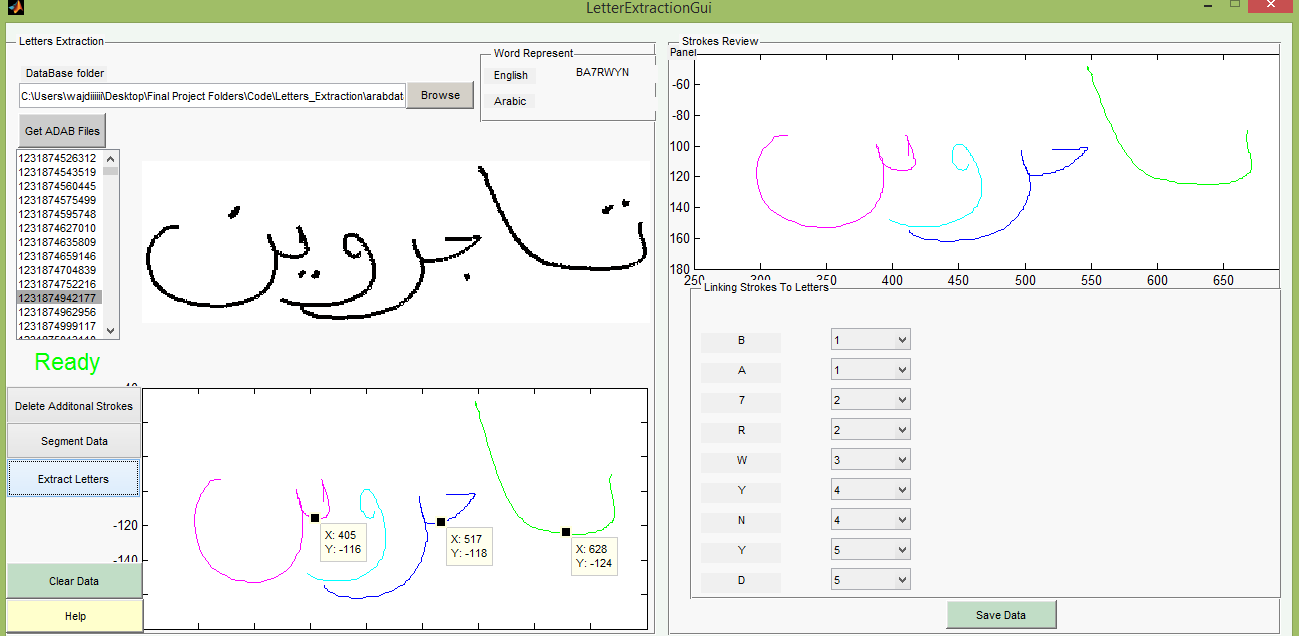
\includegraphics[width=1\textwidth]{./figures/manual_segmentation}
\caption{A view of manual segmentation system.}
\label{fig:manual_segmentation}
\end{figure}

\iftoggle{edit-mode}{\hspace{0pt}\marginpar{Additional strokes detection and removal}}{}
Since, neither the classification system nor the segmentation process consider the additional strokes, the system automatically filtered them out. 
The detection of delayed strokes was performed based on the stroke size and the area of its bounding box. 
However, in order to avoid unintentionally removing main bodies of small letters, we set a relatively high threshold.
Thus, the human expert had to filter out additional strokes manually that could not be identified by the system as such.

\iftoggle{edit-mode}{\hspace{0pt}\marginpar{The output structure}}{}
The output of the system was saved in a parsed XML file for each sample. 
As can be seen in Figure \ref{fig:adab_segmented_xml}, the hierarchy of the out XML represents the structure of the sample as defined in Figure \ref{fig:sample_parts}. 
In order to build up the letters database, an automatic procedure was implemented to extract the letters trajectories from the output XML. 
The letters database consists of directories that represent the different letters.
Each letter directory contains four folders, named Iso, Mid, Fin and Iso which contains the corresponding letter samples, recorded in a Matlab data files.
In the case of a dis-connective letter, the letter folder contains two directories representing the Iso and Mid forms of the corresponding letter.
For the sake of obtaining a sample-set sufficiently large to be used for both learning and validation, more than 7k samples were manually segmented which consisted of about 20k letters. 

\begin{figure}
\centering
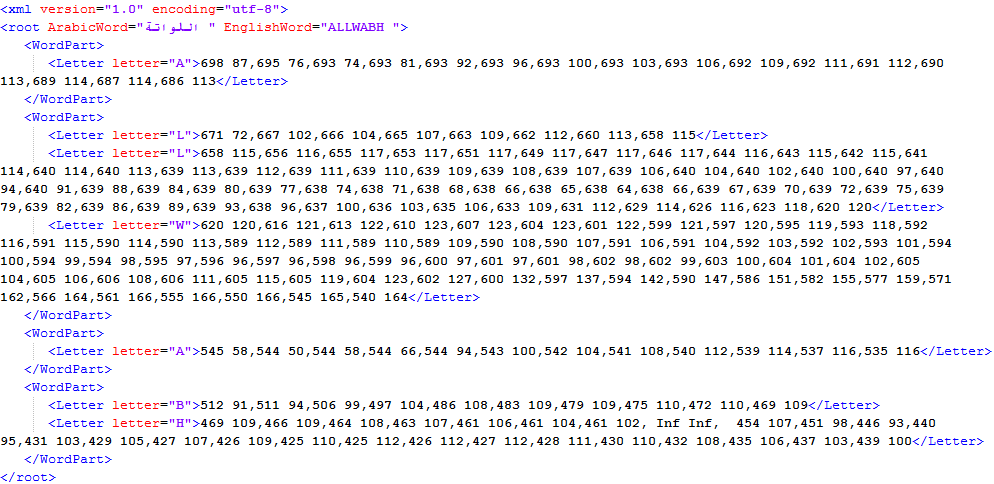
\includegraphics[width=1\textwidth]{./figures/adab_segmented_xml}
\caption{The output parsed  XML.}
\label{fig:adab_segmented_xml}
\end{figure}

%\bibliographystyle{plainnat}
%\bibliography{references}
%\end{document}

%\begin{itemize}
%\item mention that the number of samples per class is different from letter to letter
%\item see "Removing delayed strokes" section in \cite{jaeger2001online}
%\end{itemize}


%% LyX 2.0.5.1 created this file.  For more info, see http://www.lyx.org/.
%% Do not edit unless you really know what you are doing.
%\documentclass[12pt,english]{report}
%\usepackage{mathptmx}
%\renewcommand{\familydefault}{\rmdefault}
%\usepackage[T1]{fontenc}
%\usepackage[latin9]{inputenc}
%\usepackage[a4paper]{geometry}
%\setcounter{secnumdepth}{2} % Changed from 3 to 2. 0-chapter 1-section 2-subsection 
%\setcounter{tocdepth}{2} % Changed from 3 to 2. 0-chapter 1-section 2-subsection 
%\setlength{\parskip}{\medskipamount}
%\setlength{\parindent}{0pt}
%\usepackage{verbatim}
%\usepackage{pdfpages}
%\usepackage{graphicx}
%\usepackage{subfig} %% This package has to be here
%\usepackage{setspace}
%\usepackage{arabtex}
%\usepackage[numbers]{natbib}
%\usepackage{nomencl}
%\usepackage{amsthm}
%\usepackage{amsmath}
%\usepackage{amsfonts}
%\usepackage{etoolbox}
%\newtoggle{edit-mode}
%\togglefalse{edit-mode}  
%\toggletrue{edit-mode}
%\iftoggle{edit-mode}{
%\geometry{verbose,tmargin=2cm,bmargin=2cm,lmargin=2cm,rmargin=6cm,headheight=1cm,headsep=1cm,footskip=1cm, marginparwidth=5cm}
%}{
%\geometry{verbose,tmargin=2cm,bmargin=2cm,lmargin=2cm,rmargin=2cm,headheight=1cm,headsep=1cm,footskip=1cm}
%}
%
%\makenomenclature
%
% Theorem Styles
%\newtheorem{theorem}{Theorem}[section]
% Definition Styles
%\theoremstyle{definition}
%\newtheorem{definition}{Definition}[section]
%\newtheorem{example}{Example}[section]
%\theoremstyle{remark}
%\newtheorem{remark}{Remark}
%
%\usepackage[linesnumbered]{algorithm2e}
%
%\begin{document}
%\printnomenclature{}
%
%\tableofcontents{}

\chapter{Handwritten Arabic Letters Classifier}

\section{Introduction}

\iftoggle{edit-mode}{\hspace{0pt}\marginpar{Complexity of the Arabic handwriting recognition}}{}
On-line handwriting recognition is one of the very complex and challenging problems in the pattern recognition field due to the variability of writing styles, cursive writing, text size differences and sampling issues caused by duplicate samples resulted from hesitate writers as well as non-adjacent consecutive samples caused by fast writers \cite{verma2004feature}. The problem that makes the recognition of on-line handwriting recognition difficult is variation of shapes of the characters resulting from writing habits, styles, and the social and educational level of the writer.
%Correct and precise classification is a fundamental part of any \emph{Optical character recognition} (OCR) system.
In this chapter we will discuss theoretical aspect as well as implementation details of the classification engine implemented in our system. \emph{TODO: fix this paragraph}\\ 

\iftoggle{edit-mode}{\hspace{0pt}\marginpar{Input-output}}{}
Given a stroke sequence, and a position as an input parameter to the classifier, it produces a list of candidate samples from the sample set which are most similar to the given sequence, with a scoring attached to each candidate. Thus, actually, the classifier contains four databases. On for each letter position. This partitioning of the samples to four database, clearly, improve the classification power and the accuracy of the classification and scoring.\\

\iftoggle{edit-mode}{\hspace{0pt}\marginpar{Performance}}{}
The performance of the on-line classifier is a crucial property of the 
needed classifier since, as mentioned in the overview in chapter \ref{}, the goal of the system is to perform strokes segmentation and letters recognition while the stroke is being written.\\ 

\iftoggle{edit-mode}{\hspace{0pt}\marginpar{Constructs classification}}{}
In the on-line text recognition, the classification can be done in several levels. The Recognition system can be built to classify an entire words, Word-parts, letters or even strokes. In this work we chose to work with strokes, since it represent the most basic element a writer can produce after the point, and it contains in most cases a single letter or more.\\

\iftoggle{edit-mode}{\hspace{0pt}\marginpar{Talk in general about the technique we use - mention each stage in general}}{}
Text Recognition can be broken down into three main stages: \emph{preprocessing}, \emph{feature extraction} and \emph{classification}. The preprocessing stage usually consists of normalization, re-sampling, noise elimination and smoothing steps to give the a uniform structure and avoid irrelevant information that can negatively affect the recognition. In the feature extraction stage, important information in the data is highlighted and represented as vectors in the feature space which is used by the classifier. The last important step is classification, which identify the class for which the sample belong.\\

%We will start our discussion by giving the required background to pattern recognition, in general, and to the handwritten text recognition field in particular.\\

%\iftoggle{edit-mode}{\hspace{0pt}\marginpar{Types of learning problems.}}{}
%Machine learning is a branch in computer science of getting computers to act without being explicitly programmed. 
%The are mainly three types of learning: supervised, unsupervised and reinforcement learning.
%In the supervised learning, as seen above, a set of classified samples is given. In the unsupervised learning case, unlabeled data is given and the goal is to find a hidden structure in it. The reinforcement learning is a type of learning inspired by behaviorist psychology, concerned with how software agents ought to take actions in an environment so as to maximize some notion of cumulative reward. The handwriting recognition in most of it's implementation is a supervised learning problem.\\

\iftoggle{edit-mode}{\hspace{0pt}\marginpar{The learning problem.}}{}
In \emph{supervised learning}, classification is the problem of identifying to which of a set of classes a new observation belongs. It is done on the basis of a training set of data containing instances for which the their class membership is known.
Formally, the supervised learning problem is defined as follows:
\begin{definition}
Given a domain space $X$, a target space $Y$ and a training set $S=\{(x_i,y_i)\}_{i=1}^{m}$ where $x_1,x_2,..,x_n\in X$ and $y_1,y_2,...,y_n \in Y$. Let us assume that there is an unknown target function $f$ for which $f : X\rightarrow Y$. A Learning algorithm $A$ produces hypothesis function $h$ based on $S$ such that $h \approx f$, i.e., the function $h$ is an approximation for the target function $f$ and $h \in H$, the hypotheses set. 
\end{definition}

\begin{figure}
\centering
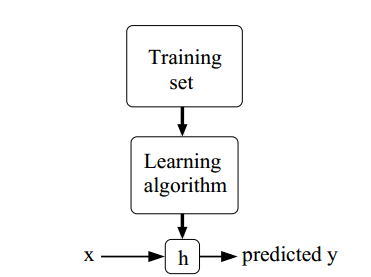
\includegraphics[width=0.5\textwidth]{./figures/machine_learning_diagram}       
\caption{A learning algorithm scheme}
\label{fig:machine_learning_diagram}
\end{figure}

\iftoggle{edit-mode}{\hspace{0pt}\marginpar{The classification problem}}{}
In many cases, the learning problem is actually a classification problem. For any given classification problem, there is an intuitive belief that there exist a space to which the samples can be transformed and in which can be portioned into regions that represent categories. Accordingly, the problem of classification is basically the problem of portioning the sample space into regions. Having done that, classifying a new unlabeled observation is done by determining the partition it belongs to. Ideally, one would like to arrange this partitioning so that none of the decisions is ever wrong. When this cannot be done, one would like to minimize the probability of error \cite{duda1973pattern}.

\iftoggle{edit-mode}{\hspace{0pt}\marginpar{What we actually try to do? and How?}}{}
Since no such partition on the raw data space is known. We try to find the mentioned space in the feature space and to approximate the mentioned partitioning.
 \emph{TODO: describe what each step do in a high level.}

\iftoggle{edit-mode}{\hspace{0pt}\marginpar{Types of approaches in the supervised Learning.}}{}
%In machine learning, pattern recognition is the assignment of a label to a given input value. 
Many supervised learning approaches and algorithms were proposed to solve the classification problem. Decision trees, artificial neural networks, support vector machines, Bayesian networks and nearest neighbor are few well-known learning techniques. A review on the supervised classification algorithms is given by Mohamed Aly in \cite{aly2005survey}.The role of the machine learning specialist is to identify the type of the learning problem and meet the needs of the problem by stitching the best solution for it. The classification process is usually contains several steps. These preliminary steps include normalization, noise removal, feature extraction, dimensionality reduction, etc. emph{[fix]}\\


\iftoggle{edit-mode}{\hspace{0pt}\marginpar{Classification techniques in HW recognition}}{}
Different approaches were considered to solve the text recognition problem. Each has it's advantages and drawbacks, and each is suitable for a certain system requirements and implementation.
The classification algorithm used in the recognition process is the most central stage. All the preprocessing stages prepare the data for the classification stage. The classification stage may be composed of more than a single stage.  
In the following, we will mention the few most common approaches commonly used for letters classification and discuss their advantages and drawbacks.\\

\iftoggle{edit-mode}{\hspace{0pt}\marginpar{HMM - An introduction}}{}
Unlike in the off-line case, on-line handwriting can be viewed as temporal series, therefore many pattern recognition techniques from the temporal information field were adopted for handwriting recognition. One example is the  \emph{hidden Markov models} (HMM). HMM is an extension of the discrete-state Markov process. \emph{TODO: give some more information about the theory of HMM}

\iftoggle{edit-mode}{\hspace{0pt}\marginpar{HMM for online handwriting recognition}}{}
There is a vast amount of studies done in the field of handwriting recognition field that use HMM \cite{pechwitz2003hmm, khorsheed2003recognising, al2007combination, benouareth2008arabic, mahmoud2008recognition, shu1996line}. 
Letters, words and sentences can be modeled using HMM and using the solution of the learning problem, letter words and sentences can be identified. Reader unfamiliar with this approach, a good introduction on using HMM for time series classification in general and text recognition in particular can be found \cite{kadous2002temporal, shu1996line}.\\ 

\iftoggle{edit-mode}{\hspace{0pt}\marginpar{HMM - disadvantages}}{}
While having many advantages, there are some drawback of using HMM, Kondous has pointed out in his Ph.D Thesis \cite{kadous2002temporal}. First, it makes powerful assumption about the data that may not necessarily true. One example is the Markovian assumption, i.e., that the transition probabilities depend only on the current state. Second, there is no specific way to determine the number of states, thus intelligent guesses and try and error are usually employed. Furthermore, the states and transitions depend on the class being learned. For example, is there any reason why the words "dog" and "butterfly" would have similar states and transitions? Third, HMM requires a very large amount of data for its training.\\

\iftoggle{edit-mode}{\hspace{0pt}\marginpar{Artificial Neural Networks - an introduction}}{}
Artificial neural network is also a widely used technique for letters recognition. It is a generalization of linear discrimination. 

\iftoggle{edit-mode}{\hspace{0pt}\marginpar{ANN - drawbacks}}{}


\iftoggle{edit-mode}{\hspace{0pt}\marginpar{k-NN classifier in general}}{}
The k-nearest neighbors algorithm ($k$-NN) is a well-known classification technique in supervised learning. It predicts the query objects class memberships based on the k closest training examples. The k-nearest neighbor algorithm is one of the simplest of all machine learning algorithms: an object is classified by a majority vote of its neighbors, with the object being assigned to the class most common amongst its k nearest neighbors (k is a positive integer, typically small). If $k=1$, then the object is simply assigned to the class of that single nearest neighbor. In many cases the notion of similarity between sample object is obvious, however in many other interesting cases the distance between objects cannot be easily defined.
Beside its simplicity, $k$-NN has some major advantages. First, $k$-NN is a good learning method for complex target functions. Second, it is easy to implement. Third, arbitrary objects similarity function can be applied easily.\\

\iftoggle{edit-mode}{\hspace{0pt}\marginpar{Advantages and Downside of the $k$-NN classifier}}{}
$k$-NN algorithm has dome drawbacks that reader needs to note. $k$-NN needs a large data set in-order to achieve high classification accuracy. Another drawback is that it is very sensitive to data errors and can be easily fooled by outliers.\\

\iftoggle{edit-mode}{\hspace{0pt}\marginpar{Scoring-based NN classification}}{}
Several machine learning problems, especially those having a large number of classes, the classifier, returns a set of potential candidate classes or even specific samples in the. In these cases, for each candidate class, the classifier usually gives a scoring that can be used by a later part in the classification process (e.g. in the post processing). Such approach is taken for objects classification in our system. sample set that are closely resembles a given unknown sample. This approach can be used for both supervised and unsupervised learning domain. In the supervised learning case since the classification of the returned samples is known, the hypothesis function, classifies the inputed sample based of candidate labels.\\

\iftoggle{edit-mode}{\hspace{0pt}\marginpar{Why did we use the NN as a classifier}}{}
For the disadvantages for HMM and NN techniques mentioned above and the intuitive and simplicity of the and for my personal interest in similarity measure techniques that can be integrated classifier, we have chosen to use Nearest Neighbor classifier classification.\\ 

\iftoggle{edit-mode}{\hspace{0pt}\marginpar{NN classification}}{}
In the $k$-NN problem a set of data points in d-dimensional space is given and for a query point q, the nearest or generally k nearest points of P to q can be reported efficiently. The distance between two points can be defined in many ways as will be detailed in Section \ref{[]}. $k$-NN based classification a very basic and common approach for implementing the pattern classification. However, the retrieval of the exact k-Nearest Neighbors for a given query object $q$ and a database of sample set $S$ suffers from bad performance that is mainly caused by two factors. The first, is the total numbers of samples in the data. This issue will be discussed in Section \ref{sec:similarity_search} and the other is the dimensionality of objects in the data (known as the \emph{curse of dimensionality}). Computing exact nearest neighbors in dimensions much higher than 8 seems to be a very difficult task. However, the first issue has much smaller impact on the speed of the nearest neighbor retrieval and can be healed easily by using dimensionality reduction techniques which will be discussed in details in Section \ref{sec:dimensionality_reduction}. However, the first issue, i.e., the size of the sample data, is crucial. The simplest solution to the NN problem is to linearly go over the entire sample set and keep track of the best k best nominates so far. The running time of this algorithm in $O(Nd)$ where $N$ is the cardinality of sample set and d is the dimensionality of the sample set. While looking in the entire database for the $k$-NN is not permissible for most applications. The only advantage of this approach is that it requires no extra space, beyond the amount of the memory needed for keeping the sample set. This issue is will be treated in Section \ref{similarity_search}. \\

%%%%%%%%%%%%%%%%%%%%%%%%%%%%%%%%%%%%%%%%%%%%%%%%%%%%%%%
\newpage{}
%%%%%%%%%%%%%%%%%%%%%%%%%%%%%%%%%%%%%%%%%%%%%%%%%%%%%%%

\section{Samples Preprocessing}

The data obtained by the digitizer is composed of points in the plane that represent the trajectory scribed by the writing instrument on the tablet surface. Usually, samples are taken in time intervals, thus slow pen motion regions are oversampled and fast motion regions are under-sampled. In addition, when such devices are used to capture handwriting strokes, the shapes of the strokes present a jagged form and the obtained data is non-uniform and noisy. Further imperfections are caused by hand vibrations and duplicated sampled points resulted from hesitant writing. This noise should be reduced as much as possible since it influence the further processes, such as feature extraction and classification \cite{al2011online} \cite{huang2009preprocessing}.  
To overcome the flaws mentioned, preprocessing operations are usually applied. The preprocessing steps imposes certain uniform structure on the data to comply with the input structure required by the latter parts of the system, such that vector length, sequence bounds, etc.\\

\emph{TODO: mention other preprocessing approaches mentioned in the literature, like rotation normalization, slant normalization, and missing points interpolation. see \cite{jaeger2001online}.}

As seen in Figure \ref{[]} and \ref{[]}, preprocessing is performed in both letters learning and classification of strokes.
Preprocessing is also done in the segmentation phase, however, not all steps mentioned in this section are performed. For more information see section \ref{[]}

Data samples must be of the same dimension for the system to work properly. Since the collected letters in the database are of varying sizes, they were all resized to some standard size. and re-sampled to to achieve same length sequences.
Our preprocessing phase include three steps in the following order: \emph{Normalization and Translation}, \emph{Noise Elimination} and then \emph{Smoothing and Re-sampling}.\\ 

In Figure \ref{fig:D_before_after_preprocessing} we show a sample of the letter \RL{d} sequence before and after preprocessing.\\ 

In the next sub-sections we will describe in details each part of the preprocessing procedure.

\begin{figure}
	\centering
        \subfloat[]{
            \label{fig:letter_before_preprocessing}
            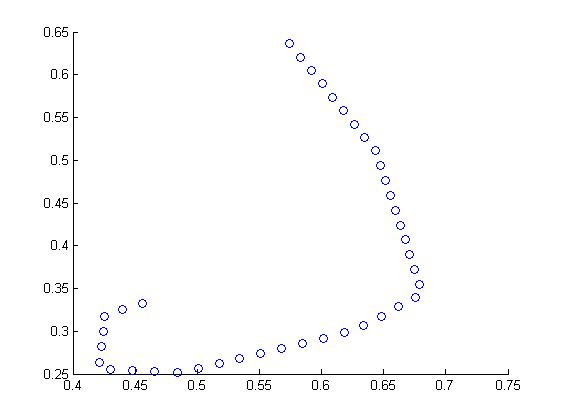
\includegraphics[width=0.5\textwidth]{./figures/letter_before_preprocessing}
        }
        \subfloat[]{
           \label{fig:letter_after_preprocessing}
           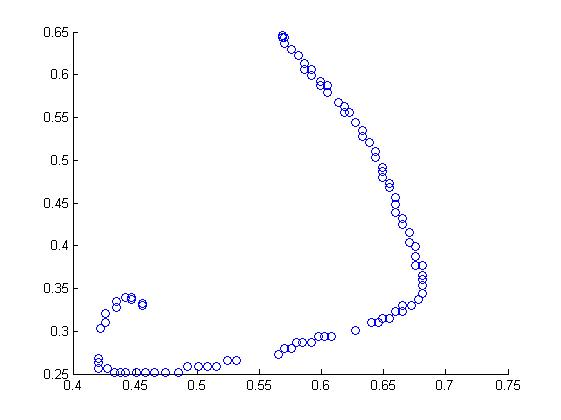
\includegraphics[width=0.5\textwidth]{./figures/letter_after_preprocessing}
        }        
    \caption{The letter \RL{d} before (a) and after (b) preprocessing}
   \label{fig:D_before_after_preprocessing}
\end{figure}

\emph{refer to the slant and Rotation normalization, i.e., why we don't do it. Is slant common in Arabic?
}

\subsection{Normalization and Translation}

Size normalization is done to achieve a uniform size of the bounding box surrounding the pattern. This is done to enable the classifier to recognize the sequence pattern even when the stroke is written in different sizes. Shape similarity algorithms tend to be sensitive for non-uniform shapes size, thus this procedure is important and can be found in many approaches in the literature. 
However, this method could not be applied since normalization is done in our system on the stroke level which could contain a letter, at least.
In our approach size normalization was applied on each stroke such that all strokes have $[0,1]\times[0,1]$ bounding box but retain their original aspect ratio. We include in this step also translation of the sequence's center of gravity to the origin point $[0,0]$.
Given the stroke sequence $S=\{p_i\}_{i=1}^{n}$, the normalized sequence $\bar{S}=\{\bar{p_i}\}_{i=1}^{n}$ is calculated by: 

\begin{equation}
{\bar x_i} = {{\left( {{x_i} - {\mu _x}} \right)} \over W},{\bar y_i} = {{\left( {{y_i} - {\mu _y}} \right)} \over W}
\end{equation}
Where
\begin{equation}
\mu  = \left( {{\mu _x},{\mu _y}} \right) = \left( {{1 \over N}\sum\limits_{i = 1}^N {{x_i}} ,{1 \over N}\sum\limits_{i = 1}^N {{y_i}} } \right)
\end{equation}
\begin{equation}
W = \max \left( {{d_x},{d_y}} \right)
\end{equation}
\begin{equation}
{d_x} = {x_{\max }} - {x_{\min }};\,\,\,{d_y} = {y_{\max }} - {y_{\min }}
\end{equation}
\begin{equation}
{x_{\max }} = \mathop {\max }\limits_i \left( {{x_i}} \right),\,\,{x_{\min }} = \mathop {\min }\limits_i \left( {{x_i}} \right),\,\,{y_{\min }} = \mathop {\min }\limits_i \left( {{y_i}} \right),\,\,{y_{\min }} = \mathop {\min }\limits_i \left( {{y_i}} \right)
\end{equation}  

\subsection{Noise Elimination}
The input obtained by the digitizer may contain a large amount of noise which is mainly duplication of points. In this process redundant points are filtered out and a similar sequence with fewer points is obtained.
In order to eliminate redundant points irrelevant for pattern classification and screening out unwanted noise and vibrations in the letter inscription we have used the \emph{Douglas-Peucker Polyline Simplification algorithm} described in \cite{douglas1973algorithms}. Briefly, it is a line simplification algorithm to reduce the number of vertices in a piecewise linear curve according to a specified tolerance. The algorithm is also known as \emph{Iterative Endpoint Fit}. The resulted curve is a skeletonized angular sequence. The Normalization is done before the Simplification, since we need a constant simplification parameter $\varepsilon$ which was tuned for $1\times1$ bounds. 
Assuming the stroke presentation is a sequence of points $S$, the sensitivity parameter that was used in our work is:
\begin{equation}
\varepsilon  = {1 \over {200}}\sqrt {{d_x}^2 + {d_y}^2}
\end{equation}

\begin{figure}
\centering

\includegraphics[width=0.7\textwidth]{./figures/ha_simplification}       
\caption{Non Simplified representation of the letter \RL{.h} (Ha) is shown on the right. A simplified version is shown on the left. \emph{TODO: change the pictures to something better}}
\label{fig:ha_simplification}
\end{figure}

\subsection{Smoothing and Re-sampling}
As a result of the simplification process the points are not distributed uniformly along the stroke trajectory. Naturally, there are less point in relatively straight areas and a higher amount of points in the curved areas of the stroke.\\ 
%if we wont use simplification we can write this: The re-sampling is needed to prevent the unbalanced sampling density, which may be influenced by the sampling rate and the user non-uniform letter drawing. 
The re-sampling produces equidistant smoothed data sequence. 
The Re-sampling is performed using splines interpolation as follows:\\
Given a stroke $S=\{p_i\}_{i=1}^{n}$ and the re-sampling target number $R$, let $\{X(a_i)\}_{i=1}^{n}$ and $\{Y(a_i)\}_{i=1}^{n}$ represent the x-axis and the y-axis sequences with respect to the parameter $a_i$ which is defined as follows:

\begin{equation}
a_i=a_{i-1}+arclen(p_{i-1},p_i) 
\end{equation}  

\begin{equation}
X(a_i)=x_i 
\end{equation}  

The arc-length of the stroke is given by $L=a_n$.\\

A piecewise linear interpolations $q_X(a)$ and $q_X(a)$ are created for the $X$ sequence and $Y$ sequence respectively.
The breaks are the $a_i$ sequence and the coefficient of the linear polynomial are $\alpha_{i} = \frac{X(a_i)-X(a_{i-1})}{a_{i}-a_{i-1}}$ 

\emph{[we use quadratic splines for smoothing and simplification.]}

let $t_i=i\frac{L}{R}$ for $i=0,...,R$.
The re-sampled sequence is given as follows:
\begin{equation}
\widehat{S}=\{(q_X(t_i),q_Y(t_i))\}_{i=1}^{R}
\end{equation}

The target number of points is set to 40. We had to find a number that is good enough for both long and short strokes since strokes can span over a single letter or a whole WP.

\emph{[TODO: show the following images: 1. the scattered stroke, 2. X and Y as a function of t., 3. X and Y resampledm and 3. the stroke resampled. ]}

\emph{[TODO: talk about splines.]}

\emph{TODO: talk about the other smoothing techniques as described in \cite{jaeger2001online} -- Online handwriting recognition: the NPen++ recognizer}

\subsubsection{Approach 1 - Using piecewise linear interpolations}

\subsubsection{Approach 2 - Using quadratic splines}

\begin{figure}
\centering

\includegraphics{./figures/y_resampling}       
\caption{Representation of a non-resamples sequence of the letter \RL{y} (Y) is shown in the right. The re-sampled version is shown on the left.}
\label{fig:y_resampling}
\end{figure}

Answer the following:
\begin{itemize}
\item Mention that the data in the database was not in the same length therefore normalziation and re-sampling were needed. 
\item Where preprocessing is used in our system? Letters Learning and strokes classification
\item What parameters were used for each preprocessing stage and why.
\item what alternatives were considered.
\end{itemize}

%%%%%%%%%%%%%%%%%%%%%%%%%%%%%%%%%%%%%%%%%%%%%%%%%%%%%%%
\newpage{}
%%%%%%%%%%%%%%%%%%%%%%%%%%%%%%%%%%%%%%%%%%%%%%%%%%%%%%%

\section{Features Extraction}
\label{sec:feature_extraction}

\iftoggle{edit-mode}{\hspace{0pt}\marginpar{Introduction}}{}
Feature extraction is certainly one of the important parts of any pattern classification system and plays an important role in the overall process of handwriting recognition. It aims is to cull informative parameters for learning and recognition of patterns.  Most classification methods require that patterns be represented in a fixed dimensional feature space that is often incompatible with input data. Poor feature extraction and selection will always result in a poor system performance, regardless of the ingeniousness of the learning and classification algorithms \cite{parizeau2001character}.\\

\iftoggle{edit-mode}{\hspace{0pt}\marginpar{Introduction - Cont.}}{}
Feature extraction methods operate differently in different domains and may have slightly different goals in different pattern recognition fields. For instance, in the image retrieval field, the input data (i.e., the image) is too large and suspected to be redundant. In this case, feature extraction techniques are used to reduce the representation of the input data into a compact representation set of features. However, In the shape recognition domain, the input data is compact and feature extraction techniques are used to transform it into feature vectors, which are usually referred to as \emph{shape descriptors}. Shape descriptors offer discriminative characterization to capture the perceptual dissimilarity between two shapes. Unlike the first case, the raw amount of data contained in feature vector usually exceeds the amount of data in the original input data.\\

\iftoggle{edit-mode}{\hspace{0pt}\marginpar{Shape Descriptors}}{}
The goal of a shape descriptor is to be able to effectively find perceptually similar shapes from a database. Shape descriptors are usually in the form of vectors that are produced to represent a given shape feature and attempts to quantify perceptual similarities between shapes. That is to say, shapes which are found perceptually similar by human have resembling descriptor than from shapes that are different from the others. Effective shape descriptor must present some essential properties such as translation, rotation and scale invariance. It also must be as robust as possible against noise so that variously distorted shapes which are tolerated by human beings when comparing shapes should be endured also by the shape descriptor. This is known as the robustness requirement \cite{zhang2004review}.\\

\iftoggle{edit-mode}{\hspace{0pt}\marginpar{Shape Descriptors properties}}{}
The following are properties of a desirable shape descriptor: 1. good retrieval accuracy; 2. compact features; 3. low computation complexity; 4. robust retrieval performance \cite{kim2000region}.\\

\iftoggle{edit-mode}{\hspace{0pt}\marginpar{Shape Descriptors - Handwriting recognition}}{}
Many shape descriptors have been developed in order to improve the segmentation and recognition rates. There are many different classifications and sub-classifications of shape descriptors according to their method of operation. The most common classification is the classification for local and global descriptors. Local descriptors calculate some feature at each sample point. An example for a local feature is the vector that contain the tangent slope angle for every given point in the sample point. \emph{Normalized curvature} and \emph{Ratio of tangent} \cite{hu1995invariant, hu1996hmm} are examples of more complex local shape descriptor. Descriptors such as cusps, crossings and loops are referred to as global descriptors and are calculated on the entire shape \cite{hu1997combining}. For a comprehensive review on shape descriptors see \cite{zhang2004review} and \cite{yang2008survey}.

%\emph{TODO: review "Local vs. global Features" (p. 30) in \cite{connell2000online} }

\iftoggle{edit-mode}{\hspace{0pt}\marginpar{Using off-line shape descriptors for on-line handwriting recognition}}{}
Many of the well known and powerful features operate on the shape's contour. This is because many descriptors were developed for off-line handwriting recognition. However, the input data in the on-line case is a sequence of points and no contour is involved. Using features in on-line handwriting recognition that we originally developed for the off-line case is common. Saabne and El-Sanna employed the \emph{Shape Context} (SC) descriptor, a global shape descriptor that was originally developed for contour based shapes,  on-line handwriting recognition in \cite{saabni2009hierarchical}. Multi Scale shape context is used by Hu and Zanibbi in \cite{husegmenting} for on-line handwritten mathematical expressions segmentation. The original definition of the mentioned features is given on the contour of the shape. However to use it in the on-line writing recognition case, the features are applied upon the stroke sequence.\\ 

\iftoggle{edit-mode}{\hspace{0pt}\marginpar{Selected Descriptors}}{}
In this work we have chosen to work with two shape descriptors, the Shape context descriptor, MAD and  the tangent angle feature. The reason for this choice is that we wanted to investigate how both global and local features effectiveness in our proposed process. More information about these features are given below.\\

\nomenclature{$SC$}{Shape Context Descriptor}
\iftoggle{edit-mode}{\hspace{0pt}\marginpar{Shape Context}}{}
Belongie and Malik have presented a point matching approach named Shape Context \cite{belongie2002shape}. The Shape context is a shape matching approach that intended to be a way of describing shapes that allows for measuring shape similarity and the recovering of point correspondences. This approach is based on the following descriptor: Pick $n$ points on the shape's contour, for each point ${p_i}$ on the shape, consider the $n - 1$ other points and calculate the coarse histogram of the relative coordinates. Equation \ref{eq:sc_bins} is defined to be the shape context of ${p_i}$.

\begin{equation}
{h_i}(k) = \# \{q \ne p_i:(q - p_i) \in bin(k) \}
\label{eq:sc_bins}
\end{equation}

The bins are normally taken to be uniform log-polar space making the descriptor more sensitive to positions of nearby sample points than to those of points farther away. This distribution over relative positions is robust and compact, yet highly discriminative descriptor. The basic Idea of the Shape Context Descriptor is illustrated in Figure \ref{fig:shape_context_demo}. This can be calculated in $O(N^3)$ time using the Hungarian method. \\

\begin{figure}
\centering
\subfloat[]{
    \label{fig:shape_context_offline}
    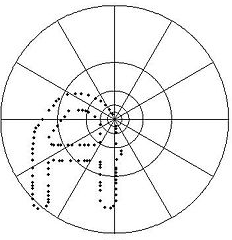
\includegraphics[width=0.27\textwidth]{./figures/shape_context_offline}
}
\subfloat[]{
	\label{fig:shape_context_online}
     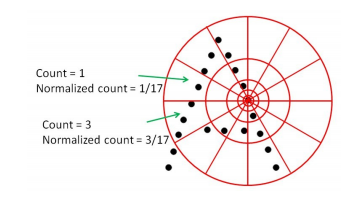
\includegraphics[width=0.3\textwidth]{./figures/shape_context_online}
}        
\caption{Diagram of the log-polar bins used to compute the shape context. On-line and off-line}
\label{fig:shape_context_demo}
\end{figure}

\nomenclature{MAD}{Multi Angular Descriptor}
\iftoggle{edit-mode}{\hspace{0pt}\marginpar{MAD}}{}
The other shape descriptor used in this thesis is the Multi Angular Descriptor (MAD).
MAD was proposed by Saabni in \cite{saabni2013multi}. It captures the angular view to multi resolution rings in different heights. The shape is treated as a two dimensional set of points and the different rings are upper view points from rings around the shape centroid with different sizes and heights. To enables scale and translation invariance, the sizes and heights of these rings are calculated using the diameter and centroid of the shape.
Formally, let $S$ be a shape and Let $C$ and $D$ be the centroid and the diameter of the shape respectively. Let $P = \{p_i\}_{i = 1}^l$ a set of $l$ point taken uniformly from the extracted contour of $S$. Given a view point $V_j$ from a given ring with height $h$ over the shape, the angle, obtained by connecting the point ${p_i} \in P$ with each point   and the plain of the shape is a rich description of the shape from this view point. Let $R$ be a ring with the radius $r$ and the center $C$ positioned above the shape $S$ with the height $h$. Let $V = \{V_i\}_{i = 1}^n$ be a set of $n$ viewpoints lying uniformly on the ring $R$ and $\alpha(V_{ij})$ to be the angle between the segment $\overline {{V_i}{p_j}}$ and the plain contains the shape $S$. The vector $Ve{c_i} = \left\{ {\alpha \left( {{V_{ij}}} \right)} \right\}_{j = 1}^l$ can be seen as watching the shape $S$ from one upper view point $V_i$. Illustration can be seen in Figure \ref{fig:mad_demo}.\\

\begin{figure}
\centering
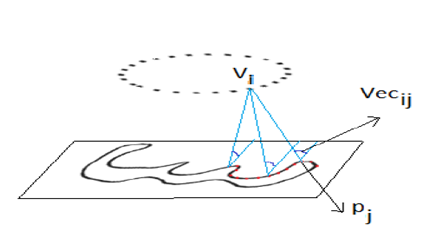
\includegraphics[width=0.5\textwidth]{./figures/mad_demo}       
\caption{An example of three line segments drawn from the same viewpoint $V_i$, generating the three angles $Vec_{ij}$ with the plane of the shape. When the parameter $j$ goes over all contour points we get the vector $Vec_i$ describing the shape from the view point $V_i$ with the parameter $i$ goes over all viewpoints.}
\label{fig:mad_demo}
\end{figure}

\iftoggle{edit-mode}{\hspace{0pt}\marginpar{Results - Asses the quality of separation in the features space}}{}
In order to evaluate the quality of the features we asses the quality of classification. Since as can be seen the coming chapters, our classification is based on Neasrest Neighbors classification, after considering several quality evaluation methods, we selected the following. \emph{TODO: give more information on clusters validation techniques.}
The evaluation is done as follows: First we initialized a scoring parameter to 0, i.e., $s=0$. Then, for each sample in the sample set, the closest three candidates are extracted and ordered by their vicinity to the sample element. The distance function that is used here is the Euclidean distance. Let us denote the correct sample labeling by $a$ and the labeling of the candidates by $\alpha, \beta, \gamma$ respectively. If $\alpha=a$ then we do $s=s+3$. If $\beta=a$ then we do $s=s+2$. If $\gamma=a$ we perform $s=s+1$.
The scoring is then calculated as follows: $S=\frac{s}{6N}$, where the $N$ is the size of the sample set.

%%%%%%%%%%%%%%%%%%%%%%%%%%%%%%%%%%%%%%%%%%%%%%%%%%%%%%%
\newpage{}
%%%%%%%%%%%%%%%%%%%%%%%%%%%%%%%%%%%%%%%%%%%%%%%%%%%%%%%

\section{Similarity Measures}
\label{sec:similarity_measures}

\iftoggle{edit-mode}{\hspace{0pt}\marginpar{Introduction}}{}
Given two visual data elements, the task of mathematically capturing the human perceptual similarity is predominantly challenging. Similarity measure algorithms aim to quantitatively approximate the perceptual resemblance between data elements. In this chapter, we overview and discuss the different aspects of similarity measure evaluation techniques and present two approaches used in this work.\\

\iftoggle{edit-mode}{\hspace{0pt}\marginpar{Intuition}}{}
The classification technique we use is based on nearest neighbors retrieval, namely, the labeling of a query object is determined by considering the labels of its closest neighbors. Thus, the ability to correctly and efficiently determine the perceptual distance between two given handwritten strokes is  substantial. Evaluating the dissimilarity between two strokes based on the raw data representation is difficult and computationally expensive. To overcome this hardship, feature extraction methods are used, as described in Section \ref{sec:feature_extraction}, to map the original data into the feature space. The transformation is done by extracting descriptive and expressive information from the raw data representation. In the feature space the samples are represented compactly and two given feature vectors can be compared using an effective distance function. A desired feature extraction technique should facilitate assessing the similarity degree between two objects by maintaining that the distance between them in the feature space reveals their similarity in the real world, and to do so inexpensively. \\

\iftoggle{edit-mode}{\hspace{0pt}\marginpar{Distance function formal definition}}{}
The similarity measure is formalized as a \emph{distance function}. 
\begin{definition}
Given a data space $D$, for any two data elements $x,y \in D$, a \textbf{distance function} $dist$, on $D$ is defined as:
\begin{equation}
dist: D \times D \longrightarrow \mathbb R_{\geq 0} 
\end{equation}
where $dist$ has the following properties:
\begin{itemize}
\item $dist(x,y)=0 \Leftrightarrow x=y$ (reflexivity)
\item $dist(x,y) = dist(y,x)$ (symmetry)
\end{itemize}
The pair $(D,dist)$ is called a \textbf{distance space}.
\label{def:distance_function}
\end{definition}

\iftoggle{edit-mode}{\hspace{0pt}\marginpar{Distance function selection}}{}
The distance function should be selected to best suit the  application and the data representation it handles. It needs to be carefully designed to fit the problem domain. \\ 

\iftoggle{edit-mode}{\hspace{0pt}\marginpar{Previous research}}{}
Significant amount of research has been carried out on similarity measure methods, both in terms of defining the appropriate distance function and their efficient evaluation. Much of the previous research was done on similarity measure of time series and distributions. In this research, despite the fact we do not consider the temporal information of the written stroke we use a distance function that was originally designed for time series.\\

\iftoggle{edit-mode}{\hspace{0pt}\marginpar{Properties of a good dissimilarity measure.}}{}
A good similarity measure should be able to cope with various types of discrepancy which can be easily handled by a human such as shifting, noise and scaling. Time shifting may be caused by different sampling rate and noise may be introduced by sensor failures or variations \cite{chen2005similarity}.\\ 

\iftoggle{edit-mode}{\hspace{0pt}\marginpar{Euclidean and Manhattan}}{}
The Euclidean distance is a basic, common and easy to compute distance function. Yet, it is not necessarily appropriate for capturing distances for any given space. For instance, a taxi driver in Manhattan should not measure the distance in terms of the length of the straight line to his destination, but in terms of the Manhattan distance, which takes into account that streets are either orthogonal or parallel to each other.  \\

\iftoggle{edit-mode}{\hspace{0pt}\marginpar{The Minkowski distance}}{}
The Euclidean and the Manhattan distances, are special cases of the Minkowski distance. The Minkowski distance function, usually denoted as $Minkowski_p$ where $p$ is the distance order parameter, is a generalization of the well-known Manhattan, Euclidean and Chebyshev distance functions for which $p=1$, $p=2$ and $p=\infty$ respectively.\\

\iftoggle{edit-mode}{\hspace{0pt}\marginpar{Different Representations}}{}
Generally, similarity measures techniques can be applied on the raw data or on other representations of the data, such as on the feature vectors \cite{chen2005similarity}. Usually, different similarity measure methods are used for different types and representations of the data. In the course of this work, we encountered mainly three types of mathematical constructs which their distance functions had to be defined.
The distance between two objects with a relatively complex mathematical construct are usually defined based on the distance function of its basic elements. For example, the distance between two vectors, will be defined using the distance function of two numbers. Henceforth, $d$ is used to denote the distance function between the basic elements and $dist$ will be used to denote the distance function of the complex construct. \\

\iftoggle{edit-mode}{\hspace{0pt}\marginpar{Vectors}}{}
The first and most basic construct is the \textbf{vector}. Given two vectors $u,v \in \mathbb{R}^{N}$, the Minkowski distance between them is given as follows:

\begin{equation}
dist(u,v)=Minkowski_p(u,v)=\sqrt[p]{\sum\limits_{i=1}^N d(u_i,v_i)^p}=\sqrt[p]{\sum\limits_{i=1}^N |u_i-v_i|^p}
\label{eq:minkowski}
\end{equation}

\iftoggle{edit-mode}{\hspace{0pt}\marginpar{Matrices}}{}
The second construct is the \textbf{matrix}, which we will view as a vector of vectors. Matrices are used to represent data elements, mainly, in the feature space. Both SC and MAD features output matrices. $d$, in this case, is defined as the distance between two vectors, namely, the distance between two row vectors and $dist$ is the distance between two matrices. For instance, given two matrices $A,B \in \mathbb{R}^{m \times n}$ the Minkowski distance is defined as follows:
\begin{equation}
dist(A,B) = Minkowski_p(A,B)=\sqrt[p]{\sum\limits_{i=1}^n d(A_i,B_i)^p}
\end{equation}
where $A_i$ and $B_i$ are the row vectors of the matrices $A$ and $B$ respectively.\\

\iftoggle{edit-mode}{\hspace{0pt}\marginpar{Stroke trajectory}}{}
The third construct is the \textbf{stroke trajectory}. This construct is defined as an arbitrary length sequence of points in the 2-D space. It represent the data obtained by the digitizer and by the ADAB database to represent pen strokes. calculating the distance between two stroke trajectories requires us to define, first, the distance function between any two points in the 2-D space, namely the $d$ function, and then to define the distance between two sequences, $dist$. Note that stroke trajectories are arbitrary length sequences, that is, may have a different number of elements. However, the definition below of the Minkowski distance is given for two equi-length stroke trajectories, since, as we will discuss in the next paragraph, the Minkowski distance function does not support different length sequences.
\begin{definition}
Given two equi-length stroke trajectories $R,S \in \{x_i,y_i\}_{i=1}^{N}$, for a given parameter $p$, the Minkowski distance is defined as:
\begin{equation}
dist(R,S)=Minkowski_p(R,S)=\sqrt[p]{\sum\limits_{i=1}^N d(r_i,s_i)^p}
\end{equation}
where $d(r_i,s_i)$ is the distance function between the planar points $r_i$ and $s_i$ which, in most cases, it is defined as the Euclidean distance.
\end{definition}

\iftoggle{edit-mode}{\hspace{0pt}\marginpar{Histograms and distributions}}{}
Additional constructs which are mentioned later are \textbf{histograms} and \textbf{distributions}. A histogram is a special case of a Matrix. The cells of a histogram are usually referred to as bins and their content is integers. A histogram can be one dimensional or multi-dimensional. In many works, the comparison between two histograms is performed between equi-length histograms.
Another special case is the distribution. In this work the distributions are discrete. The unique thing about distributions is that for every distribution, the overall weight (i.e., the total content of its bins), is constant.\\

\iftoggle{edit-mode}{\hspace{0pt}\marginpar{Drawbacks of the Minkowski distance}}{}
In regards to stroke trajectories, the Minkowski distance is  brittle and has several disadvantages.
First, it requires the two sequences to be of the same length. One could add padding zeros to the shorter sequence to overcome this problem, however, it would harm the similarity measure. Second, it does not support local shifting. Local shifting occurs when one point of one sequence is shifted to match an element of the other sequence (even when the two matched elements appear in different positions in the sequences). It is important when the compared sequences have similar shape but are out of phase. It is called "local", because not all of the points of one sequence need to be shifted in the same factor and direction to match the other sequence. By contrast, in "global" shifting, all the points are shifted along the same direction by a fixed shifting factor. Generally, local time shifting cannot be handled by Minkowski distance, because it requires the $i^{th}$ element of query sequence be aligned with the $i^{th}$ element of the data sequence \cite{chen2005similarity}.\\

\iftoggle{edit-mode}{\hspace{0pt}\marginpar{Metric Definition}}{}
The Minkowski distance function is a \emph{metric}. Mathematically, metrics are a generalization of the Euclidean distance, keeping some of its well-known geometric properties. These convenient properties allow us to utilize more efficient data structures and search algorithms. A formal definition of a metric is given in Definition \ref{def:metric_function}.

\begin{definition}
Given a data space $D$, a distance function $dist$ is a \textbf{metric} if in addition to the properties stated in Definition \ref{def:distance_function} we have that for every $x,y,z \in D$, $dist(x,z) \leq dist(x,y) + dist(y,z)$ (triangle inequality). The pair $(D,dist)$ is called \textbf{metric space}.
\label{def:metric_function}
\end{definition}

\iftoggle{edit-mode}{\hspace{0pt}\marginpar{Efficiency and Triangularity}}{}
Besides the importance of qualitatively capturing the similarity between two objects (i.e., effectiveness), similarity search efficiency is another aspect related to distance functions. The execution time of a query mainly affected by the number of distance function computations. The triangle inequality is a property that facilitate fast retrieval by using indexing and lower bounding \cite{chen2005similarity}. Efficient Similarity search techniques will be discussed in details in Section \ref{sec:similarity_search}.\\

\iftoggle{edit-mode}{\hspace{0pt}\marginpar{Advanced distance measure techniques}}{}
To overcome the drawbacks of the basic Minkowski distance, many distance functions have been proposed in the literature for various application. Here we mention a few that are used mostly in handwriting recognition applications and time series patterns: \emph{Data Time Warping} (DTW), \emph{Earth Mover's Distance} (EMD), \emph{Longest Common Subsequences} (LCSS) and \emph{Edit distance}. Each method has its strengthens and weaknesses. Each application should choose the similarity function that best fit its needs.\\

\begin{figure}
	\centering
        \subfloat[]{
            \label{fig:euclidean_distance_time_series}
            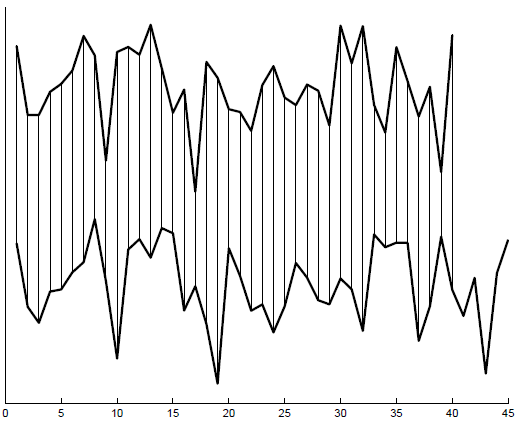
\includegraphics[width=0.5\textwidth]{./figures/euclidean_distance_time_series}
        }
        \subfloat[]{
           \label{fig:dtw_distance_time_series}
           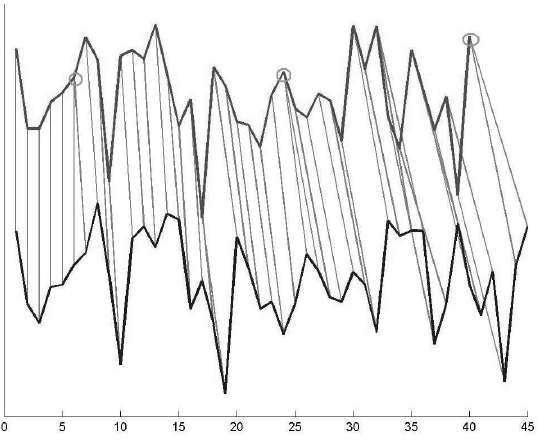
\includegraphics[width=0.5\textwidth]{./figures/dtw_distance_time_series}
        }        
    \caption{The distance between two relatively similar time series. Using the Euclidean distance as demonstrated in (a), the distance is $Minkowski_{2}(R,S)=8.68$. Using Data Time Warping as seen in (b), the distance is $DTW(R,S)=2.48$ \cite{chen2005similarity}.}
   \label{fig:time_series_distance_demo}
\end{figure}

\iftoggle{edit-mode}{\hspace{0pt}\marginpar{Next Subsections}}{}
In the following two subsections (\ref{subsec:emd} and \ref{subsec:dtw}) we will explain in details two similarity measure functions used in the thesis, the \emph{Earth mover's distance} and the \emph{Data time Warping}. 

\subsection{The Earth Mover's Distance}
\label{subsec:emd}

\iftoggle{edit-mode}{\hspace{0pt}\marginpar{Introduction to EMD}}{}
The \emph{Earth Mover's Distance} (EMD), introduced by Rubner et al. in \cite{rubner2000earth}, is a measure of the dissimilarity between histograms. It was experimentally verified to capture well the perceptual notion of a difference between images. It is commonly used in content-based image retrieval to compute distances between the color histograms of two digital images \cite{grauman2004fast}.\\

\iftoggle{edit-mode}{\hspace{0pt}\marginpar{Binwise based measures}}{}
Histogram based descriptors, such as SC, are in many cases compared using a bin-wise dissimilarity techniques such as the Minkowski distance (as defined in Equation \ref{eq:minkowski}) or the $\chi^2$ statistic as defined below.\\
 
\begin{definition}
Given two histograms $H=\{h_i\}_{i=1}^{\ell}$ and $K=\{k_i\}_{i=1}^{\ell}$ the following is defined as the $\chi^2$ statistic: 
\begin{equation}
dist_{\chi^2}(H,K)=\sum_{i}^{\ell} \frac{(h_i - m_i)^2}{m_i}
\end{equation}
where $m_i=\frac{h_i+k_i}{2}$.
\end{definition}

\iftoggle{edit-mode}{\hspace{0pt}\marginpar{Drawback of binwise based measures}}{}
Bin-wise dissimilarity measures can be computed very fast due to the fact that they measure dissimilarities between the content of corresponding bins of the two histograms and discard information across bins. However, they usually fail to consider local and global variations. These variations, which would be perceived as minor by a human, may result in a large dissimilarity values between two histograms.\\

\iftoggle{edit-mode}{\hspace{0pt}\marginpar{The transportation problem}}{}
Generally speaking, the distance between two histograms can be viewed as a special case of the well-known \emph{transportation problem}, a.k.a the Monge-Kantorovich problem \cite{rachev1985monge} defined below (Definition \ref{def:transportation_problem}). Accordingly, EMD is based on the solution to the transportation problem, for which efficient algorithms are available. \\

\begin{definition}
\label{def:transportation_problem}
Given several \emph{suppliers} and \emph{consumers}. Each supplier, $P_i$, having a given amount of goods $p_i$, and each consumer, $Q_j$, having a given amount of demand, $q_j$. For each supplier-consumer pair, the cost of transporting a single unit of goods is $d_{ij}$. The transportation problem is then to find the a least expensive flow of goods from supplier to consumer that satisfies the consumer's demand, i.e., finding the flow $f_{ij}$ between $P_i$ and $Q_j$ which minimizes:
\begin{equation}
COST(P,Q,F)=\sum_{i,j} d_{ij}f_{ij} 
\end{equation}
subject to the following constrains:
\begin{equation}
f_{ij} \geq 0, 1\leq i \leq m \wedge 1\leq j \leq n 
\end{equation}
\begin{equation}
\sum\limits_{j=1}^{n} f_{ij} \leq p_i, \forall 1\leq i \leq m
\end{equation}
\begin{equation}
\sum\limits_{i=1}^{m} f_{ij} \leq q_j, \forall 1\leq j \leq n
\end{equation}
\begin{equation}
\sum\limits_{i,j} f_{ij} = \min\left\{ \sum\limits_{j=1}^{n} q_j, \sum\limits_{i=1}^{m} p_i \right\}
\end{equation}
\end{definition}

\iftoggle{edit-mode}{\hspace{0pt}\marginpar{EMD definition}}{}
Once the general transportation problem is solved, and optimal flow $f$ was found, EMD is defined as the cost normalized by the total flow, namely the total weight of the smaller histogram. which is done in order to avoid favoring small histograms. i.e.:
\begin{equation}
EMD(P,Q)=\min\limits_{f} {\frac{\sum_{i,j} f_{ij}d_{ij}}{\sum_{i,j} f_{ij}}}
\end{equation} 

EMD is a natural and intuitive metric. Descriptively, if the histograms are interpreted as two different ways of piling up a certain amount of sand, the EMD is the minimal cost of turning one pile to other. Namely, the minimal total ground distance traveled, weighted by the amount of sand moved (called flow). When used to compare histograms with the same overall mass, namely distributions, EMD is a metric.\\

\iftoggle{edit-mode}{\hspace{0pt}\marginpar{EMD modeling as flow in graph}}{}
EMD can also be modeled as a network flow problem in graph theory. The two compared histograms are represented by a bipartite graph in which each bin is represented as a vertex and its content as the vertex value. An edge connects each bin in the left graph to every bin in the left graph. The edge's weight equals to the ground distance between the two bins. The vertices in the left side graph act as sources and the vertices in the right side as sinks. Computing EMD is now the \emph{uncapacitated minimum cost flow} problem and can be solved using Orlin's algorithm in $O(N^3 \log N)$ for N-bins histograms \cite{shirdhonkar2008approximate}.\\

\iftoggle{edit-mode}{\hspace{0pt}\marginpar{EMD in Feature space}}{}
As seen in previous sections, both CS and MAD produce histograms. The implementation used in this work for the SC produces a feature vector with a constant total mass, i.e., a distribution. In this case, EMD is a true metric, therefore, properly fit our needs.\\

\iftoggle{edit-mode}{\hspace{0pt}\marginpar{EMD in handwriting recognition}}{}
EMD was used by Saabne in \cite{saabni2013efficient} to measure similarity between shapes for recognizing and searching Arabic words. However, for the best of our knowledge, this is the first use of EMD for on-line handwriting recognition.\\

\iftoggle{edit-mode}{\hspace{0pt}\marginpar{EMD drawback}}{}
The major hurdle to using EMD is its $O\left( {{N^3}\log N} \right)$ computational complexity (for an $N$-bin histogram). The complexity is magnified when the task is to search for similar shapes (nearest neighbors) in a large database. In this case, a linear scan of the database would require computing a comparison of superpolynomial complexity for each database member against the query shape \cite{grauman2004fast}. In Section \ref{subsec:approximating_emd_using_embedding}, we will discuss an EMD embedding technique which greatly reduces the computation effort in approximating the EMD distance between two objects and also facilitates the application of indexing which spares the linear scan of the entire database.\\

\subsection{Data Time Warping}
\label{subsec:dtw}

\iftoggle{edit-mode}{\hspace{0pt}\marginpar{Introduction}}{}
\emph{Dynamic time warping} (DTW) is an algorithm for finding the optimal alignment between two time series. Intuitively, the sequences are warped in a non-linear fashion to match each other. See Figure \ref{fig:dtw_dequence_demo}. It was developed originally for speech recognition\\ 


DTW is used for solving the discrepancy between intuition and calculated distance using the alignment between the two sequences. It is done by accumulating the distance of the alignment path, i.e., summing the distance between every two corresponding points on the warping path. 

\begin{figure}[h!] 
\centering
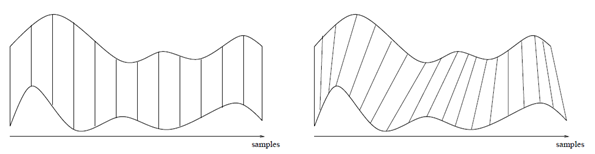
\includegraphics[width=1\textwidth]{./figures/dtw_dequence_demo}      
\caption{The right scheme shows sample-by-sample na\"{\i}ve alignment after re-sampling and in the left scheme the alignment was performed using DTW \cite{rath2003word}.}
\label{fig:dtw_dequence_demo}
\end{figure}

\iftoggle{edit-mode}{\hspace{0pt}\marginpar{Warping path Definition}}{}
\begin{definition}
Given two time series, $X = (x_1,x_2,...,x_n)$ and $Y = (y_1,y_2,...,y_m)$, the \emph{warping path} $W=(w_1,w_2,...,w_K)$ where ${w_k} = (i_k,j_k)$ is an alignment between the two sequences which satisfies the following conditions: 
\begin{enumerate}
\item Start and End point constraint: $w_1 = (1,1)$ and $w_k = (n,m)$. 
\item Local continuity constraint: ${w_{k + 1}} - {w_k} \in \left\{ {\left( {1,1} \right),\left( {1,0} \right),\left( {0,1} \right)} \right\}$
\end{enumerate}	 
The weight of a given warping path $W$ is defined as:
\begin{equation}
G(W) = \sum\limits_{k = 1}^{K} d(x_{i_k},y_{j_k} )
\end{equation}
where $d(x_{i_k},y_{j_k})$ is the distance between the points $x_{i_k}$ and $y_{j_k}$.
\end{definition}

\iftoggle{edit-mode}{\hspace{0pt}\marginpar{DTW Definition}}{}
Equipped with the definition of a warping path, DTW is defined as follows:
\begin{equation}
DTW(X,Y)=\min\limits_{W} {G(W)}
\end{equation}
Namely, DTW returns the weight of the path which is associated with the optimal alignment.\\

\iftoggle{edit-mode}{\hspace{0pt}\marginpar{Accumulated distance matrix}}{}
Using a dynamic programing approach, DTW yields the optimal warping path by constructing the \emph{accumulated distance matrix} $D \in \mathbb{R}^{m \times n}$. 
$D(i,j)$ is the minimum distance warping path that can be constructed from the two time series $X = \left( {{x_1},{x_2},...,{x_i}} \right)$ and $Y = \left( {{y_1},{y_2},...,{y_j}} \right)$. \\

The accumulated distance matrix is calculated as follows: 
\begin{algorithm}
$D(1,1) = 0$\;
\For{$i\leftarrow 2$ \KwTo $n$}{
	$D(i,1) = d(x_i,y_1)$\;
}
\For{$i\leftarrow 2$ \KwTo $m$}{
	$D(1,j) = d(x_1,y_j)$\;
}
\For{$i\leftarrow 2$ \KwTo $n$}{
	\For{$j\leftarrow 2$ \KwTo $m$}{
		$D(i,j) = d(x_i,y_j) + \min {\left\{D(i,j - 1),D(i - 1,j),D(i - 1,j - 1)\right\}}$\;
	}
}
\caption{Accumulated distance matrix ($D$) construction}
\label{alg:adm_dtw}
\end{algorithm}


Therefore, the value in $D(m,n)$ contains the minimum-distance warping path between $X$ and $Y$.
The optimal warping path $W$ is retrieved by backtracking the matrix $D$ from the point $D(m,n)$ to the point $D(1,1)$ following the greedy strategy of looking for the direction from which the current distance is taken \cite{senin2008dynamic}.\\

\iftoggle{edit-mode}{\hspace{0pt}\marginpar{stroke trajectories similarity measure using DTW}}{}
Handwritten strokes can be seen as temporal sequences in the planar space. In the on-line handwriting recognition, the exact temporal information is discarded in most cases by re-sampling the strokes to obtain equidistant sampling. However, unlike off-line handwriting recognition, the ordering information of the samples is kept. As such, DTW is an intuitive method for calculating the correspondence between two strokes. 
It have been proved relatively efficient and effective for shape matching of handwritten words. DTW was used in \cite{rath2003word, rath2003indexing, moghaddam2009application} to calculate the similarity between handwritten script in historical documents. Saabne has used DTW for key-word searching in \cite{saabni2011fast, saabni2008keyword}. \\

\iftoggle{edit-mode}{\hspace{0pt}\marginpar{DTW Speedup}}{}
One drawback of DTW is its quadratic time and space complexity, i.e., $O(mn)$ where $m$ and $n$ are the time series lengths. Therefore, several speedup methods have evolved. These methods fall into the following categories:
\begin{enumerate}
\item Constraints Enforcing: Limiting the amount of calculated cells in the accumulated distance matrix.
\item Data Abstraction: Running the DTW algorithm on an abstract representation of the data.
\item Pruning: Reducing the times DTW needs to run when determining similarity of time series.
\end{enumerate}

\paragraph{Constraints Enforcing:} 
In some cases DTW tends to create an unrealistic correspondence between time-series features by aligning short features from one of the series to the long features on the second time series. To avoid this undesired phenomenon, constrains can be imposed on the possible correspondence between several consecutive points on the warping path. Two such constraints are the Sakoe-Chuba Band \cite{sakoe1978dynamic} and he Itakura parallelogram \cite{itakura1975minimum} (Figure \ref{fig:dtw_dequence_demo}). The grayed out area is the cells of the $D$ matrix that are filled by the DTW algorithm for each constraint. The warping path is looked for in the constraint window. The width of the window is specified by a parameter. Note that such constrains limit the amount of calculation needed for computing DTW, however, the speedup factor is a constant and the DTW complexity remains quadratic. Furthermore, if the warping path is does not reside in the constraint window, it will not be found by DTW, thus, such method is usually used when the warping path is expected to be in the constrain window.

\begin{figure}
\centering
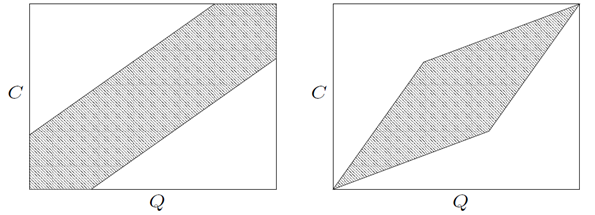
\includegraphics[width=0.7\textwidth]{./figures/dtw_sukoe_chuba}       
\caption{Cost matrix constraints: Sakoe-Chiba band (left) and the Itakura parallelogram (right).}
\label{fig:dtw_sukoe_chuba}
\end{figure}

\paragraph{Data Abstraction:} Speedup using data abstraction is performed by running DTW on a reduced presentation of the data thus reducing the cell numbers that need to be computed. The warp path is calculated on the reduced resolution matrix and mapped back to the original (full) cost matrix. \emph{FastDTW} which was proposed in \cite{salvador2007toward} is an example of such approach. 
 
\paragraph{Pruning:} Searching the most similar time series in the database given a template time series can be done more efficiently using lower bound functions than using DTW to compare the template to every series in the database. A lower-bounding is cheap and approximate. However, it underestimates the actual cost determined by DTW. It is used to avoid comparing series by DTW when the lower-bounding estimate indicates that the time series is worse match than the current best match \cite{rath2003word} (lower bounding benefits will be discussed in more details in Section \ref{subsec:lower_bounding_indexing}).\\

\iftoggle{edit-mode}{\hspace{0pt}\marginpar{How DTW is used in this work?}}{}
In this work, DTW is used for candidates scoring (described in chapter \ref{sec:candidates_scoring}) rather than similar samples spotting. Actually, nearest neighbors are found among the entire dataset based on the EMD metric. Next, DTW is employed for measuring the similarity between the test sample and its nearest neighbors


%%%%%%%%%%%%%%%%%%%%%%%%%%%%%%%%%%%%%%%%%%%%%%%%%%%%%%%
\newpage{}
%%%%%%%%%%%%%%%%%%%%%%%%%%%%%%%%%%%%%%%%%%%%%%%%%%%%%%%

\section{Similarity Search}
\label{sec:similarity_search}
 
\iftoggle{edit-mode}{\hspace{0pt}\marginpar{Introduction}}{}
In Section \ref{sec:similarity_measures}, we have discussed one aspect of information retrieval - the effectiveness of measuring the perceptual notion of similarity between two objects. However, even the most qualitative similarity measure technique is almost useless if for a given query object, the task of searching for similar objects in the database cannot be done efficiently. Efficient similarity search usually requires the development of search methods that minimize the overall search costs.\\

\iftoggle{edit-mode}{\hspace{0pt}\marginpar{Similarity search query types}}{}
Similarity based search introduce two fundamental query types: \emph{range queries} and \emph{k-nearest neighbor queries} \cite{hetland2009basic}. Formal definitions of both query types are provided in Definitions \ref{def:range_query} and \ref{def:knn_query} and visualized in Figure \ref{fig:similarity_query_types}.\\

\begin{definition}
Given a data space $D$, a distance function, $dist$, defined on $D$, a query object $q$ and a range parameter $r \geq 0$. The \textbf{range query} returns all the data objects in $D$ that are within distance $r$ from the query object $q$. Namely,
\begin{equation}
Range(q,r,D,dist)=\{o \in D | dist(q,o) \leq r \}
\end{equation}
\label{def:range_query} 
\end{definition}

\begin{definition}
Given a data space $D$, a distance function, $dist$, defined on $D$, a query object $q$ and a range parameter $r \geq 0$. The \textbf{k-nearest neighbors} (k-NN) query returns the $k$-closest objects in $D$ to the query object $q$. Namely,
\begin{equation}
k-NN(q,D,dist)=\{A \subseteq D | \forall a \in A, b \in D \setminus A: dist(q,a) \leq dist(q,b) \wedge |A|=k \}
\end{equation}
\label{def:knn_query} 
\end{definition}

\begin{figure}[h!]
	\centering
        \subfloat[]{
            \label{fig:range_query}
            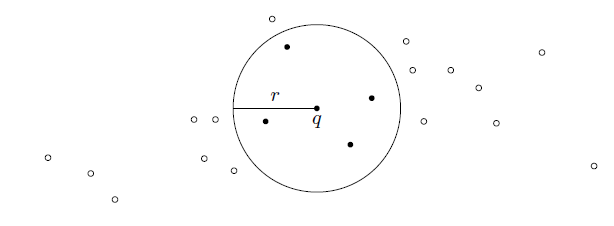
\includegraphics[width=0.5\textwidth]{./figures/range_query}
        }
        \subfloat[]{
           \label{fig:knn_query}
           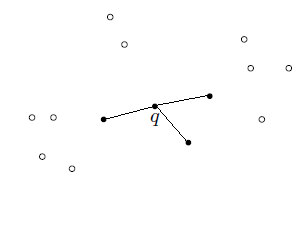
\includegraphics[width=0.5\textwidth]{./figures/knn_query}
        }        
    \caption{Visualization of the \textbf{range} (\ref{fig:range_query}) and the \textbf{$k$-NN} (\ref{fig:knn_query}) queries in the two-dimensional Euclidean space.}
   \label{fig:similarity_query_types}
\end{figure}
While range queries are argued to be fundamental, $k$-NN queries notably take a large volume in the literature. In the following we focus on $k$-NN queries.\\

\iftoggle{edit-mode}{\hspace{0pt}\marginpar{Problems - similarity search costs}}{}
The efficiency of a search method is defined as the time needed to evaluate a query. The the query efficiency is affected mainly by two components; the computation time cost and the disk access time cost. The computation cost represents the effort spent by the similarity measure function. As discussed in Section \ref{sec:similarity_measures}, effective similarity measure methods that reasonably correspond to the human intuition are costly. The I/O cost is determined by the volume of data needed to be investigated to evaluate a query. Namely, the number of samples in the dataset that needs to be examined \cite{saabni2013efficient}.\\

\iftoggle{edit-mode}{\hspace{0pt}\marginpar{Solution directions}}{}
Decreasing the computational cost can be obtained by using a cheap distance measure function which approximates, usually by providing a lower bound, the similarity between two given sample objects. The lower bound is used to filter out candidates with a similarity distance larger than a preset threshold. However, reducing the disk access cost can be attained by discarding entire portions of the dataset which are assured to be distant enough from the given query object. Such techniques are called \emph{Metric Indexing} and will be discussed in Section \ref{subsec:metric_embedding}. \\


\subsection{Lower Bounding}
\label{subsec:lower_bounding}
\iftoggle{edit-mode}{\hspace{0pt}\marginpar{Distance function approximation}}{}
In order to improve upon evaluating the distance function on every object in the dataset, we must somehow infer that an object $x$ can be included in, or excluded from, the search result without calculating the distance function $dist(q, x)$. One option to do so is by finding a cheap way of approximating the distance. Although, both lower and upper bounding measures can be exploited to avoid running expensive calculation of the distance function $dist$, lower bounding appears to be more useful, since it can be safely used to exclude far candidates as described in Algorithm \ref{alg:lower_bound}. The more the approximation function $d$ is accurate, the less the actual distance function $dist$ will be invoked. However, there will normally be a trade-off between the approximation quality and the cost of computation \cite{hetland2009basic, keogh2005exact}.\\

\begin{algorithm}
$best\_so\_far = \infty$\;
\For{every object $x$ in database}{
	\If{$d(q,x) < best\_so\_far$}{
		$dist = d(q,x)$\;
	}
	\If{$dist < best\_so\_far$}{
		$best\_so\_far = dist$\;
		$nearest\_neighbor = x$\;
	}
}
\caption{An routine that uses a lower bounding distance function, $d$, to speedup the search for the nearest neighbor of the query object q in the database under the distance function $dist$.}
\label{alg:lower_bound}
\end{algorithm}

\subsection{Metric Embedding}
\label{subsec:metric_embedding}

\iftoggle{edit-mode}{\hspace{0pt}\marginpar{A different approach}}{}
The speedup obtained by lower bounding is limited. An alternative approach is to embed the distance space imposed by the costly similarity measure, into a metric space equipped with a simple-to-compute distance function. Consequently, the calculation of distances between two elements in the embedded space would provide an inexpensive approximation to the actual distance between the two objects in the original space. A formal definition of the embedding is given in Definition \ref{def:embedding}.\\

\begin{definition}
Given metric spaces $(D, d)$ and $(D', d')$ a map $f : D \rightarrow D'$ is called an \textbf{embedding}.
\label{def:embedding}
\end{definition}

\iftoggle{edit-mode}{\hspace{0pt}\marginpar{Isometric embedding}}{}
The special case where $d(x, y) = d'(f(x), f(y))$ for all $x, y \in D$ is called \textbf{distance-preserving} or \textbf{isometric} embedding. However, isometric embeddings are very rarely beneficial. In many cases, we allow the mapping to alter the distances in a restricted manner. The distortion of the embedding is defined in Definition \ref{def:embedding_distortion}.\\

\begin{definition}
Given two metrics $(D, d)$ and $(D',d')$ and a map $f : D \rightarrow D'$, the \textbf{contraction} of $f$ is the maximum factor by which distances are shrunk, i.e.,
\begin{equation}
\max_{x,y \in D} \frac{d(x,y)}{d'(f(x),f(y))}
\end{equation}

The \textbf{expansion} of $f$ is the maximum factor by which distances are stretched. Formally:
\begin{equation}
\max_{x,y \in D} \frac{d'(f(x),f(y))}{d(x,y)}
\end{equation}

and the \textbf{distortion} of $f$ is the product of the distortion and the expansion.\\
\label{def:embedding_distortion}
\end{definition}

\iftoggle{edit-mode}{\hspace{0pt}\marginpar{$L_p$ advantage and drawbacks}}{}
Using normed spaces (see Definitions \ref{def:norm}) such as the $L_p$ norm (see Definitions \ref{lp}) to solve the dissimilarity measure problem enables using data structures that facilitate sub-linear $k$-NN retrieval, such as k-d trees. \\

\begin{definition}
Given a data space $D$, for any two data elements  $x,y \in D$, a \textbf{norm} $\|\cdot\|$ is defined as:
\begin{equation}
\|\cdot\|: D \longrightarrow \mathbb{R}
\end{equation}
where the following conditions hold:
\begin{itemize}
\item $\|x\|=0 \Leftrightarrow x=0$
\item $\|x-y\| \geq|\|x\|-\|y\||$
\item $\|\alpha x\|=|\alpha|\|x\|$
\end{itemize}
the pair $\left(D,\|\cdot\|\right)$ is called a \textbf{normed space}.
\label{def:norm}
\end{definition}


\begin{definition}
Given an vector space $V=\mathbb{R}^N$ and $v=(v_1,v_2,...,v_N) \in V$, the $L_p$ norm is defined as:
\begin{equation}
\|v\|_p=\sqrt[p]{\sum\limits_{i=1}^N v_i^p}
\end{equation}
\label{lp}
\end{definition}
In this case we will denote this vector space as $L_p^N$ to emphasize the fact is has $N$ dimensions.\\

\subsection{Approximating EMD using Embedding}
\label{subsec:approximating_emd_using_embedding}

\iftoggle{edit-mode}{\hspace{0pt}\marginpar{Indyk and Thaper Embedding}}{}
Several approximation algorithms have been proposed to speedup the computation of EMD. 
Indyk and Thaper \cite{indyk2003fast} proposed a technique for embedding the un-normed EMD metric into the $L_1$ space so that the EMD distance between the two objects is comparable to the Manhattan distance between the two points which represent the embedding of the two objects.  
Given two points sets $A$ and $B$, both of cardinality $N$ and containing points in $L_2^d$ space, the embedding given in \cite{indyk2003fast} is into the $L_1^d$ norm (i.e., the space of vectors in $\mathbb{R}^d$ equipped with the Manhattan norm) and can be described by the following: 
The general idea of the embedding is to compute and concatenate several weighted histograms of decreasing resolution for a given point set. Let us assume that the smallest distance between any two points is $1$ and $\Delta$ is the diameter of $C=A \bigcup B$, the embedding can be described as imposing hierarchy of grids $G_i$ having side length $2^i$ on the space $\mathbb{R}^d$, where $-1 \leq i \leq \log \Delta$. It is required that each grid $G_{i}$ be a refinement of the grid $G_{i+1}$. 
Each grid is translated by a vector chosen randomly from $[0, \Delta]^d$. For each grid $G_i$, the vector $v_i(A)$ contains a single coordinate per cell that contains the number of points in the corresponding cell. In fact, for every $i$, $v_i(A)$ forms a histogram of A. The embedding, denoted as $f_{EMD}(A)$, is then defined as the concatenated vector of the $v_i$'s, scaled by the grid side lengths. Formally,
\begin{equation}
f_{EMD}(A) = [v_{-1}(A)/2, v_0(A), 2v_1(A), 4v_2(A),..., 2^iv_i(A),...]
\end{equation} 
Figure \ref{[]} provides a visual demonstration of the embedding.\\

Approximating the EMD distance between the set $A$ and $B$ is then done by calculating the Manhattan distance between the two corresponding embedding vectors, i.e.,
\begin{equation}
EMD_{approx.}=|f_{EMD}(A) - f_{EMD}(B)|
\end{equation}  

\iftoggle{edit-mode}{\hspace{0pt}\marginpar{Performance}}{} 
The time complexity of the embedding is $O(Nd \log{\Delta})$. The distortion of the embedding has an upper bound of $O(\log \Delta)$. A detailed proof is provided in \cite{indyk2003fast}. However, the proved theoretical distortion can only provide a weak practical instrument. Nevertheless, experimental validation performed on a dataset of $20,000$ objects showed a $(1+\epsilon)-approximate$ nearest neighbor, with $\epsilon < 20\%$ achieved by the embedding compared to the exact EMD in \cite{indyk2003fast}. Grauman and Darrel \cite{grauman2004fast} have used this embedding for contour matching and experimentally validated the quality of retrieval. They have found that the accuracy reduction is less than $10\%$ compared to the exact EMD.\\

\subsubsection{EMD Embedding using the wavelet Coefficients Domain}
%How it is done?
%Is it faster to calculate?
%Is the retrieval more accurate (empirically) than the $L_1-EMD$ embedding?
%Are the bounds are more strict?

\iftoggle{edit-mode}{\hspace{0pt}\marginpar{Wavelet embedding}}{}
In a subsequent work done by Shirdhonkar and Jacobs \cite{shirdhonkar2008approximate}, the authors proposed a method for approximating the EMD between two low dimensional histograms using the weighted wavelet coefficients of the difference histogram. The approximation is done by transforming the histograms into the $L_1$ space so that the distance between the two vectors in the wavelet domain is the EMD approximation. They proved the ratio of EMD to wavelet EMD is bounded by constants. In the following, a background on wavelets is required and the user is referred to Appendix A for a brief introduction on the subject.\\

\iftoggle{edit-mode}{\hspace{0pt}\marginpar{EMD embedding to the wavelet domain}}{}
Shirdhonkar and Jacobs showed that the embedding of the difference histogram approximates the EMD between two histograms. It is done by calculating the $L_1$ norm of the coefficients vector of the embedding as given in Equation \ref{eq:emd_embedding}.
\begin{equation}
d(p)_{wemd}= \sum\limits_{\lambda} 2^{-j(1+n/2)}|p_{\lambda}|
\label{eq:emd_embedding}
\end{equation}
where $p$ is the n-dimensional difference histogram and $p_{\lambda}$ is the wavelet transform coefficients. The index $\lambda$ includes both shifts and the scale j.\\

\iftoggle{edit-mode}{\hspace{0pt}\marginpar{Intuitive explanation}}{}
Intuitively, the wavelet transform splits up the difference histogram according to scale and location where each coefficient represents the solution to the EMD subproblem. For a single wavelet, the mass to be moved is proportional to the volume of $|\psi_j(x)|$, i.e., to $2^{-jn/2}$ and the distance to be traveled is proportional to the span of the wavelet, i.e $2^{-j}$. The sum of all distances is an approximation to EMD, as formally defined in Equation \ref{eq:emd_embedding}. 
This can be viewed as similar to the way packages are shipped over large distances. The route is broken into several pieces which are large and small distances. Packages from nearby places are merged at the end of the short distance route piece to travel together. Then another merge is done of packages from the entire country to be shipped together to the destination country. The sum of the distances traveled is an approximation to the actual distance. See Figure \ref{fig:emd_wavelet}.\\

\begin{figure}
\centering
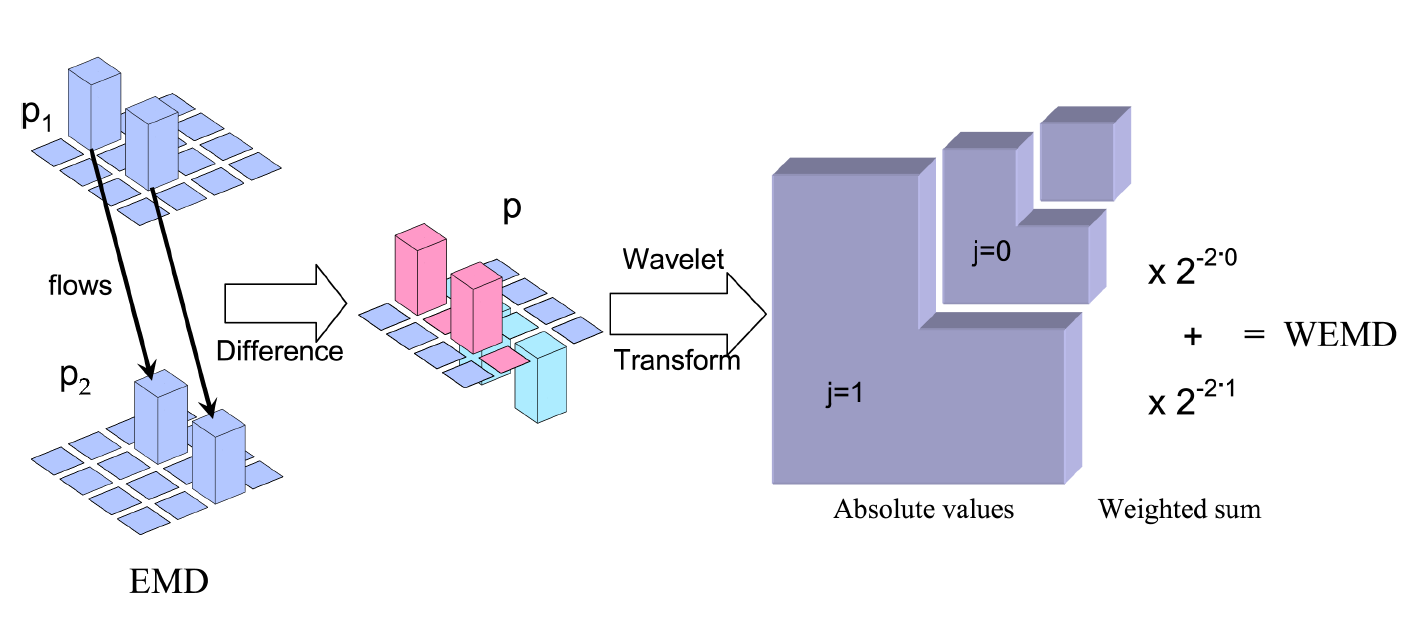
\includegraphics[width=1\textwidth]{./figures/emd_wavelet}       
\caption{EMD embedding using the wavelet domain \cite{shirdhonkar2008approximate}.}
\label{fig:emd_wavelet} 
\end{figure}

\iftoggle{edit-mode}{\hspace{0pt}\marginpar{Embedding the histograms rather than the difference histogram}}{}
However, in our application, where the histogram descriptors are to be stored rather than the difference histogram, the computation of EMD can be partitioned into two parts. First the histograms are converted into the wavelet domain and their coefficients are scaled according to Equation \ref{eq:emd_embedding}. 
Computing the EMD distance, in the next step, is done by calculating the Manhattan distance between the scaled coefficients of the corresponding histograms.\\

\iftoggle{edit-mode}{\hspace{0pt}\marginpar{shirdhonkar - theoretical and empirical bounds}}{}
They provided both theoretical and experimental bounds. The theoretical approximation is based on Theorem 2 in \cite{shirdhonkar2008approximate}. Using a large dataset, they were able to experimentally establish that the proposed approximation follows the true EMD closely empirically and can be alternatively used without any significant difference in performance. The wavelet EMD metric can be computed in $O\left( N \right)$ time complexity. The authors tested few wavelets and showed that the Coif-lets of order 3 and the Symmetric Daubechies wavelets of order 5 have lowest error rates. We followed their results and have chosen to work with the order 3 Coif-lets.\\

\iftoggle{edit-mode}{\hspace{0pt}\marginpar{Performance - Indyk vs. shirdhonkar}}{}
Empirically, the normalized RMS error obtained by using the wavelet embedding was between in 13\% and 20\% compared to the embedding proposed by Indyk and Thaper which achieved 43\% in the same experiment. In addition, the wavelet embedding surpassed the Indyk and Thaper embedding in time performance. Note that the embedding process requires histograms, thus the vectors in the feature space need to be normalized before using this method.

\subsection{Metric Indexing}
\label{subsec:metric_indexing}

\iftoggle{edit-mode}{\hspace{0pt}\marginpar{Motivation}}{}
Distance function approximation techniques alone cannot avoid linear scan of the entire dataset when searching for the nearest neighbors of a query object. In order to speedup queries, index structures should be build over the dataset. The main goal of an index method is to enable efficient search, either asymptotically or simply in real wall-clock time. The time cost involved in building the index is amortized over the series of queries, and is usually ignored when considering search cost \cite{hetland2009basic}.\\

\iftoggle{edit-mode}{\hspace{0pt}\marginpar{Introduction}}{}
Efficient data retrieval in a metric dataset requires building a \emph{metric index}. Indexing techniques partition the dataset into equivalent classes such that each equivalent class contains objects that are sufficiently close to each other. However, this does not assure that close objects will always be contained in the same equivalent class. Each class is bounded by a hypersphere covering all the objects in the class. Consequently, at query time the metric index is efficiently searched to locate the equivalent classes which cover the areas where the closest objects may be contained. These classes are then exhaustively checked for the relevant objects.
This allows discarding classes that surely does not contain relevant objects. In order for the metric indexing to work correctly and efficiently, the distance function is required to satisfy the triangle equality.\\
 
\iftoggle{edit-mode}{\hspace{0pt}\marginpar{Exact vs. Approximate Indexing}}{}
Indexing techniques are split into two types: exact and approximate. Exact techniques are guaranteed to return the same result as  scanning the entire database. Approximate indexing methods return good matches but not necessarily the best matches. Exact methods do not allow false positives or false negatives, i.e., all of the relevant objects are required to be returned in the query result, and only them. However, the approximate methods relax this strong requirement so that a small number of false negatives is acceptable \cite{keogh2005exact}. Many methods were proposed to solve the $k$-NN problem that are significantly better than a brute-force computation over the entire database. However, computing nearest neighbors approximately, can achieve significantly faster retrieval with a relatively small actual errors. \emph{Approximate nearest neighbor} (ANN) techniques also allow the user to specify a maximum approximation error bound, thus enabling the user to control the trade-off between accuracy and running time. \\

\begin{figure}
\centering
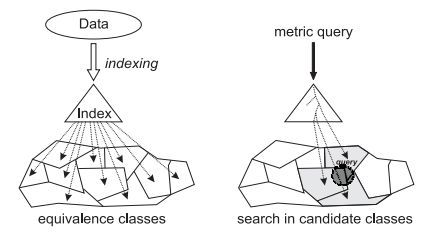
\includegraphics[width=0.7\textwidth]{./figures/indexing}       
\caption{Metric Indexing. \emph{Add citation}}
\label{fig:indexing}
\end{figure}


\iftoggle{edit-mode}{\hspace{0pt}\marginpar{Examples of Exact and Approximate Indexing}}{}
ANN methods such as k-d trees (will be described later) and Locality Sensitive Hashing (LSH) \cite{gionis1999similarity} have been successfully applied on a variety of fast similarity retrieval problems. The key assumption in these procedures is that the objects in the dataset lie in a metric space, i.e., the space satisfies the triangle equality. As mentioned in chapter \ref{sec:similarity_measures}, this assumption is not valid for many similarity measure techniques. In the case of k-d tree, it requires a more specific $L_p$ metric space for its operation. While the worst case scenario complexity is $O(N)$, the expected complexity of a single $k$-NN query using k-d tree is $O(\log N)$.\\

\iftoggle{edit-mode}{\hspace{0pt}\marginpar{This work}}{}
In our framework, sub-strokes classification is done by finding sample letters in the training set that are similar to the shape of the sub-stroke. Our feature vectors were embedded into the $L_1$ space by using the wavelet embedding technique described earlier and thus metric indexing methods can be applied. While the advantage of LSH is that it performs better than k-d tree in high dimensional spaces, k-d tree can be used both as an exact and approximate $k$-NN technique. In this work, we have chosen to work with k-d tree since we could obtain, after applying dimensionality reduction techniques, a low dimensional data space.\\

%%%%%%%%%%%%%%%%%%%%%%%%%%%%%%%%%%%%%%%%%%%%%%%%%%%%%%%
\subsubsection{k-d tree}
\label{subsubsec:kd_tree}

\iftoggle{edit-mode}{\hspace{0pt}\hspace{0pt}\marginpar{A short introduction to k-d tree}}{} 
k-d tree, a special case of binary space partitioning trees, is a data structure for storing a finite set of points from a $k$-dimensional space. It was proposed by Bentley in \cite{bentley1975multidimensional}. It aims at solving the problem of searching $k$-NN in a large set of multi-dimensional points by first building a data structure based on the set of reference points. Then, given a query object, it extracts the $k$-NN using this structure.\\

\iftoggle{edit-mode}{\hspace{0pt}\marginpar{How it works, how the data is saved and extracted}}{} 
The k-d tree is formed as follows: Every point is either a branch node or is contained in a leaf node. Every branch node in the tree is associated with one of the k-dimensions and can be though of an hyperplane that divides the space into two half spaces in that dimension. Points to the left of this hyperplane are represented by the left subtree of that node and points to the right of the hyperplane are represented by the right subtree, see Figure \ref{fig:kd_tree}. A desired property of the partition is to be as equal as possible. The selection of the pivot point (i.e,  the point that function as a branch node) in every level has a great impact on the balance of the tree. The most common way is to find the medial point of a number of points in the subtree. The number of points in a leaf node is also customizable and is mostly affected by the cardinality of the points in the database and $k$, which is a predefined in many applications.

\begin{figure}
\centering
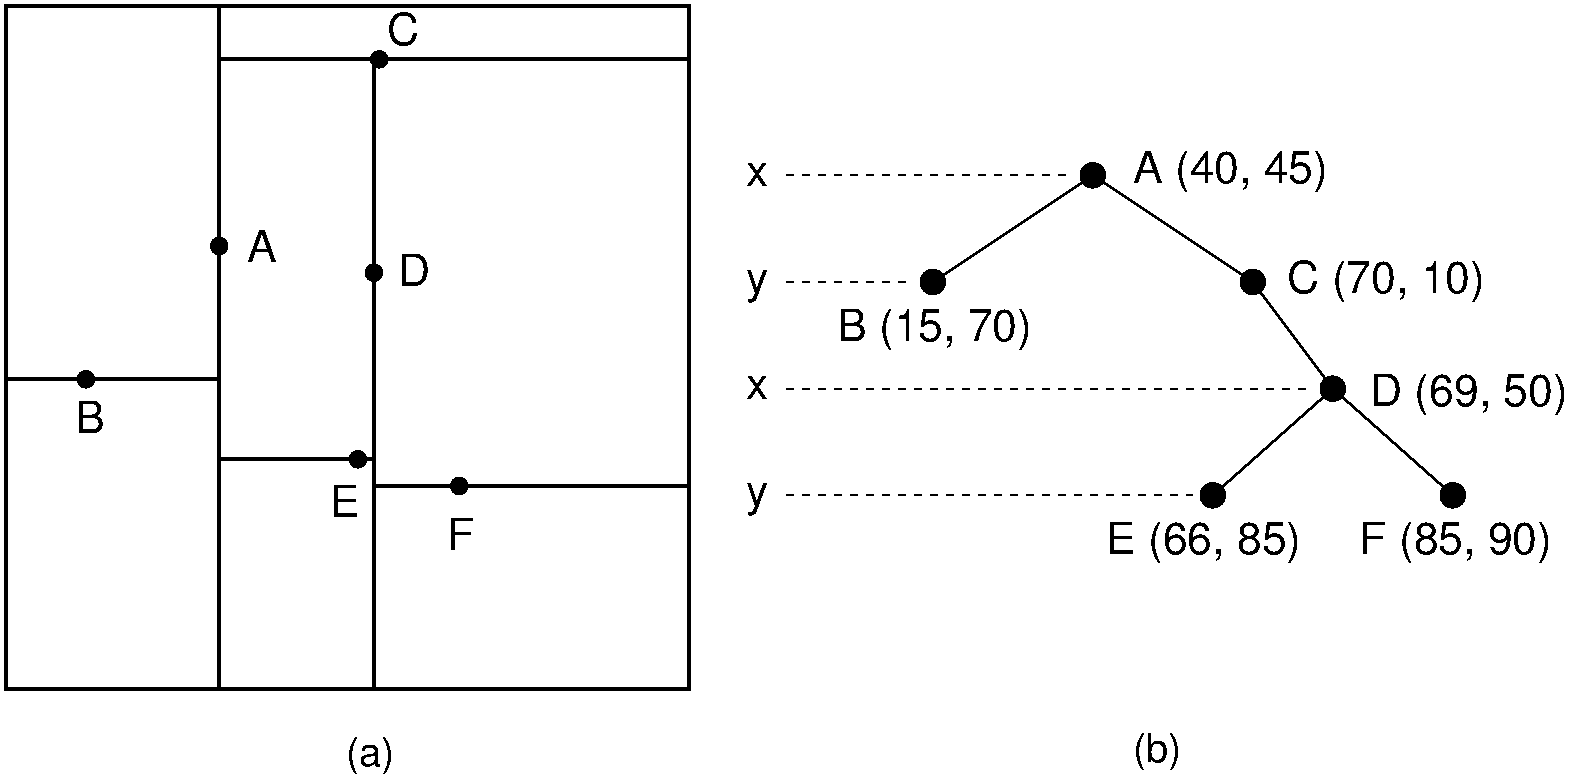
\includegraphics[width=0.8\textwidth]{./figures/kd_tree}       
\caption{Example of a k-d tree. (a) The k-d tree decomposition  a region containing seven data points. (b) The k-d tree for the region of (a).}
\label{fig:kd_tree}
\end{figure}

\iftoggle{edit-mode}{\hspace{0pt}\marginpar{How the NN are found?}}{}
The approximation of the $k$-NN using k-d tree is done by initially finding the leaf node that represents the class that the query point belongs to. Although it is probable that the $k$ nearest neighbors are all contained in a single leaf node, it is not necessarily the case. Adjacent leafs may be examined by recursively explore the other child nodes and look for near neighbors. Precise details of the algorithm can be found in \cite{bentley1975multidimensional}.\\
 
\iftoggle{edit-mode}{\hspace{0pt}\marginpar{Expected time complexity}}{}
The construction time of the k-d tree is O($k N \log N$), where $k$ is the dimensionality of the data space and $N$ is the cardinality of the dataset. We can afford this high complexity of the construction since the this process is done off-line, and theoretically will be executed mostly several times. However, this tax pays off when it comes to the enhancement we achieve in the k-$NN$ query evaluation. While the worst case scenario the running time of $k$-NN is $O(N^{d^2})$, the amortized running time is $O(\log N)$.\\

\iftoggle{edit-mode}{\hspace{0pt}\marginpar{The Matlab library}}{} 
Our system uses a built-in Matlab implementation for k-d tree which is available in the statistical toolbox and introduced in Matlab R2013B. The library allows configuring the distance function (Euclidean, Manhattan, Mankowski, etc...) and the size of the leaf node. The library provides implementation for the exact version of k-d tree.\\

%%%%%%%%%%%%%%%%%%%%%%%%%%%%%%%%%%%%%%%%%%%%%%%%%%%%%%%
\newpage{}
%%%%%%%%%%%%%%%%%%%%%%%%%%%%%%%%%%%%%%%%%%%%%%%%%%%%%%%

\section{Sample set Redistribution}
\label{sec:sample_set_redistribution}

\iftoggle{edit-mode}{\hspace{0pt}\marginpar{Motivation}}{}  
On the one hand a large and verified sample set is crucial for every learning algorithm, in particular, it is important in the handwritten pattern classification because of the variety of styles between people in their handwriting. On the other hand, a large sample set can harm the performance of the NN based recognition system, and even harm the accuracy of the recognition because of outliers. 
As can be seen in Section \ref{[]}, for some letters positions many samples were collected. And for other letters smaller set of samples were collected. On the one hand, we would like to maintain the underlying letters distribution since the distribution of our sample set has a high correlation to the real world letter distribution. On the other hand, as we have mentioned before, a non proportional sample size for some letters may harm our recognition process.\\

\iftoggle{edit-mode}{\hspace{0pt}\marginpar{Introduction}}{}
Cluster analysis is a common approach used in both supervised and unsupervised learning. It aims to partition a set of objects  into groups in such a way that objects in the same group (called a cluster) are more similar (in some sense or another) to each other than to those in other groups.
Clustering has two main uses; the first is deriving a reduced representation of the full data set. the second use is deducing new insights into the structure of the data.
Since a cluster is a notion that cannot be precisely defined, thus there is no objectively correct clustering and this is the reason there are so many clustering algorithms.
There are many clustering models. By models we mean the basic concept on which the clustering is based upon. The most prominent models are the \emph{Connectivity models}. In this group we can find the hierarchical clustering. Another widely used set of models is the \emph{Centroids models} which contain such as well known k-means algorithm. Cluster analysis is used for various goals. In non-supervised learning, when the class label are not available, this technique enable the classification system to impose classes on the sample set. In the supervised learning, it can be used to impose a hierarchy on the sample set and by doing so improving the classification performance and accuracy.\\

\iftoggle{edit-mode}{\hspace{0pt}\marginpar{What type of clustering did we use, and why. $L_1$ K-medoids}}{}
The problem of disproportional number of samples per letter class we solved by using the clustering k-medoids algorithm. the k-medoids algorithm aims to break up the dataset into k clusters. A medoid is a representative object of a cluster whose average dissimilarity to all the objects in the cluster is minimal. The k-medoids algorithm finds the k medoids of a dataset. 
k-medoids can work with an arbitrary matrix of distances between data points. In our case the distance function is $L_1$. 
Our decision to use the k-medoids algorithm rather than the common k-means algorithm is derived from obtain a digest of the dataset. Thus the returned $k$ objects by the k-medoids algorithm will function as the representatives of the samples in a given class.\\

\iftoggle{edit-mode}{\hspace{0pt}\marginpar{Short description of the k-medoids algorithm}}{}
k-medoids operates as follows: first it selects $k$ objects in random, named $M$ of the in datapoints and associate each datapoint to the closest object in $M$. Then, for each element $m$ in $M$ and for each object $o$ in the data set, swap $m$ and $o$ and compute the total cost of of the configuration, and select the configuration, with the lowest cost. Repeat the mentioned until the is no change in the set $M$. \emph{TODO: fix this flabby description.} \\ 


\iftoggle{edit-mode}{\hspace{0pt}\marginpar{When it is applied? How did we determine the number of clusters per each letter, and the number of elements in each cluster.}}{}
As mentioned before, the number of sample instances per class may greatly affect the classification result. Thus, we would like that the number of samples of each class will be distributed correspondingly to the apriory probability of the appearance of the letter in a given text. Since the letters were taken from the same database as the test set, it could have achieved optimistic results since the lexicon is the same lexicon of ~930 Tunisian cities. Thus the redistribution of letters according there apriori probability to the general Arabic text probability. We pretend to to be context free, thus this step is necessary. In addition to the fact the we have achieved very disproportion of class representative in the sample set. \\    

\iftoggle{edit-mode}{\hspace{0pt}\marginpar{How did affect our results.}}{}  
On the one hand, as claimed above, leaving the original distribution may result in a too good results since it will distributed according the letters aproiri probability appearance. On the other hand the classification results may be hurt because of outliers that affect the NN algorithm. Here we would like to show classification results of before and after samples redistribution. In the following table we show the results of the test we have conducted as follows: We have created a test set of letters and reported the percentage of the recognition rate.\\
 
%%%%%%%%%%%%%%%%%%%%%%%%%%%%%%%%%%%%%%%%%%%%%%%%%%%%%%%
\newpage{}
%%%%%%%%%%%%%%%%%%%%%%%%%%%%%%%%%%%%%%%%%%%%%%%%%%%%%%%

\section{Dimensionality Reduction}
\label{sec:dr}

\iftoggle{edit-mode}{\hspace{0pt}\marginpar{What is DR and what techniques are there?}}{}
\emph{Dimensionality Reduction} is a process of reducing the number of variables taken into consideration in the learning and classification of data. It is a very important process in machine learning since it facilitates classification, efficient storing and visualization of high-dimensional data. The undesired properties of high-dimensional data present many mathematical challenges and practical complications \cite{van2009dimensionality}. First, Analysis of high-dimensional data generally requires a large amount of memory and computation power, which may be impractical for on-line classification systems and obstructive in other applications. In particular, many NN methods such as k-d tree are ineffective when the dimensionality of the data is high.
Second, the classification algorithm is more likely to overfit the training sample and generalizes poorly to new samples \cite{aida2009word}.\\

\iftoggle{edit-mode}{\hspace{0pt}\marginpar{data Intrinsic dimensionality}}{}
Ideally, the reduced representation should have a dimensionality that corresponds to the intrinsic dimensionality of the data \cite{van2009dimensionality}.
The intrinsic dimensionality of data is the minimum number of parameters needed to account for the observed properties of the data.\\ 

\iftoggle{edit-mode}{\hspace{0pt}\marginpar{The underlying belief}}{}
The belief underlying the existence of a compact representation of the external world data is based on the observation that the human brain can instantaneously and precisely recognize an observed apple, smile or a handwritten letter within a short route of neural computations. However, a digital representations of these images may consist of hundreds or thousands of pixels. Thus, clearly, there are much more compact representations of images, sounds, and even text than their native digital formats. Many recently proposed dimensionality reduction techniques are based on the intuition that data lies on or near a complex low-dimensional manifold that is embedded in the high-dimensional space.\\

\iftoggle{edit-mode}{\hspace{0pt}\marginpar{The curse of dimensionality}}{}
The high dimensional data phenomenon is widespread in data analysis and was given the name \emph{the curse of dimensionality}. In many pattern recognition applications, the problem of high dimensional data can arise in different stages of the learning and classification process; 1. the dimensionality of the data may be high in the first place; 2. features calculated on the data may be impractically large; 3. other manipulations performed on the data, such as the embedding used in this work, may produce highly dimensional vectors. \\

\iftoggle{edit-mode}{\hspace{0pt}\marginpar{Mathematical Definition}}{}
Mathematically, given $p$-dimensional variable $x \in \mathbb{R}^p$, the dimensionality reduction process finds a lower dimensional representation $s \in \mathbb{R}^k$ with $k \leq p$ which preserves the content of the original data under a given criterion. The reduced dimensionality $p$ is chosen to be as small as possible, but yet sufficiently large to guarantee that the output vector $s$ provide a faithful representation of the input vector $x$. Dimensionality reduction techniques can be classified into linear and non-linear. Linear dimensionality reduction is based on a linear projection of the data assuming the data resides close to a lower dimensional linear subspace. Namely, each of the components in the vector $s$ is a linear combination of the components in the vector $x$, formally:
\begin{equation}
s=Wx
\end{equation}
where $W_{k \times p}$ is the linear transformation.\\

\iftoggle{edit-mode}{\hspace{0pt}\marginpar{Linear DR}}{}
\emph{Principal component analysis} (PCA) and \emph{linear discrimination analysis} (LDA) are traditional linear dimensionality reduction techniques.\\

\iftoggle{edit-mode}{\hspace{0pt}\marginpar{Non-Linear DR}}{}
In some cases, linear dimensionality reduction techniques perform poorly and a more powerful approach is required to provide the mapping from the high dimensional space to the low dimensional space. In such cases, non-linear techniques is are used. Yet, the drawback of such technique is concealed in its generality which may cause over-fitting the sample set and not really capture the true underlying coordinate system. Commonly used non-linear technique include \emph{Kernel PCA}, \emph{Isometric Feature Mapping} (ISOMAP) and \emph{Locally-linear embedding} (LLE).\\

\iftoggle{edit-mode}{\hspace{0pt}\marginpar{Why do we need DR?}}{}
The need for employing dimensionality reduction in this work emerged from the sparse vectors produces by the EMD embedding of the feature vectors into the wavelet domain procedure which was described in Section \ref{subsec:approximating_emd_using_embedding}. This process produced vectors in $R^{3946}$. The wish to employ k-d trees, which is very sensitive to high dimensional data, was the main reason for using dimensionality reduction. An alternative was to use a $k$-NN data-structure that performs well with high dimensional data such as LSH \cite{gionis1999similarity}. However, it would be less accurate since LSH is an approximate NN search method, unlike k-d tree which finds the exact $k$-NN samples.\\

\iftoggle{edit-mode}{\hspace{0pt}\marginpar{What DR we use?}}{}
In this thesis we have chosen to work only with linear dimensionality reduction techniques. PCA and LDA were applied sequentially in order to obtain linearly discriminative information in an efficient manner.\\

\iftoggle{edit-mode}{\hspace{0pt}\marginpar{PCA}}{}
\emph{Principle Component Analysis} (PCA) was invented in 1901 by Karl Pearson. Although there are many linear dimensionality reduction techniques, PCA is by far the most popular. PCA is unsupervised in the sense that the labeling of the data do not effect the determination of the transformation function. It produces an orthogonal linear transformation that transforms the data to a new coordinate system such that the greatest variance by any projection of the data comes to lie on the first coordinate (the first principal component), the second greatest variance on the second coordinate, and so on (as seen in Figure \ref{fig:pca_demo}). The principal components as a whole form an orthogonal basis for the space of the projected data. Given a multivariate dataset visualized as a set of coordinates in a high-dimensional data space, PCA obtains the "shadow" of that dataset when viewed from its most informative viewpoints by projecting the dataset into a lower-dimensional space. This is done by using only the first few principal components.\\

\begin{figure}
\centering
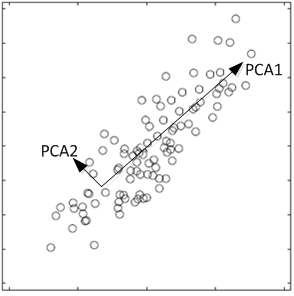
\includegraphics[width=0.5\textwidth]{./figures/pca_demo}       
\caption{The first and second principal component, PCA1 and PCA2 respectively.}
\label{fig:pca_demo}
\end{figure}

\iftoggle{edit-mode}{\hspace{0pt}\marginpar{PCA formulation}}{}
In computational terms the principal components are found by calculating the eigenvectors and eigenvalues of the data covariance matrix. This process is equivalent to finding the axis system in which the co-variance matrix is diagonal. The eigenvector with the largest eigenvalue is the direction of greatest variation, the one with the second largest eigenvalue is the (orthogonal) direction with the next highest variation and so on. The eigenvalues represent the distribution of the source data's energy among each of the eigenvectors, where the eigenvectors form a basis for the data. The representation content $g$ for the $j^{th}$ eigenvector is the sum of the energy content across all of the eigenvalues $\lambda_k$ from 1 through $j$ :
\begin{equation}
g[j]=\sum_{k=1}^{j}\lambda_k \text{   for   } j=1,...,d,
\end{equation}
where $d$ denotes the dimensionality of the original data. The \emph{data preservation rate} value (E) is calculates as seen in Equation \ref{eq:dr_energy}. 

\begin{equation}
E[L] = \frac{g[L]}{g[d]}
\label{eq:dr_energy} 
\end{equation} 

The goal is to find the smallest possible value of $L$ that achieves $E[L]$ value which rise above a preset threshold $e$, usually larger than 0.9. This approach is a well-known dimensionality estimation technique known as the \emph{eigenvalue-based dimensionality estimator}. It is a member of the \emph{global dimensionality estimator} family. Later on in this section we will mention other type of dimensionality estimator family named \emph{local dimensionality estimator}.\\

\iftoggle{edit-mode}{\hspace{0pt}\marginpar{LDA}}{}
The major drawback of PCA is that it is an unsupervised technique and as such does not use label information of the data. The following example, given by Welling in \cite{welling2005fisher}, demonstrates the problem in using PCA: in Figure \ref{fig:cigarettes_data}, we see two cigar like clusters. The samples in the upper cigar are classified as $y=1$ and the samples in the other cigar are classified as $y=-1$. The cigars are parallel and very close to each other. The variance of the entire sample set, disregarding the labels, is in the direction of the cigars. Projecting the sample set on the principal component, in this case, would be terribly mix the samples. Clearly, a better projection would be orthogonal to the cigars, namely in the direction of least overall variance, which would perfectly separate the two classes.
LDA, a descendant of the original Fisher-LDA that was proposed by Fisher in \cite{fisher1936use}, overcomes this problem. Unlike PCA, LDA is a supervised technique, i.e., it explicitly attempts to model the difference between classes of data based on the samples labeling. In this method, variability among the feature vectors of the same class is minimized and the variability among the feature vectors of different classes is maximized. LDA performs dimensionality reduction while preserving as much of the class discriminatory information as possible. A brief tutorial on LDA is given in \cite{balakrishnama1998linear}. Without going into the math, in order to find a good projection vector, we need to define a measure of separation between the projections. The solution proposed by Fisher is to maximize a function that represents the difference between the means, normalized by a measure of the within-class scatter. LDA has three main drawbacks; the first is that it assumes that the data resides in $L_2$; second, LDA assumes that the distribution of the samples in each class is Gaussian which is not necessarily true for our samples; third, it is much slower to calculate compared to PCA.\\

\emph{TODO: LDA demo image.}\\

\begin{figure}
\centering
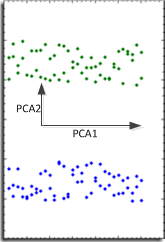
\includegraphics[width=0.3\textwidth]{./figures/cigarettes_data}       
\caption{A cigarettes like samples data spread. In this case PCA performs badly.}
\label{fig:cigarettes_data}
\end{figure}

\iftoggle{edit-mode}{\hspace{0pt}\marginpar{Why do we use both LDA and PCA?}}{}
Even though LDA is preferred in many application, it does not always outperform PCA. In order to optimize discrimination performance in a more generative way, a hybrid dimension reduction model combining PCA and LDA is used in this work.\\

\iftoggle{edit-mode}{\hspace{0pt}\marginpar{When to perform the DR?}}{}
Grauman et al. in \cite{grauman2004fast} used PCA to find a low-dimensional subspace based on a large sample of the shape context histogram. PCA yields the set of bases that define a low-dimensional "shape context manifold". Only then the approximate EMD embedding is performed. However, we have chosen to perform the stages in a different order. First, approximate EMD embedding is performed on the feature vectors, and only then, dimensionality reduction procedure is applied to reduce the dimensionality of the sparse embedded vectors. The reason we have chosen to perform the stages in this order is that if we were to apply the order suggested by Grauman, we would still result in a large sparse vectors constructed by the embedding process.\\
  
\iftoggle{edit-mode}{\hspace{0pt}\marginpar{Usage of PCA in the $L_1$ space.}}{}
The basic form of PCA is defined over the $L_2$ space. However, the data that is embedded to the wavelet domain was proved to approximate EMD in the $L_1$ space. Although $L_1$-PCA techniques were examined in the literature \cite{kwak2008principal}, we decided to use the basic form of PCA, given that $L_2$ estimate $L_1$ fairly well.\\

\iftoggle{edit-mode}{\hspace{0pt}\marginpar{Implementation: PCA}}{}
In the proposed system, we wanted to exploit the strengthens of both PCA and LDA techniques using the dimensionality reduction process which is outlined as follows: The samples are projected to a subspace $S_1$ using PCA and then to subspace $S_2$ using LDA. In the PCA stage, the target dimensionality, i.e., the number of principal components taken into consideration, is the minimal to achieve data preservation rate of 99\%, i.e., $E=0.99$. As mentioned before, the dimensionality of the original vectors was 3946. The reason we adopted such a high rate is that it was enough to achieve a very major dimensionality reduction. As seen in table \ref{table:dr_dimensions_results}, the dimensionality was reduced by PCA in two orders of magnitude. \\

\iftoggle{edit-mode}{\hspace{0pt}\marginpar{Implementation: Clustering and LDA}}{}
Applying LDA directly on the resulted data would have achieved poorer results for the reason that almost all letters in the Arabic writing system have several shapes which are commonly used. See Figure \ref{table:letters_writing_styles}. Furthermore, since LDA regards the labeling of the data samples, trying to group different perceptual shapes in a single class would impinge the dimensionality reduction process. 
In order to overcome this obstacle, we have done the following preprocessing steps: each class, namely the tuple $(letter, position)$, was clustered into four clusters using $L_1$-k-medoids algorithm. Each cluster received a different class label. This new artificially labeled data was given as input to LDA.\\

\begin{table}
\centering
\begin{tabular}{ | c | c | c | c |}
\hline
English  & Form 1 & Form 2 & Form 3\\
\hline                 
  A(Iso) &  &  &  \\ 
  \hline
  H(Fin) &  & & \\ 
  \hline
  H(Mid) &  & &  \\ 
  \hline
  NY(Fin) &  &  & \\ 
  \hline
  LM & &  &  \\ 
  \hline
  7(Mid) & & & \\ 
  \hline
\end{tabular}
\caption{Arabic Letters writing styles.}
\label{table:letters_writing_styles} 
\end{table}

\iftoggle{edit-mode}{\hspace{0pt}\marginpar{LDA target dimensionality}}{}
As aforementioned, the target number of dimensions of the PCA step were determined according to the data preservation rate parameter which was preset to $E=0.99$. This, as shown before, can be calculated easily using the eigenvalues of the covariance matrix. However, in the LDA step we have adopted a different approach to determine the target number of dimensions. \emph{Intrinsic dimensionality estimation} methods are traditional techniques for estimating the intrinsic dimensionality of a data. While there are many techniques, many use the same basic concept. They are based on the observation that for a given data point $x_i$, the number of sample points covered by a hypersphere around the data point with radius $r$ grows proportional to $r^d$, where $d$ is the intrinsic dimensionality of the data manifold around that data sample.  
The function that estimates this relation for a given data point $x_i$ is named \emph{local estimator}.
The estimated intrinsic dimensionality $\hat{d}$ of the dataset is then calculated by averaging over the local estimators of the entire sample set \cite{van2007introduction}.\\

\begin{table}
\centering
\begin{tabular}{ | c | c | c | c |}
\hline
Letter position & Number of samples & PCA & PCA+LDA\\
\hline                 
  Iso & 1372 & 29 & 7 \\ 
  \hline
  Ini & 1405 & 39 & 9 \\ 
  \hline
  Mid & 1196 & 36 & 8 \\ 
  \hline
  Fin & 1629 & 27 & 7 \\ 
  \hline
\end{tabular}
\caption{The dimensionality of the data samples is shown for every database. The original data set dimensionality is 3946. The PCA column shows dimensionality of the data after applying PCA. The PCA+LDA column shows the dimensionality of the data after applying LDA subsequently after LDA as described.}
\label{table:dr_dimensions_results} 
\end{table}

\iftoggle{edit-mode}{\hspace{0pt}\marginpar{The DR package}}{}
\emph{Matlab Toolbox for Dimensionality Reduction} described in \cite{van2007introduction} was used as Matlab wrapper for the dimensionality reduction techniques used in this work.

%%%%%%%%%%%%%%%%%%%%%%%%%%%%%%%%%%%%%%%%%%%%%%%%%%%%%%%
\newpage{}
%%%%%%%%%%%%%%%%%%%%%%%%%%%%%%%%%%%%%%%%%%%%%%%%%%%%%%%


\section{Letters Classification and Candidates Scoring}
\label{sec:candidates_scoring}

\iftoggle{edit-mode}{\hspace{0pt}\marginpar{Introduction}}{}
After discussing in details the theory underline each stage of the recognition process, in this sub section we will provide a high level description of the system and show how all the elements integrate together to build the recognizer. Also, we will drill down to describe the parameters used in every stage that were tunned to obtain the achieve the best results.\\ 

\iftoggle{edit-mode}{\hspace{0pt}\marginpar{The learning stage}}{}
We will split our description into the learning process and the classification process, starting with the learning process. Letters samples obtained by the ADAB databases were split into four group according to their position: Ini, Med, Fin and Iso. Four databases were created corresponding to the four positions. The samples were preprocessed as described in Section \ref{}, then feature vectors were extracted using the Shape context. Then, the samples were embedded to $L_1$ by extracting the scaled coefficients of the wavelet transformation as described in Section \ref{}. Using a process that consists of PCA, LDA and dimensionality estimation techniques are applied to reduce the dimensionality of the high dimensional vectors produced by the embedding and to create the transformation matrix o be used to reduce the dimensionality of query samples in the recognition stage. Clustering using $L_1$ $k$-means clustering is applied to compress the dataset to avoid redundant samples. In this stage dataset is a coherent low dimensional collection of samples. This enable the construction of the metric indexing data-structure to enable fast similarity search. The usage of k-d tree enabled us to find the most similar object in sub-linear time complexity. A schematic description of the learning process can be shown in Figure \ref{}. \\

\iftoggle{edit-mode}{\hspace{0pt}\marginpar{The recognition process}}{}
Once the classifier is provided a sequence to be classified and the position, it produces a preprocessed version of the stroke. The corresponding feature vector is extracted and then wavelet domain embedding is performed to obtain the coefficient vector. This vector is then multiplied by the dimensionality reduction matrix, so that the vector will be transformed to the compact space defined in the learning process. The reduced dimensionality vector is then function as the query object in the k-d tree data-structure. At this stage the ten sample objects are nominated by the k-d tree. Different candidates are allowed to have the same labeling at this stage. Note that also the nearest neighbor classification is based on the reduced wavelet coefficient vector, each sample holds all the different representation of it, including the original sequence, the feature vector, etc. Using the constrained version of DTW, the distance between feature vector of the candidates and the feature vector representation of the query object are calculated to select the best three candidates having different labeling. See Figure \ref{}.\\

\iftoggle{edit-mode}{\hspace{0pt}\marginpar{The recognition process - justification}}{}
The reason for using the constrained version of DTW that the exact calculation of EMD on the nearest neighbors is that it has proved to be result in better recognition results as seen in table \ref{}.\\


\emph{TODO: show a diagram of the letters learning process}

\emph{TODO: show a diagram of sub-strokes classification process.}


%\bibliographystyle{plainnat}
%\bibliography{references}
%\end{document}

%%% LyX 2.0.5.1 created this file.  For more info, see http://www.lyx.org/.
%%% Do not edit unless you really know what you are doing.
%\documentclass[12pt,english]{report}
%\usepackage{mathptmx}
%\renewcommand{\familydefault}{\rmdefault}
%\usepackage[T1]{fontenc}
%\usepackage[latin9]{inputenc}
%\usepackage[a4paper]{geometry}
%\setcounter{secnumdepth}{2} % Changed from 3 to 2. 0-chapter 1-section 2-subsection 
%\setcounter{tocdepth}{2} % Changed from 3 to 2. 0-chapter 1-section 2-subsection 
%\setlength{\parskip}{\medskipamount}
%\setlength{\parindent}{0pt}
%\usepackage{verbatim}
%\usepackage{pdfpages}
%\usepackage{graphicx}
%\usepackage{subfig} %% This package has to be here
%\usepackage{setspace}
%\usepackage{arabtex}
%\usepackage[numbers]{natbib}
%\usepackage{nomencl}
%\usepackage{paralist}
%\usepackage{amsthm}
%\usepackage{amsmath}
%\usepackage{amsfonts}
%\usepackage{etoolbox}
%\newtoggle{edit-mode}
%\togglefalse{edit-mode}  
%%\toggletrue{edit-mode}
%\iftoggle{edit-mode}{
%\geometry{verbose,tmargin=2cm,bmargin=2cm,lmargin=2cm,rmargin=6cm,headheight=1cm,headsep=1cm,footskip=1cm, marginparwidth=5cm}
%}{
%\geometry{verbose,tmargin=2cm,bmargin=2cm,lmargin=2cm,rmargin=2cm,headheight=1cm,headsep=1cm,footskip=1cm}
%}
%
%
%% Theorem Styles
%\newtheorem{theorem}{Theorem}[section]
%% Definition Styles
%%\theoremstyle{definition}
%\newtheorem{definition}{Definition}[section]
%\newtheorem{example}{Example}[section]
%\theoremstyle{remark}
%\newtheorem{remark}{Remark}
%
%\usepackage[linesnumbered]{algorithm2e}
%
%\begin{document}

%%%%%%%%%%% nomenclature %%%%%%%%%%
\nomenclature{KP}{Key Point}
\nomenclature{POI}{Point of Interest}
\nomenclature{HF}{Horizontal Fragment}
\nomenclature{FSP}{Final Segmentation Points}
\nomenclature{SSA}{Segmentation Selection Algorithm}
\nomenclature{FSS}{Forwards Segmentation Selection}
\nomenclature{BSS}{Backwards Segmentation Selection}
\nomenclature{BFSS}{Backwards-Forwards Segmentation Selection}
\nomenclature{GSS}{Greedy Segmentation Selection}
%%%%%%%%%%%%%%%%%%%%%%%%%%%%%%%%%%%

\chapter{Real-time On-line Strokes Segmentation}
\label{chap:strokes_segmentation}

In this chapter we describe a recognition-based segmentation approach for on-line Arabic script.
The segmentation is done in the stroke level while the stroke is being written, using the fast Arabic characters classification technique, described in Chapter \ref{chap:characters_classification}.

The proposed approach goes through three main stages.
The first stage is composed of two steps which are performed while the stroke is being scribed.
In the first step \emph{points of interest} (POIs) are nominated based on the morphological features of the stroke.
These POIs are the middle of the horizontal fragments \emph{HFs} and induce over segmentation of the stroke.
In the second step, once a POI is found, the classification information of sub-strokes which end with this POI is saved in a scoring matrix.
In the second stage, once the entire stroke is available, a rules-based process is used to refine the set of POIs and re-score the sub-strokes. 
Eventually, the system heuristically determines the final set of SPs based on the sub-strokes scoring. 

\begin{figure}
\centering
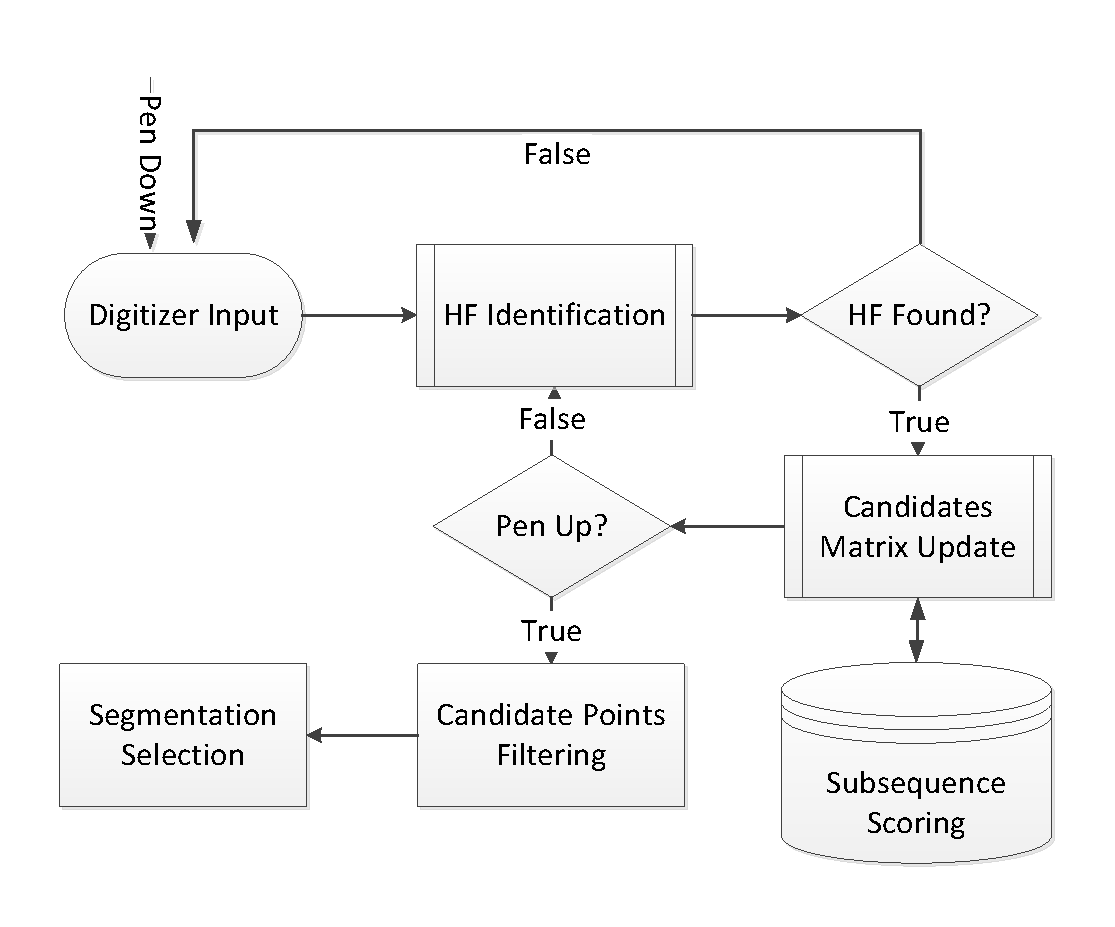
\includegraphics[width=0.8\textwidth]{./figures/system_flow}
\caption{High level visualization of segmentation flow.}
\label{fig:system_flow}
\end{figure}

%%%%%%%%%%%%%%%%%%%%%%%%%%%%%%%%%%%%%%%%%%%%%%%%%%%%%%%
\newpage{}
%%%%%%%%%%%%%%%%%%%%%%%%%%%%%%%%%%%%%%%%%%%%%%%%%%%%%%%

\section{First Stage: POIs Nomination and Sub-strokes Scoring}

\subsection{Horizontal fragment identification} 
In this stage, the system attempts to identify HFs that join pairs of connected letters. 
These handlers are horizontal, directed right to left and located near the baseline (see Figure  \ref{fig:horizontal_fragments}). 
Using a smoothed version of the trajectory helps the process to ignore undesired small horizontal regions that are frequently caused by the digitizer's imperfection.  
A point $p_{i}$ is defined as a "horizontal point" if the slope of the line $\overline{p_{i-1}p_{i}}$ is less than a pre-set value $\delta$, which was empirically tuned to $0.6$. 
The same exact value for this parameter was found independently in \cite{daifallah2009recognition}.

\begin{figure}
\centering
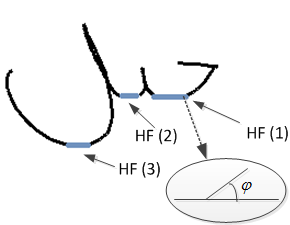
\includegraphics[width=0.3\columnwidth]{./figures/horizontal_fragments}
\caption{Horizontal Fragments (HFs) of the word \RL{jbl} /JABAL/.}
\label{fig:horizontal_fragments}
\end{figure}

HFs are continuously identified using the following process.
The first detected horizontal point is set as an "HF starting point". 
All the subsequent horizontal points are ignored until a non-horizontal point is detected, indicating the end of an HF sequence. 
This point is identified as an "HF ending point" and the medial point of an HF is marked as POI. 
POIs are potential SPs, thus, this process yields an over-segmentation of the stroke. 
While false positive SPs can be easily removed in a latter stage, missed SPs cannot be easily recovered. 
Therefore, in order to minimize the miss-rate, this process is delicate and allows false HFs to be detected.

Once an HF is detected the sub-stroke that spans from the previous POI to the POI of the current HF is checked to make sure they do not reside on the same HF. 
Inn case they do, both HFs are rejoined to a single HF. 
This is done to avoid fractions of the same HF to identified as multiple HFs, 
The merging is done by evaluating the complexity measurement across the two consequent HFs, see Figure \ref{fig:candidate_in_no_horizontal}.

\begin{definition}
\textbf{Complexity measure} is a value that indicates the curvature degree of a given 2-D trajectory $T=\{p_i\}_{i=1}^{n}$. 
Preprocessing steps, which include simplification and re-sampling, are required to ensure invariance under scaling and data imperfections. 
The complexity measure is calculated by summing the parameters $\alpha_{k}$ computed for each inner point $p_k$ in $T$ for $2 \leq k \leq n-1$, i.e., 
\begin{equation}
CM(T)=\sum_{k=2}^{n-1}{\alpha_k}.
\end{equation}
where the parameter $\alpha_{k}$ is defined as $\alpha_{k}=\frac{\pi-\phi_{k}}{\frac{\pi}{6}}$ and $\phi_k=\angle(\overline{p_{k-1}p_{k}},\overline{p_{k}p_{k+1}})$.
\end{definition}

\begin{figure}
\centering
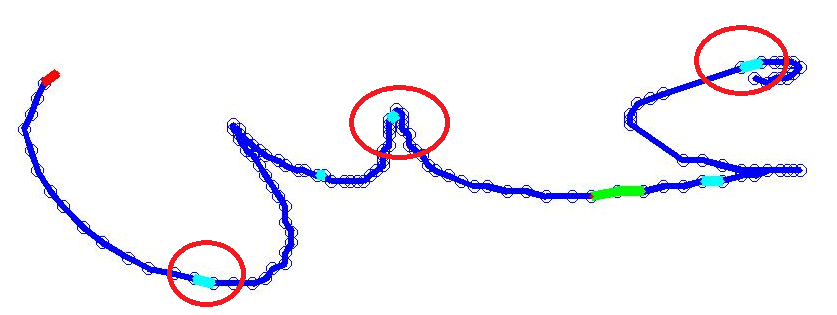
\includegraphics[width=0.3\textwidth]{./figures/candidate_in_no_horizontal}
\caption{The main body of Arabic word \RL{`yn} /AIN/. POIs are colored in cyan. The green areas indicate merge between two subsequent HFs. Three types of false POIs can be seen: 1. A POI at the beginning of a stroke. 2. A POI that is caused by a bad HF. 3. A POI that resides in a letter's valley. }
\label{fig:candidate_in_no_horizontal}
\end{figure}

\subsection{Sub-strokes scoring}
Let $S=\{p_{i}\}_{i=1}^{n}$ be a sequence representing a handwritten stroke in which $L$ POIs were detected. 
Let $KP=\{KP_{i}\}_{i=0}^{L+1}$ (Key points) be the ordered set of the POIs, in addition to the first and the last points of the stroke positioned as the first and the last items in the set.
Formally, we define: 
\begin{equation}
KP_{i} =\begin{cases}    1		, & \mbox{if } i=0 \\
					  POI_{i}	, & \mbox{if } 1\leq i \leq L \\
					       n    , & \mbox{if } i=L+1 
			\end{cases}				
\end{equation}
A sub-stroke $S_{i}^{j}$ is a sub-sequence of the stroke $S$ that starts at $KP_{i}$ and ends at $KP_{j}$, formally:
\begin{equation}
S_{i}^{j}=\{p_{k}\}_{k=KP_{i}}^{KP_{j}}; i<j
\end{equation}

We generate an upper triangular \emph{scoring matrix} $D\in\mathbb{R}^{(L+1)\times (L+1)}$ where each cell $D_{i,j}$ represents the sub-stroke $S_i^j$. 
It contains the classification information and scoring, for the sub-strokes $S_i^j$, returned by the characters classification system described in Chapter \ref{chap:characters_classification}. 
The matrix $D$ is generated dynamically; adding a row and a column for each new detected POI. 
Imposing a locality constraint which narrows the band of the $D$ matrix above the main diagonal improved the efficiency of the process and the segmentation accuracy. 
Given a band width $B$ we fix $D_{i,j}=\infty$ if  $j \leq i$ or $j-i>B$.
We argue that sub-strokes representing a letter will achieve, in most cases, better scoring, i.e., lower $D_{i,j}$ value than other sub-strokes.

\begin{figure}
\centering
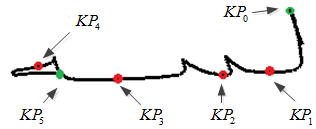
\includegraphics[width=0.4\textwidth]{./figures/candidate_points}
\caption{KPs of the word \RL{lbyh} /Lbyh/. POIs are coloured in red. The first and last KPs are coloured in green. }
\label{fig:candidate_points}
\end{figure}

Using the relative location of the sub-stroke in the stroke we restrict the classification process to search for similar samples feasible position databases.
As can be seen in Table \ref{table:subsequences_types}, we differentiate between four types of sub-sequences.
For each type, we indicate the set of databases that need to be examined, i.e., the possible letter positions the sub-stroke may represent. 
In Table \ref{table:subsequences_types}, $S$ denotes a stroke containing $L$ POIs where $m>0$ and $k<L+1$.

\begin{table}
\centering
\renewcommand{\arraystretch}{1.3}
\caption{A mapping between the subsequence types and the possible letter positions.}
\begin{tabular}{| c | c | c |}
\hline
  \textbf{Subsequence Symbol}     & \textbf{Subsequence Location}    & \textbf{Possible Letter Position}     \\
\hline
  $\alpha$ & $S_0^{k}$      & $Ini$ or $Mid$      \\
\hline
  $\beta$  & $S_{m}^{k}$    & $Mid$               \\
\hline
  $\chi$   & $S_{m}^{L+1}$ & $Mid$ or $Fin$       \\
\hline
  $\delta$ & $S_0^{L+1}$    & All                 \\
\hline
\end{tabular}
\label{table:subsequences_types}
\end{table}

The relation between the cells in the matrix $D$ and the sub-stroke type is given in matrix $D_p$  (Equation \ref{eq:positions_matrix}). 
The type of the sub-stroke can be determined while the stroke is being scribed.
The last column and row are added on the "pen up" event.

\begin{equation}
D_{p}=
\left( 
\begin{array}{ccccccc}
\infty 	& \alpha & \alpha & \alpha  & \cdots & \alpha & \delta      \\
\infty  & \infty  & \beta   & \beta   & \cdots  & \beta  & \chi     \\
\infty  & \infty  & \infty   & \beta   & \cdots  & \beta  & \chi    \\
\vdots & \vdots & \vdots  & \vdots & \ddots  & \vdots & \vdots      \\
\infty  & \infty  & \infty   & \infty   & \cdots  & \beta  & \chi   \\
\infty  & \infty  & \infty   & \infty   & \cdots  & \infty  & \chi  \\
\infty  & \infty  & \infty   & \infty   & \cdots  & \infty  & \infty \end{array} \right)
\label{eq:positions_matrix}
\end{equation}\\

For a given input (sequence and position), the recognition system returns the $K$ nearest neighbors with different labeling, where the labeling is defined as the tuple (letter, position). In our implementation, we set $K=3$.

\begin{figure}
\centering
\begin{tabular}{| c |c | c | c| c | c | c |}
\hline
     & $0$ & $1$ & $2$ & $3$ & $4$ & $5$\\
\hline
$0$
   & N/A
   & \subfloat{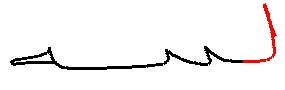
\includegraphics[width=1.8cm]{./figures/substrokes/L}}
   & \subfloat{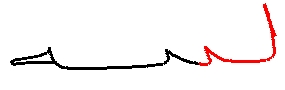
\includegraphics[width=1.8cm]{./figures/substrokes/LB1}}
   & \subfloat{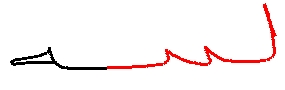
\includegraphics[width=1.8cm]{./figures/substrokes/LB1B2}}
   & N/A & N/A \\
\hline
$1$
   & N/A & N/A
   & \subfloat{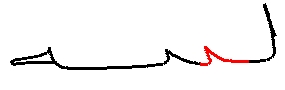
\includegraphics[width=1.8cm]{./figures/substrokes/B1}}
   & \subfloat{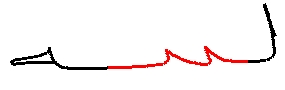
\includegraphics[width=1.8cm]{./figures/substrokes/B1B2}}
   & \subfloat{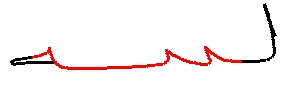
\includegraphics[width=1.8cm]{./figures/substrokes/B1B2H1}}
   & N/A \\
\hline
$2$
   & N/A  & N/A & N/A
   & \subfloat{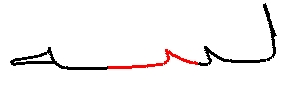
\includegraphics[width=1.8cm]{./figures/substrokes/B2}}
   & \subfloat{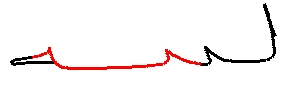
\includegraphics[width=1.8cm]{./figures/substrokes/B2H1}}
   & \subfloat{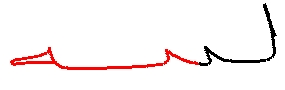
\includegraphics[width=1.8cm]{./figures/substrokes/B2H}} \\
\hline
$3$
   & N/A & N/A & N/A & N/A
   & \subfloat{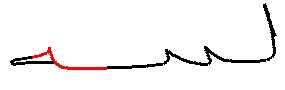
\includegraphics[width=1.8cm]{./figures/substrokes/H1}}
   & \subfloat{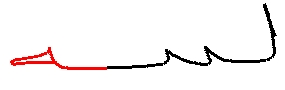
\includegraphics[width=1.8cm]{./figures/substrokes/H}} \\
\hline
$4$
   & N/A & N/A & N/A & N/A & N/A
   & \subfloat{
\includegraphics[width=1.8cm]{./figures/substrokes/H2}}\\
\hline
$5$
   & N/A & N/A & N/A & N/A & N/A & N/A \\
\hline
\end{tabular}
\caption{A tabular representation of the $D$ matrix that corresponds the KPs showed in Figure \ref{fig:candidate_points}. Each cell visually demonstrates the matching sub-stroke colored in red.}
\label{table:substrokes_demo} 
\end{figure}

%%%%%%%%%%%%%%%%%%%%%%%%%%%%%%%%%%%%%%%%%%%%%%%%%%%%%%%
\newpage{}
%%%%%%%%%%%%%%%%%%%%%%%%%%%%%%%%%%%%%%%%%%%%%%%%%%%%%%%

\section{Second Stage: POI Filtering and Scoring Correction}
In this stage we re-score subsequences and eliminate redundant POIs based on the following rules:

\begin{compactitem}
	\item SPs should lie close to the baseline. 
	\item SPs do not reside in loops.
	\item The sub-stroke length should be proportional to the length of the containing stroke.
\end{compactitem}

The system determines the baseline by calculating the vertical projection histogram of the re-sampled and normalized version of the stroke. 
The height of the stroke (y-axis) is partitioned into ten equi-length intervals. 
A POI is filtered out if it does not satisfy the following condition:
\begin{equation}
|POI_y-I_{max}| \leq 2 max{({|I|},0.15)} 
\end{equation}
where $POI_y$ represents the $y$-coordinate of the POI; $|I|$ is the length of an interval; and $I_{max}$ denotes the center of the most inhabited interval. 
In order to reliably determine the baseline, the baseline detection algorithm is activated only after the fourth POI is detected.
This process has proven to be very effective in eliminating challenging false POIs that reside in valleys of frequently used final Arabic letters, such as \RL{-q}, \RL{-s} and \RL{-n}. 
An example of such a POI can be seen in the letter \RL{-n} in Figure \ref{fig:candidate_in_no_horizontal}. 
Determining the baseline using the vertical projection histogram is a commonly used technique \cite{burrow2004arabic, bagdanov1997projection}.


The baseline is needed only to verify that the POIs are in a reasonable distance from it, therefore, imprecise valuation of the position or the direction of the baseline is tolerable.

\begin{figure}[b]
\centering

\includegraphics[width=0.8\textwidth]{./figures/baseline}
\caption{The position of the baseline corresponds to the largest peak of the vertical projection histogram \cite{burrow2004arabic}.}
\label{fig:candidate_in_no_horizontal}
\end{figure}

In order to identify SPs that resides inside a loop we have employed a Matlab package that includes an implementation for poly-line intersection algorithm \cite{legland2014geom2d}.

The third rule is used to penalize unreasonably low scoring given to small sub-strokes, which are unlikely to represent a letter. 
This is done by calculating the ratio of the sub-stroke length proportional to the entire stroke length.
For instance, it is common to add a small, hook-like, extension to the suffix of the letter \RL{d}. 
This extension may look very similar to the letter \RL{-a} during the stroke scribing; and thus under-scored, i.e. is given a very good similarity measure by the recognition system, and eventually result in over-segmenting the letter \RL{d}. 

In some cases, POIs are incorrectly nominated on non-horizontal areas. This is caused due to noises in the data and the fact that the nomination is done while the word is being scribed. Our filtering algorithm should be corrected, in a future work, to handle this case.

%%%%%%%%%%%%%%%%%%%%%%%%%%%%%%%%%%%%%%%%%%%%%%%%%%%%%%%
\newpage{}
%%%%%%%%%%%%%%%%%%%%%%%%%%%%%%%%%%%%%%%%%%%%%%%%%%%%%%%

\section{Third Stage: Segmentation Selection}
The goal of this phase is to select the set of SPs among the POIs. 
This set will be referred to as the \emph{final segmentation points} (FSP). 
It is performed by finding the \emph{segmentation path} in $D$ with the best scoring possible. 
A segmentation path $\pi$ is an ordered subset of the KPs and must contain $KP_{0}$ and $KP_{L+1}$ as the first and the last points in the path.
$\Pi$ denotes the scoring of the segmentation path $\pi$. 
It is defined as the summation of the sub-sequences scoring in the segmentation path divided by the path length; this is done in order to prevent giving superiority to under-segmentations.

One can model the scoring matrix $D$ as a directed, edge-weighted graph $G=(V,E)$, for which a path from vertex $KP_0$ to vertex $KP_{L+1}$ defines a possible segmentation. 
It can be experimentally validated that finding the shortest path in $G$ (from $KP_0$ to $KP_{L+1}$) does not necessarily obtain the optimal segmentation, and in some cases, produces under-segmentation of the stroke. 
It is because the shortest path is a global property, which may prefer a highly weighted shortcut path over a path that consists of several low weighted fragments; in cases where the accumulative weight of the fragmented path is larger than the shortcut path.
However, greedily selecting the outgoing edge with the minimal weight will mostly return a better segmentation.

Several \emph{segmentation selection algorithms} (SSAs) for finding the best segmentation path are proposed in this work.
Here we describe two algorithms that were given the names \emph{Forwards Segmentation Selection} (FSS) and \emph{Backwards Segmentation Selection} (BSS) which operate quite similarly. 
A pseudo-code of FSS algorithm can be seen in Algorithm \ref{alg:fss}. 
FSS starts with the first point, $KP_0$, advancing toward the end of the stroke. 
In Each step, it tries to find the next best KP by selecting the adjacent subsequence $S_i^j$ with the best scoring (as can be seen in line 5). 
BSS operates similarly but starts from the last point and advances toward the beginning of the stroke. 
The main drawback of these two algorithms is that FSS tends to under-segment the suffix of the stroke and BSS tends to under-segment the stroke's prefix.

\begin{algorithm}
$\pi = \{0\} $\;
$i=0$\;
$sum=0$\;
\While{$i<L+1$}
{
	$j = \mathop {\arg \min }\limits_k \left( {D\left( {i,k} \right)} \right)$\;
	$\pi = \pi \cup \left\{ j \right\}$\;
	$sum = sum + D\left( {i,j} \right)$\;
	$i=j$\;
}
\caption{Forwards Segmentation Selection (FSS) algorithm.}
\label{alg:fss}
\end{algorithm}

In an attempt to overcome the aforementioned drawbacks, a third SSA is proposed, and given the name \emph{Backwards-Forwards Segmentation Selection} (BFSS). 
As can be seen in Algorithm \ref{alg:bfss}, it combines both FSS and BSS. 
BFSS operates from the sides of the stroke toward the center. In every iteration, it selects two candidate points to include to the segmentation path.

\begin{algorithm}
$\pi = \{0,L+1\}$\;
$kp_{a}=0$\;
$kp_{b}=L+1$\;
\While{$kp_{a}<kp_{b}$}
{
	$kp_{a,next} = \mathop {\arg \min}\limits_k (D(kp_a,k))$\;
	$\pi = \pi \cup \{kp_{a,next}\}$\;
	$kp_{a}=kp_{a,next}$\;
	
	$kp_{b,next} = \mathop {\arg \min}\limits_k (D(k,kp_{b,next}))$\;
	$\pi = \pi \cup \{kp_{b,next}\}$\;	
	$kp_{b}=kp_{b,next}$\;
}
\caption{Backwards-Forwards Segmentation Selection (BFSS) algorithm.}
\label{alg:bfss}
\end{algorithm}
  
The last algorithm was given the name \emph{Greedy Segmentation Selection} (GSS) and is described in Algorithm \ref{alg:gss}.
GSS operates differently. In every iteration, the cell with the lowest (best) scoring is selected. 
Once a cell $D_{i,j}$ is selected, since it represents the sub-stroke $S_{i}^{j}$, both $KP_{i}$ and $KP_{j}$ are added to the FSP, and every cell corresponding to a subpart of the sub-stroke $S_{i}^{j}$ is removed by setting its corresponding scoring value in the matrix $D$ to $\infty$; in order to avoid those sub-strokes to be selected in a later iteration. In Algorithm \ref{alg:gss}, the notation $[\infty]^{(L+1)\times (L+1)}$ indicates a matrix that all it's cells are set to $\infty$.
 
\begin{algorithm}
$\pi = \{0,L+1\}$\;
\While{$D \neq [\infty]^{(L+1)\times (L+1)}$}
{
	${s,e} = \mathop {\arg \min}(D)$\;
	$\pi = \pi \cup \{s,e\}$\;
	$sum = sum + D(s,e)$\;
	$UpdateMatrix(D,s,e)$\;
}

\caption{Greedy Segmentation Selection (GSS) algorithm.}
\label{alg:gss}
\end{algorithm}

Performance evaluation of the mentioned SSA is provided in \ref{subsec:ssa_performance}.


%%%%%%%%%%%%%%%%%%%%%%%%%%%%%%%%%%%%%%%%%%%%%%%%%%%%%%%
\newpage{}
%%%%%%%%%%%%%%%%%%%%%%%%%%%%%%%%%%%%%%%%%%%%%%%%%%%%%%%

\section{Experimental Results}
\label{sec:segmentation_results}
Comparing the performance of the real-time segmentation approach described in this work to results obtained by related researches is difficult due to the different experimental settings, databases and methodology; not to mention the different measures used to present the results. 
The usage of the ADAB database, instead of a self-collected database, standardize and reinforces our results. 
In Table \ref{table:general_stats}, we provide basic statistics of our sample set. 
Table \ref{table:segmentation_results} summarizes the system's performance.

\begin{table}[b]
\renewcommand{\arraystretch}{1.2}
\centering
\caption{Segmentation sample set general statistics.}
\begin{tabular}{ | c | c | }
  \hline
  Number of test samples (city name) & 319 \\
  \hline
  Number of WPs & 1148 \\
  \hline
  Number of Strokes & 1237 \\
  \hline
\end{tabular}
\label{table:general_stats} 
\end{table}

\begin{table}[b]
\renewcommand{\arraystretch}{1.2}
\centering
\caption{Segmentation results.}
\begin{tabular}{ | c | c | }
  \hline
  Strokes segmentation rate &  83\% \\ 
  \hline
  Strokes recognition rate &  78\% \\ 
 \hline
  Total number of true SPs & 1081 \\
  \hline
  Valid SPs (True Positive) & 85.3\% \\
    \hline
  Missing SPs (False Negative) & 14.7\% \\
  \hline
  Invalid SPs (False Positive) & 119 (11\%) \\
  \hline                                    
  SPs Precision & 88.6\% \\ 
 \hline
  SPs Recall &  85.3\% \\ 
 \hline
\end{tabular}
\label{table:segmentation_results} 
\end{table}

\subsection{Validation}
\label{subsec:validation}
Related researches usually use a human expert to validate the accuracy of the SPs. However, in this work, we applied an automatic validation process using the ground truth information provided by the database. We discriminate between three types of final SPs. A final SP is classified as true positive if the complexity measure between the identified point and a true SP is less than a preset threshold; otherwise, it is classified as false positive. A false negative (miss), is the case when the system failed to identify a true SP. The different types of SPs can be seen in Figure \ref{fig:sp_types}.
The validation process was tested on several sets and found to be highly reliable.

\begin{figure}[b]
\centering
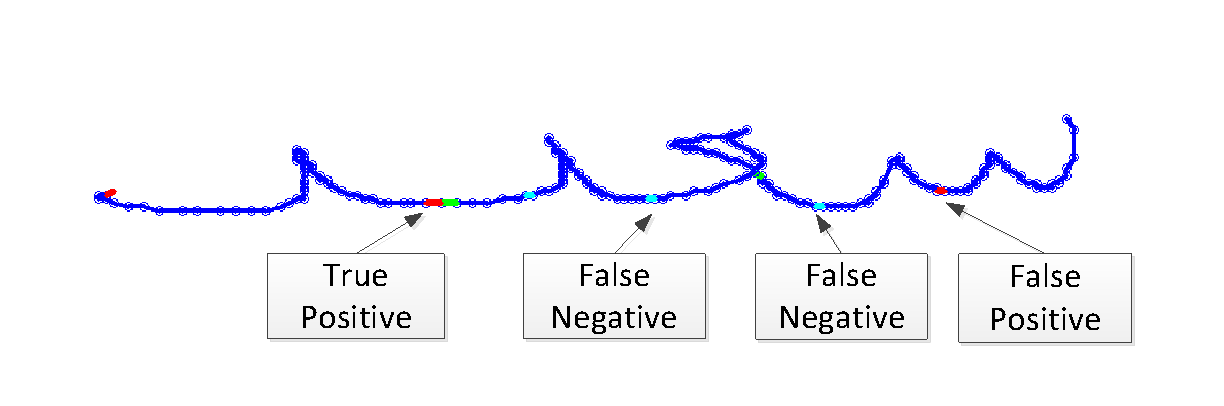
\includegraphics[width=0.6\textwidth]{./figures/sp_types}
\caption{SPs types.}
\label{fig:sp_types}
\end{figure}

\subsection{Analysis}
In this section we discuss common cases of incorrect segmentation.\\
\subsubsection{Over-segmentation}
\begin{itemize}
\item Several Arabic letters contain a horizontal region in their initial form which does not accommodate a SP, see Figure \ref{fig:candidate_in_no_horizontal}. 
We overcame this problem by adding the following rule: a POI is nominated only if the sub-stroke that spans from the beginning of the stroke to the POI has a high complexity measure.
\item Over-segmentation can also be caused by typing a letter in unusual form where it is spanned over several strokes. 
It happens mostly in the letter \RL{-m-}, \RL{-m} and in rare cases in the letter \RL{-.h-}. This issue will be addressed in a future work.
\end{itemize}

\begin{figure}
\centering
        \subfloat[]{
            \label{fig:letters_same_body_1}
            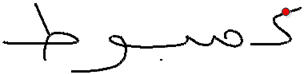
\includegraphics[width=0.3\textwidth]{./figures/oversegmentation_begin_1}
        }
        \subfloat[]{
           \label{fig:letters_same_body_2}
           
\includegraphics[width=0.15\textwidth]{./figures/oversegmentation_begin_2}
        }        
    \caption{Samples of redundant Candidate point at the beginning of the stroke.}
   \label{fig:oversegmentation_begin}
\end{figure}

Without the additional strokes, there is no way to differentiate between the main body of the letter \RL{-s-} /s/ and the main body of two consecutive \RL{-b-} /b/ (or other identical main body letters as seen in figure \ref{fig:same_body_letters}). 


\begin{figure}
\centering
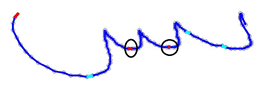
\includegraphics[width=5cm]{./figures/oversegmentation_s}
\caption{Over-segmentation in the letter \RL{-s-}. appearance to a combination of two consecutive \RL{-b-} letters and only can be identified from the context and using the additional strokes.}
\label{fig:oversegmentation_s}
\end{figure}

\subsubsection{Under-segmentation}
\begin{itemize}
\item Letter pairs that are not separated by HFs cause the system to miss POIs. This was partially solved by extending the notion of a letter to include such pairs. For example the pair \RL{lm} and \RL{l.h}.
\item In some cases, HFs were identified correctly but the corresponding POI were not selected in the third stage. This may result from nomination of a candidate point on correct horizontal segment but in a late fraction of the segmentation fragment which result in a low scoring and thus not being selected by the SSA. This issue usually occurs in the letter \RL{w} in its final position (Figure \ref{fig:undersegmentation_w}).
\end{itemize}

\begin{figure}
\centering
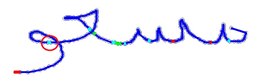
\includegraphics[width=5cm]{./figures/undersegmentation_w}
\caption{An example of a late candidate point in the letter \RL{w}.}
\label{fig:undersegmentation_w}
\end{figure}

We have noticed that the absolute majority of the false negative (missed) SPs were actually identified as POIs in the first stage, but were not selected by the SSA.
In addition, differentiating between the main body of the letter \RL{-s-} and the main body of two consecutive \RL{-b-} letters is possible only when considering the additional strokes, thus both cases were considered to be correct.

\subsection{Segmentation Selection Algorithms Performance}
\label{subsec:ssa_performance}
It is apparent from the data in Table \ref{table:ss_algorithms_results}, that the SSA has a crucial effect on the system's performance. 
We tested several combinations of two SSAs in which the FSP is found by executing both SSAs independently and selecting the segmentation path with the smallest scoring. In Table \ref{table:ss_algorithms_results}, a combination of two algorithms is denoted by $\oplus$.

\begin{table}
\centering
\caption{Comparing the different SSAs performance.}
\begin{tabular}{ | c | c | c | c | c |}
\hline
\textbf{SSA} & \textbf{WP segmentation} & \textbf{WP recognition} & \textbf{SP precision} & \textbf{SP recall}\\
             & \textbf{rate}            & \textbf{rate}           &                       &\\  
\hline                 
  FSS & 76\% & 70\% & 85\% & 78\% \\ 
  \hline
  BSS & 79\% &  73\% & 84\%& 81\% \\
  \hline
  BFSS & 78\% & 72\% & 84\% & 80\%\\ 
  \hline
  GSS & 80\% & 74\% & 81\% & \bf{94}\% \\  
  \hline
  FSS$\oplus$BSS & \bf{82}\% & \bf{76}\% & \bf{89}\% & 82\%\\  
  \hline
  GSS$\oplus$BFSS & 81\% & 75\% & 83\% & 90\% \\
  \hline
\end{tabular}
\label{table:ss_algorithms_results} 
\end{table}

\subsection{Sample set size and distribution}
The letters is our training set are extracted from a database with a limited words diversity, thus, the distribution of the samples between the different classes is imbalanced. 
On one hand, it can be regarded as an advantage; since, the training set distribution reflects the a-priory probability of a letter appearance in the test set. 
On the other hand, a highly imbalanced training set is known to negatively affect many classification algorithms.
In the following experiment, we measure the effect of a large and imbalanced training set on the WP segmentation and recognition rates. 
It is done by gradually increasing the maximal allowed number of samples per class (letter and position).
 
The graph in Figure \ref{fig:num_letter_impact} shows convergence of the system's performance when the maximal number of samples is larger than 200 per class. 
Nevertheless, a miniature degradation is apparent, which is caused, probably, due to the increasing imbalance in the distribution of the training set.
In addition, it is evident that the recognition rate is more sensitive to small training set than the segmentation rate.

\begin{figure}
\centering
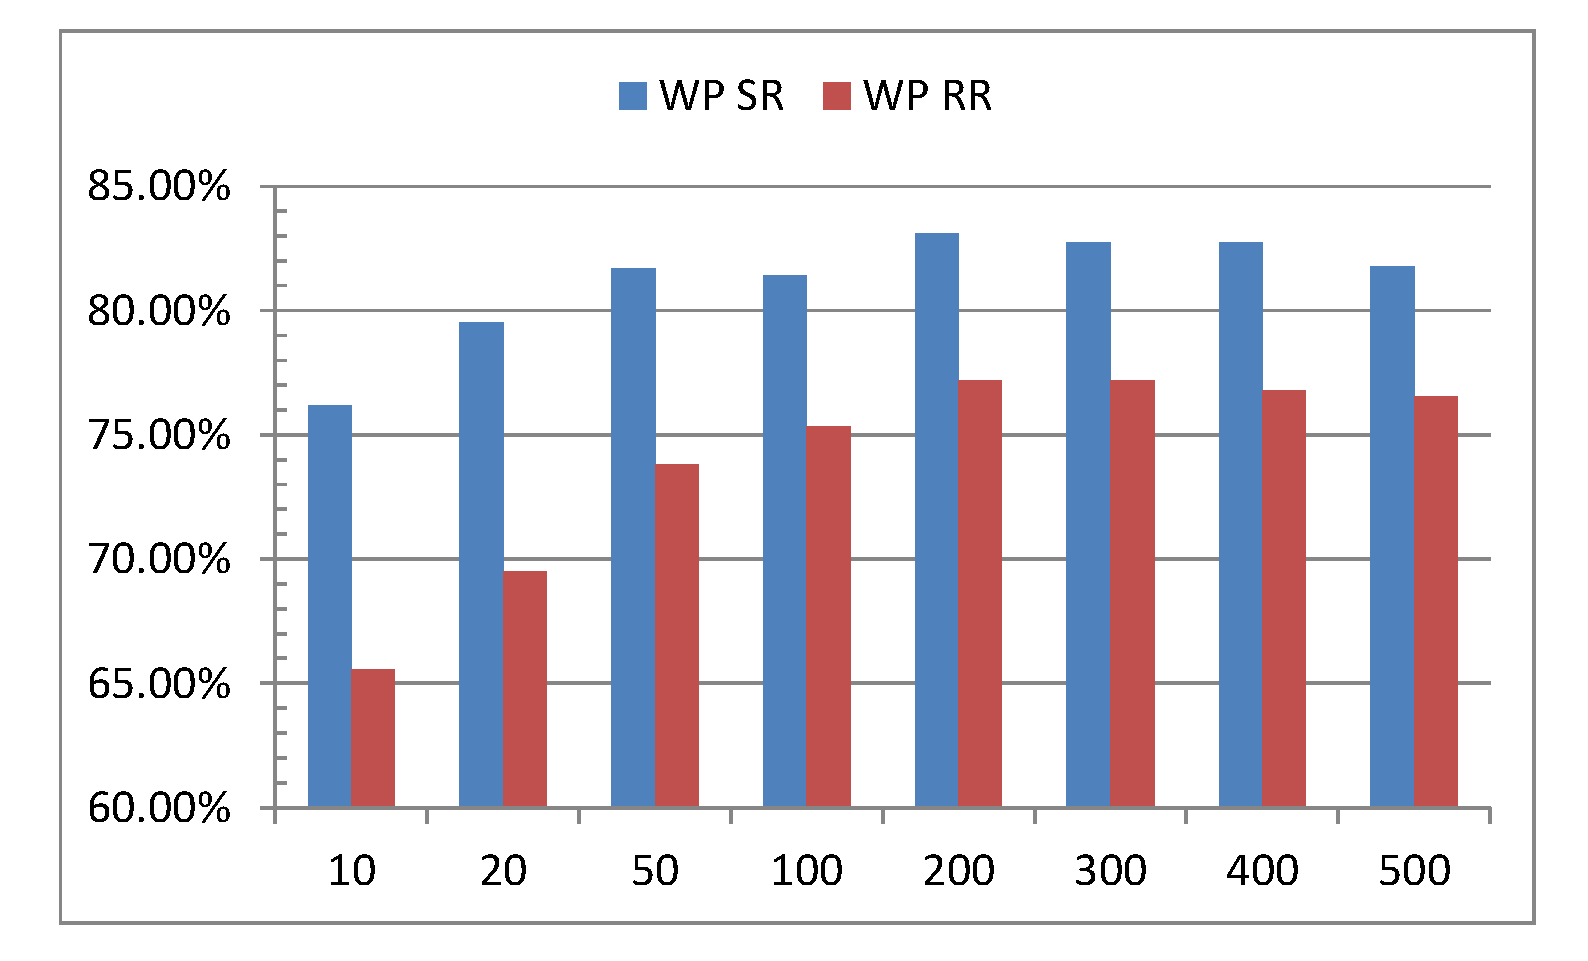
\includegraphics[width=0.7\textwidth]{./figures/num_letter_impact}
\caption{The impact of increasing the maximal number of samples per class on the segmentation and recognition rates.}
\label{fig:num_letter_impact}
\end{figure}

%%%%%%%%%%%%%%%%%%%%%%%%%%%%%%%%%%%%%%%%%%%%%%%%%%%%%%%
\newpage{}
%%%%%%%%%%%%%%%%%%%%%%%%%%%%%%%%%%%%%%%%%%%%%%%%%%%%%%%

\section{Holistic WPs Recognition Using Characters Classification Information}
\label{sec:wps_recognition}
As mentioned earlier, the segmentation and classification information obtained by a real-time segmentation system, can be used to significantly reduce the potential dictionary size and accelerate a later holistic recognition process as follows:
\begin{compactitem}
\item In an open-vocabulary environment, the classification information can be employed to dynamically build a class of different shapes for all possible WPs.
\item In a closed-vocabulary environment, a holistic recognition approach can be limited to consider valid combination that appear in the vocabulary. 
\end{compactitem}

In this section we evaluate the recognition accuracy that can be obtained in the an open-vocabulary environment.
Following the real-time segmentation process, the $10$ top scored candidates of each character are recorded. 
These shapes are used to generate a complete list of all possible shape concatenation of the retrieved candidates. 
The obtained candidates represent different shapes of the same letter producing multiple shapes of the same WP. 
The cardinality of the generated list is $10^p$ where $p$ is the predicted number of characters in the WP using the segmentation process. 
The large size of the generated list, which may exceed $10,000$ shapes, requires a similar process of embedding and dimensionality reduction, as described above, to generate a short list of candidates. 
The short list of candidates in the next step is matched against the queried WP using the original expensive and more accurate matching process. 
Using the proposed approach, the $10$ top WPs results yield a $98.1\%$ recognition rate. 
The recognition rate of the first top candidate dropped down to $90.8\%$. 
Using a voting process within the top five results gave a $94.7\%$ recognition rate. 

Analysing the failures of the misclassified samples shows that most recognition errors occur as a result of misclassifying a single character. 
In most cases the misclassified character is confused with a character having a very similar shape, which can be corrected using information retrieved by the associated additional stroke, such as the case of the letter \RL{-l} /l/ and the letter \RL{-n} /n/ in their handwritten form.


%\bibliographystyle{plainnat}
%\bibliography{references}
%
%\end{document}

%%% LyX 2.0.5.1 created this file.  For more info, see http://www.lyx.org/.
%%% Do not edit unless you really know what you are doing.
%\documentclass[twoside,english]{report}
%\usepackage[T1]{fontenc}
%\usepackage[latin9]{inputenc}
%\setcounter{secnumdepth}{3}
%\setcounter{tocdepth}{3}
%\usepackage[active]{srcltx}
%\usepackage{verbatim}
%\usepackage{graphicx}
%\usepackage{setspace}
%\usepackage[numbers]{natbib}
%\doublespacing
%
%\makeatletter
%
%%%%%%%%%%%%%%%%%%%%%%%%%%%%%%% LyX specific LaTeX commands.
%\providecommand{\LyX}{L\kern-.1667em\lower.25em\hbox{Y}\kern-.125emX\@}
%%% Because html converters don't know tabularnewline
%\providecommand{\tabularnewline}{\\}
%
%\makeatother
%
%\usepackage{babel}
%\begin{document}

\chapter{Summary, Conclusions and Future Work}
\label{cahp:conclusions}

In this thesis we have proposed and implemented a system to recognize Arabic online handwriting script. Our approach successfully tackled many inherent difficulties in recognizing Arabic script such as segmentation of word parts, non-horizontal writing style, position-depended letter shaping and large word-part dictionary which has been overcome upon by combining both the analytic and the heuristic approach. We compared the Shape context to the MAD descriptor and showed that the MAD descriptor attained higher recognition rate. A novel online segmentation technique was introduced and used in the analytic phase. The Linear EMD embedding technique was used as a metric in the classification algorithms and showed promising results in measuring letters and word parts grasped dissimilarity. A contemporary composition of PCA and LDA, based on the method previously proposed in [18], was applied in the system and achieved qualitative dimensionality reduction. This approach can be used to overcome the "curse of dimensionality" in other fields of pattern recognition. We have integrated fast data retrieval methods to boost the performance of the system. The system demonstrated superior high recognition precision and low response time.
The system has several limitation and assumptions that are not always true in the field of Arabic handwriting; first, the system does not regard additional strokes, which can be used to improve the classification results; second, it assumes that letters cannot be written in more than one stroke which is a very reasonable assumption however not always true. Our future work will focus on waiving these limitations. Also we plan to test this approach on other cursive handwriting styles of languages other than Arabic. 


\section{Future Directions}
In future direction we would like to rid of all the limitation mentioned in the limitation section.
We have several directions we would like to develop. In this work we did not consider the additional strokes written and we tried to recognize only the main body of the written text. In future work we would like to be able to recognize the whole letter and use the additional strokes to be able to identify the exact letter written.
The following enhancement will be introduced to the process in a future work: 1. Since the embedding is done to the L1 space, we will try to use L1 dimensionality reduction techniques such as L1-PCA and L1-LDA. 2. We can add Metric Learning techniques such as LMNN to improve our recognition rate. 3. In this work all shapes that belong to the same letter are ascribed to the same cluster although it might look totally different, in our future work we will create more that cluster to the same letter to represent the main shapes that are common to describe a letter.[??] 4. The use of more advanced clustering techniques to reduce the number of samples in the training set and which will accelerate the classification process.
Also, we are planning to develop a word completion algorithm based on our ongoing recognition technique. The word completion feature is actually  will suggest the user to automatically complete the word the user has intended to write, based on the first letters written by him. 
We also plan to connect a word parts or words database to the recognition system, which will certainly improve the recognition rate dramatically. However it will limit the recognized word/word parts to the dictionary.


\section{Summary and Future Work}
In this paper, we proposed a ongoing approach for segmenting open-dictionary, Arabic handwritten script.
The segmentation is performed in the strokes level. 
Morphological features are employed to nominate potential SPs. 
The sub-strokes induced by the SPs are classified using a $k$-NN letters classifier, and the classification information is saved in a scoring matrix.
The final segmentation points are then selected by finding the best-scored segmentation path in the scoring matrix. 
This is done using several proposed algorithms. 
The system has demonstrated promising results.

In future work, we will expand the process by adding a later holistic WP recognizer that exploits the proposed segmentation and the scoring information to inspect a limited number of potential WPs.\\

\begin{itemize}
\item The use of the temporal information of the written for both classification and segmentation. Since on-line handwritten script give us this information we better use it to enhance our system. 
\item use more sophisticated segmentation techniques and rules. i.e. instead of using the static rules to detect segmentation points.   
\end{itemize}



%\end{document}


\bibliographystyle{plainnat}
\bibliography{references}

\appendix
\documentclass[12pt,english]{report}
\usepackage{mathptmx}
\renewcommand{\familydefault}{\rmdefault}
\usepackage[T1]{fontenc}
\usepackage[latin9]{inputenc}
\usepackage[a4paper]{geometry}
\setcounter{secnumdepth}{2} % Changed from 3 to 2. 0-chapter 1-section 2-subsection 
\setcounter{tocdepth}{2} % Changed from 3 to 2. 0-chapter 1-section 2-subsection 
\setlength{\parskip}{\medskipamount}
\setlength{\parindent}{0pt}
\usepackage{verbatim}
\usepackage{pdfpages}
\usepackage{graphicx}
\usepackage{subfig} %% This package has to be here
\usepackage{setspace}
\usepackage{arabtex}
\usepackage[numbers]{natbib}
\usepackage{nomencl}
\usepackage{amsthm}
\usepackage{amsfonts}
\begin{document}

\chapter{Wavelets and the wavelet transform}

The topic of wavelet analysis is relatively a new concept. To fully comprehend the subject one usually needs to investment a large amount of time in studying the subject. In addition, it requires a high level of mathematical background, which is usually not covered in a basic calculus courses.
The Wavelet transform, like the Fourier transform, is used in many fields of mathematics, physics and engineering. Quite a few articles and books were written on the subject, therefore, here we attempt to provide a short and intuitive introduction to the topic and let the interested reader to learn more about the subject in the literature. The reader is referred to \cite{meyer1992wavelets} for an exhaustive discussion on the wavelet transform.\\ 

Recall that the Fourier Transform gives the frequency information of a signal, namely, it provide us information about the frequencies that can be found in the signal. However, it does not indicate on what time exactly these frequency components exist. In cases where the signal is stationary, this information is unneeded. FT can also be used for non-stationary signals, if we are only interested in what frequency components exist in the signal, but are not required to know where in time these frequencies occur. Nevertheless, if we want to know what frequency component occur at what time (interval), then Fourier transform is not the best transform to use. Wavelet transform is provide us with the time-frequency representation of the signal and thus give us information about the both the time and frequencies.\\

Wavelets may be seen as small waves $\psi(t)$, which oscillate few times, but unlike the harmonic waves ($sin(nx)$ and $cos(nx)$ on $(-\pi,\pi]$) must die out to zero as $t \rightarrow \pm\infty$. The most applicable wavelets are those that die out after a few oscillations on a finite interval $[a,b)$. \\

The wavelet transform aims to convert a signal into a series of wavelets and by doing so to provide a way for analyzing waveforms bounded in both frequency and duration. This is done to provide information that is not obvious in the original time domain function and also to allow signals to be stored efficiently and to be able to better approximate real-world signals. \\

\begin{equation}
\Psi^{\psi}_{x}(\tau, s)=\frac{1}{\sqrt{|s|}}\int{x(t)\psi^*(\frac{t-\tau}{s})dt}
\label{eq:wavelet_decomposition}
\end{equation}
As seen in the above Equation \ref{eq:wavelet_decomposition}, the transformed signal is a two variables function, $\tau$ and $s$ , the translation and scale parameters respectively. $\psi(t)$ is called the mother wavelet.\\

The scale parameter $s$ can be though of as exactly the scaling in maps. High scales correspond to a non-detailed high level view (of the signal), and low scales correspond to a detailed low level view. Similarly, in terms of frequency, low frequencies (high scales) correspond to a global information of a signal (that usually spans the entire signal), whereas high frequencies (low scales) correspond to a detailed information of a hidden pattern in the signal (that usually lasts a relatively short time).\\

The idea of the wavelet transform is analyzing a signal function $f(x)$ by creating a mathematical structure that vary in scale. i.e., construct a function, shift it by some amount, change its scale. Repeat the procedure to obtain a new approximation. This is usually refereed to as a \emph{multiresolution analysis}. In order to analyze a non-stationary signal, we need to determine its behavior at any individual event. Multi-resolution analysis provides one means to do this. A multi-resolution analysis decomposes a signal into a smoothed version of the original signal and a set of detail information at different scales. Once we have decomposed a signal this way, we may analyze the behavior of the detail information across the different scales.\\

The fundamental idea of wavelet transforms is that the transformation should allow only changes in time extension, but not in the shape of the wavelet. 
A function $f$ in $\mathbb{R}$ can be expressed in terms of wavelet series as follows:
\begin{equation}
f(x)=\sum\limits_{k}{f_k \phi(x-k)}+\sum\limits_{k}{f_{j,k}\psi_{j,k}(x)}
\end{equation}

where $\phi$ is the scaling function and $\psi$ is the wavelet. $k$ runs through all integer and represents shifts.\\


\end{document}


\newpage{}

\includepdf[pages=-]{hebrew_part}
\end{document}
